\documentclass[12pt]{book}
\usepackage[utf8]{inputenc}
\usepackage[french, english]{babel}
\usepackage[T1]{fontenc}
\usepackage{lipsum}

\usepackage{amsfonts}
\usepackage{amsmath}
\usepackage{amssymb}
\usepackage[mathscr]{euscript}
\usepackage{stmaryrd}
\usepackage[normalem]{ulem}
\usepackage{tikz,tikz-3dplot}
\usepackage{tikz-cd}
\usepackage{pgfplots}
\usepackage{graphicx}
\usepackage{color}
\usepackage{enumitem}
\usetikzlibrary{matrix,chains,positioning,decorations.pathreplacing,arrows}
% \usetikzlibrary{external}
% \tikzexternalize[prefix=tikzext/]
% \tikzset{external/mode=graphics if exists}
\usepackage{framed}
\usepackage{arydshln}
\usepackage{multirow}
\usepackage{mathtools}
%\usepackage{float}
%\usepackage{yhmath}
\DeclareSymbolFont{yhlargesymbols}{OMX}{yhex}{m}{n}
\DeclareMathAccent{\wideparen}{\mathord}{yhlargesymbols}{"F3}
\usepackage{floatrow}
\usepackage{pdfpages}
\usepackage{minitoc}
\setcounter{secnumdepth}{3}
\setcounter{tocdepth}{3}
\setcounter{minitocdepth}{2}
%\renewcommand{\mtctitle}{~} % Empty minitoc titles
\usepackage[nobottomtitles]{titlesec}
\usepackage{etoolbox}
\makeatletter
\patchcmd{\ttlh@hang}{\parindent\z@}{\parindent\z@\leavevmode}{}{}
\patchcmd{\ttlh@hang}{\noindent}{}{}{}
\makeatother

%\usepackage{quotchap}
\usepackage{csquotes}

% Abstract
\newcommand\abstractname{Abstract}  %%% here
\makeatletter
\if@titlepage
  \newenvironment{abstract}{%
      \titlepage
      \null\vfil
      \@beginparpenalty\@lowpenalty
      \begin{center}%
        \bfseries \abstractname
        \@endparpenalty\@M
      \end{center}}%
     {\par\vfil\null\endtitlepage}
\else
  \newenvironment{abstract}{%
      \if@twocolumn
        \section*{\abstractname}%
      \else
        \small
        \begin{center}%
          {\bfseries \abstractname\vspace{-.5em}\vspace{\z@}}%
        \end{center}%
        \quotation
      \fi}
      {\if@twocolumn\else\endquotation\fi}
\fi
\makeatother

% References
\usepackage{hyperref}
\usepackage{enumitem}
\makeatletter
\def\namedlabel#1#2{\begingroup
    #2%
    \def\@currentlabel{#2}%
    \phantomsection\label{#1}\endgroup
}
\makeatother

% Bibliography
\usepackage[backend=bibtex,
            sorting=nyt, %or ynt?
            style=authoryear,
            natbib=true,
            maxcitenames=2,
            mincitenames=1,
            maxbibnames=99,
            backref=true]
            {biblatex}
\addbibresource{refs/datasets.bib}
\addbibresource{refs/dl_history.bib}
\addbibresource{refs/dl_understanding.bib}
\addbibresource{refs/dl_activations.bib}
\addbibresource{refs/dl_bastnet.bib}
\addbibresource{refs/dl_manifold.bib}
\addbibresource{refs/dl_vertex.bib}
\addbibresource{refs/dl_vertex_old.bib}
\addbibresource{refs/dl_spectral.bib}
\addbibresource{refs/gsp.bib}
\addbibresource{refs/toClassify.bib}
\addbibresource{refs/maths.bib}
\addbibresource{refs/scattering.bib}
\addbibresource{refs/prog_languages.bib}
\addbibresource{refs/online.bib}
\addbibresource{refs/wordvec.bib}

% Style
\setlength\parindent{0pt}
\newcommand{\subsubsubsection}[1]{\paragraph{#1}\mbox{}\\}
\newcommand{\subsubsubsubsection}[1]{\subparagraph{#1}\mbox{}\\}

\usepackage{setspace}
\onehalfspacing % or
%\doublespacing

% numbering lines
\usepackage[left]{lineno}
%linenumbers
%\modulolinenumbers[2]

\newcommand*\patchAmsMathEnvironmentForLineno[1]{%
  \expandafter\let\csname old#1\expandafter\endcsname\csname #1\endcsname
  \expandafter\let\csname oldend#1\expandafter\endcsname\csname end#1\endcsname
  \renewenvironment{#1}%
     {\linenomath\csname old#1\endcsname}%
     {\csname oldend#1\endcsname\endlinenomath}}% 
\newcommand*\patchBothAmsMathEnvironmentsForLineno[1]{%
  \patchAmsMathEnvironmentForLineno{#1}%
  \patchAmsMathEnvironmentForLineno{#1*}}%
\AtBeginDocument{%
\patchBothAmsMathEnvironmentsForLineno{equation}%
\patchBothAmsMathEnvironmentsForLineno{align}%
\patchBothAmsMathEnvironmentsForLineno{flalign}%
\patchBothAmsMathEnvironmentsForLineno{alignat}%
\patchBothAmsMathEnvironmentsForLineno{gather}%
\patchBothAmsMathEnvironmentsForLineno{multline}%
}

% linebreaks in math mode
%\binoppenalty=\maxdimen %700
%\relpenalty=\maxdimen %500

% chapter style
\makeatletter
\def\@makechapterhead#1{%
  %%%%\vspace*{50\p@}% %%% removed!
  \vspace*{0\p@}
  {\parindent \z@ \raggedright \normalfont
    \ifnum \c@secnumdepth >\m@ne
        \huge\bfseries \@chapapp\space \thechapter
        \par\nobreak
        \vskip 0\p@
    \fi
    \interlinepenalty\@M
    \Huge \bfseries #1\par\nobreak
    \vskip 20\p@
  }}
\def\@makeschapterhead#1{%
  %%%%%\vspace*{50\p@}% %%% removed!
  \vspace*{50\p@}
  {\parindent \z@ \raggedright
    \normalfont
    \interlinepenalty\@M
    \Huge \bfseries  #1\par\nobreak
    \vskip 40\p@
  }}
\makeatother

% Paragraphs
\makeatletter
\renewcommand\paragraph{\@startsection{paragraph}{4}{\z@}%
                                    {3.25ex \@plus1ex \@minus.2ex}%
                                    {0.01pt}%
                                    {\normalfont\normalsize\bfseries}}
\makeatother

%\setlength{\parskip}{5pt}

% Figures, Table numbering
\usepackage{chngcntr}
\counterwithout{table}{chapter}
\counterwithout{figure}{chapter}

% Theorems
\usepackage{amsthm}
\theoremstyle{definition}
\newtheorem{definition}{Definition}%[chapter]
\newtheorem{proposition}[definition]{Proposition}
\newtheorem{corrolary}[definition]{Corrolary}
\newtheorem{lemma}[definition]{Lemma}
\newtheorem{claim}[definition]{Claim}

\theoremstyle{remark}
%\newtheorem{remark}[definition]{Remark}
\newtheorem*{remark}{Remark}

\theoremstyle{plain}

\allowdisplaybreaks[1]
\usepackage{etoolbox}% http://ctan.org/pkg/etoolbox
\usepackage{needspace}% http://ctan.org/pkg/needspace
\AtBeginEnvironment{definition}{\Needspace{5\baselineskip}}% \break if fewer than 5\baselineskip is available on page
\AtBeginEnvironment{proposition}{\Needspace{5\baselineskip}}
\AtBeginEnvironment{corrolary}{\Needspace{5\baselineskip}}
\AtBeginEnvironment{lemma}{\Needspace{5\baselineskip}}
\AtBeginEnvironment{claim}{\Needspace{5\baselineskip}}
\AtBeginEnvironment{remark}{\Needspace{5\baselineskip}}

% Annotations
\newcommand{\todo}[1]{\textcolor{red}{TODO: #1\\}}
\newcommand{\etodo}{\emph{\textcolor{red}{todo}}}

% Maths
\usepackage{chngcntr}
\counterwithout{equation}{chapter}

\usepackage{mathbbol}
\newcommand{\bb}{\mathbb{b}}
%\newcommand{\cc}{\mathbb{c}}
\newcommand{\uu}{\mathbb{u}}
\newcommand{\vv}{\mathbb{v}}
\newcommand{\bbe}{\mathbb{E}}
\newcommand{\bbi}{\mathbb{I}}
\newcommand{\bbn}{\mathbb{N}}
\newcommand{\bbr}{\mathbb{R}}
\newcommand{\bbt}{\mathbb{T}}
\newcommand{\bbv}{\mathbb{V}}
\newcommand{\bbu}{\mathbb{U}}
\newcommand{\bbz}{\mathbb{Z}}

\newcommand{\ca}{\mathcal{A}}
\newcommand{\cb}{\mathcal{B}}
\newcommand{\cc}{\mathcal{C}}
\newcommand{\cd}{\mathcal{D}}
\newcommand{\ce}{\mathcal{E}}
\newcommand{\cf}{\mathcal{F}}
\newcommand{\cg}{\mathcal{G}}
\newcommand{\ch}{\mathcal{H}}
\newcommand{\ci}{\mathcal{I}}
\newcommand{\cj}{\mathcal{J}}
\newcommand{\ck}{\mathcal{K}}
\newcommand{\cl}{\mathcal{L}}
\newcommand{\cm}{\mathcal{M}}
\newcommand{\cn}{\mathcal{N}}
\newcommand{\co}{\mathcal{O}}
\newcommand{\cp}{\mathcal{P}}
\newcommand{\cq}{\mathcal{Q}}
\newcommand{\ccr}{\mathcal{R}}
\newcommand{\cs}{\mathcal{S}}
\newcommand{\ct}{\mathcal{T}}
\newcommand{\cu}{\mathcal{U}}
\newcommand{\cv}{\mathcal{V}}
\newcommand{\cW}{\mathcal{W}}
\newcommand{\cx}{\mathcal{X}}
\newcommand{\cy}{\mathcal{Y}}
\newcommand{\cz}{\mathcal{Z}}

\newcommand{\seq}[1]{\{1, 2, \ldots, #1\}}
\newcommand{\sq}[1]{\{1, \ldots, #1\}}
\newcommand{\group}{\mathcal{G}}

\DeclareMathOperator{\diag}{diag}
\DeclareMathOperator{\off}{off}
\DeclareMathOperator{\order}{order}
\DeclareMathOperator{\tree}{trav}
%\DeclareMathOperator{\deg}{deg}
%\DeclareMathOperator{\dim}{dim}
\DeclareMathOperator{\shape}{shape}
\DeclareMathOperator{\supp}{supp}
\DeclareMathOperator{\EC}{\textsc{ec}}
\DeclareMathOperator{\LRF}{\textsc{lrf}}
\DeclareMathOperator{\ER}{\textsc{er}}
\DeclareMathOperator{\OR}{\textsc{or}}
\DeclareMathOperator{\XOR}{\textsc{xor}}
\DeclareMathOperator{\AND}{\textsc{and}}
\DeclareMathOperator{\agg}{\textsc{aggregate}}
%\DeclareMathOperator{\def}{def}
\DeclareMathOperator{\id}{Id}
\DeclareMathOperator{\I}{\textsc{i}}
\DeclareMathOperator{\II}{\textsc{ii}}
\DeclareMathOperator{\III}{\textsc{iii}}
\DeclareMathOperator{\M}{\textsc{m}}
\DeclareMathOperator{\C}{\textsc{c}}
\DeclareMathOperator{\T}{\mathsf{T}}
\DeclareMathOperator{\iso}{\textsc{iso}}
\DeclareMathOperator{\bij}{\textsc{bij}}
\DeclareMathOperator{\D}{\textsc{d}}
\DeclareMathOperator{\AUT}{\textsc{aut}}

\DeclareMathOperator{\scr}{\textsc{R}}
\DeclareMathOperator{\scs}{\textsc{S}}

\DeclareMathOperator{\IN}{\textsc{in}}
\DeclareMathOperator{\OUT}{\textsc{out}}

% Acronyms
\newcommand{\iid}{\emph{i.i.d.}~}
\newcommand{\etal}{\emph{et al.}~}
\newcommand{\ie}{\emph{i.e.}~}
\newcommand{\st}{\emph{s.t.}~}
\newcommand{\eg}{\emph{e.g.}~}
\newcommand{\powth}{\text{$^\text{th}$~}}
\newcommand{\wrt}{\emph{w.r.t.}~}
\newcommand{\nn}{\nonumber}
\newcommand{\cdl}{\cd_{\ltimes}}

% References
\newcommand{\figref}[1]{Figure~\ref{#1}}
\newcommand{\chapref}[1]{Chapter~\ref{#1}}
\newcommand{\appref}[1]{Appendix~\ref{#1}}
\newcommand{\secref}[1]{Section~\ref{#1}}
\newcommand{\algref}[1]{Algorithm~\ref{#1}}
\newcommand{\thref}[1]{Theorem~\ref{#1}}
\newcommand{\propref}[1]{Proposition~\ref{#1}}
\newcommand{\remref}[1]{Remark~\ref{#1}}
\newcommand{\claref}[1]{Claim~\ref{#1}}
\newcommand{\rqref}[1]{Remark~\ref{#1}}
\newcommand{\defref}[1]{Definition~\ref{#1}}
\newcommand{\corref}[1]{Corrolary~\ref{#1}}
\newcommand{\lemref}[1]{Lemma~\ref{#1}}
\newcommand{\conjref}[1]{Conjecture~\ref{#1}}
\newcommand{\probref}[1]{Problem~\ref{#1}}
\newcommand{\quoref}[1]{Quote~\ref{#1}}
\newcommand{\tabref}[1]{Table~\ref{#1}}
%\newcommand{\eqref}[1]{(\ref{#1})} %already defined

\newcommand{\gve}{G = \langle V, E \rangle}
\newcommand{\vgve}{\vec{G} = \langle V, E \rangle}

% hspaces
\newcommand{\h}[1]{\hspace{#1pt}}

% keywords
\newcommand{\keywords}[1]{\textbf{\textit{Index terms---}} #1}

% quotes
\newcommand{\quotes}[1]{``#1''}

% For temptative plans
\newcommand{\fakechapter}[1]{%
  \par\refstepcounter{chapter}% Increase subsection counter
  \chaptermark{#1}% Add subsection mark (header)
  \addcontentsline{toc}{chapter}{\protect\numberline{\thechapter}#1}% Add subsection to ToC
}

\newcommand{\fakesection}[1]{%
  \par\refstepcounter{section}% Increase section counter
  \sectionmark{#1}% Add section mark (header)
  \addcontentsline{toc}{section}{\protect\numberline{\thesection}#1}% Add section to ToC
}

\newcommand{\fakesubsection}[1]{%
  \par\refstepcounter{subsection}% Increase section counter
  \subsectionmark{#1}% Add section mark (header)
  \addcontentsline{toc}{subsection}{\protect\numberline{\thesubsection}#1}% Add section to ToC
}

\begin{document}
\selectlanguage{english}

%
% Title
%

% ?
% (On) Deep Learning for non-regularly structured data
% ... see temptative titles chapter

%
% Table of contents
%

\dominitoc
\tableofcontents
%\adjustmtc

% %
% % Introduction
% %

% \chapter*{Introduction}
% \label{chp:int}
% \addcontentsline{toc}{chapter}{\nameref{chp:int}}
% \todo{}

% %
% % Chapter 1
% %

% cover
  \chapter{Presentation of the field}
  \vfill\minitoc\newpage
  In this section, we present notions related to our domains of interest. In particular, for tensors we give original definitions that are more appropriate for our study. In the neural network's section, we present the concepts necessary to understand the evolution of the state of the art research in this field. In the last section, we present graphs for their usage in deep learning.

Vector spaces considered in what follows are assumed to be finite-dimensional and over the field of real numbers $\bbr$.\newpage

% % body
  \section{Tensors}
\label{sec:tensors}

Intuitively, tensors in the field of deep learning are defined as a generalization of vectors and matrices, as if vectors were tensors of rank $1$ and matrices were tensors of rank $2$. That is, they are objects in a vector space and their dimensions are indexed using as many indices as their rank, so that they can be represented by multidimensional arrays. In mathematics, a tensor can be defined as a special type of multilinear function~\citep{bass1968cours, marcus1975finite, williamson2015tensor} which can be represented by a multidimensional array. Alternatively, Hackbush proposes a mathematical construction of a tensor space as a quotient set of the span of an appropriately defined tensor product \citep{hackbusch2012tensor}, which coordinates in a basis can also be represented by a multidimensional array. In particular in the field of mathematics, tensors enjoy an intrinsic definition that neither depends on a representation nor would change the underlying object after a change of basis, whereas in our domain, tensors are confounded with their representation.

\subsection{Definition}


Our definition of tensors is such that they are a bit more than multidimensional arrays but not as much as mathematical tensors. They are embedded in a vector space, called tensor space, so that deep learning objects can be later defined rigorously.

% \begin{remark}
% Vector spaces are assumed to be finite-dimensional and over the field of real numbers $\bbr$.
% \end{remark}

Given canonical bases, we first define a tensor space, then we relate it to the definition of the tensor product of vector spaces.

\begin{definition}\textbf{Tensor space}\\
We define a \emph{tensor space} $\bbt$ of rank $r$ as a vector space such that its canonical basis is a Cartesian product of the canonical bases of $r$ finite-dimensional vector spaces.

Its shape is denoted $n_1 \times n_2 \times \cdots \times n_r$, where the $\{n_k\}$ are the dimensions of the vector spaces.
\label{def:tensor}
\end{definition}

\begin{remark}Unless stated otherwise, vector spaces are assumed to be over the field of real numbers $\bbr$.
\end{remark}

\begin{definition}\textbf{Tensor product of vector spaces}\\
Given $r$ vector spaces $\bbv_1, \bbv_2, \ldots, \bbv_r$, their \emph{tensor product} is the tensor space~$\bbt$ spanned by the Cartesian product of their canonical bases under coordinate-wise sum and outer product.

We use the notation $\bbt = \displaystyle \bigotimes_{k=1}^r \bbv_k$.
\end{definition}

\begin{remark}
This simpler definition is indeed equivalent with the definition of the tensor product given in~(\cite{hackbusch2012tensor}, p. 51). The drawback of our definition is that it depends on the canonical bases, which at first can seem limiting as being canon implies that they are bounded to a certain system of coordinates. However this is not a concern in our domain as we need not distinguish tensors from their representation.
\end{remark}

\paragraph{Naming convention}
We will also call \emph{vector space} a tensor space of rank $1$. In case we have a vector space that we do not need to see as a tensor space of rank $1$, we may use the term \emph{linear space} instead. We also make a clear distinction between the terms \emph{dimension} (that is, for a tensor space it is equal to $\prod_{k=1}^r n_k$) and the term \emph{rank} (equal to $r$). Note that some authors use the term \emph{order} instead of \emph{rank} (\eg \cite{hackbusch2012tensor}) as the latter is affected to another notion.

\begin{definition}\textbf{Tensor}\\
A \emph{tensor} $t$ is an object of a tensor space. The \emph{shape} of $t$, which is the same as the shape of the tensor space it belongs to, is denoted $n_1^{(t)} \times n_2^{(t)} \times \cdots \times n_r^{(t)}$.
\end{definition}

\subsection{Manipulation}

In this subsection, we describe notations and operators used to manipulate data stored in tensors. The formalism we present here should be familiar to the researcher in the domain, since it is similar to the notations used by NumPy \citep{oliphant2006guide} and most deep learning libraries \eg TensorFlow \citep{tensorflow2015-whitepaper}, PyTorch \citep{paszke2017automatic}, Mxnet \citep{chen2015mxnet}, Keras \citep{chollet2015keras}.

\begin{definition}\textbf{Indexing}\\
An \emph{entry} of a tensor $t \in \bbt$ is one of its scalar coordinates in the canonical basis, denoted $t[i_1, i_2, \ldots, i_r]$.

More precisely, if $\bbt = \displaystyle \bigotimes_{k=1}^r \bbv_k$, with bases $((e_k^i)_{i=1,\ldots,n_k})_{k=1,\ldots,r}$, then we have
\begin{gather*}
t =  \displaystyle \sum_{i_1=1}^{n_1} \cdots \sum_{i_r=1}^{n_r} t[i_1, i_2, \ldots, i_r] (e_1^{i_1}, \ldots, e_r^{i_r})
\end{gather*}

%The Cartesian product of integer intervals $\bbi=\displaystyle \prod_{k=1}^r \llbracket 1, n_k \rrbracket$ is called the \emph{index space} of~$\bbt$.
We call the \emph{index space} of~$\bbt$ the Cartesian product of integer intervals $\ci=\displaystyle \prod_{k=1}^r \llbracket 1, n_k \rrbracket$.
\end{definition}

\begin{remark}
When using an index $i_k$ for an entry of a tensor $t$, we implicitly assume that $i_k \in \llbracket 1, n_k^{(t)} \rrbracket$ unless otherwise specified.
\end{remark}

\begin{definition}\textbf{Subtensor}\\
A \emph{subtensor} $t'$ is a tensor of same rank composed of entries of $t$ that are contiguous in the indexing, with at least one entry per rank. We denote $t' = t[l_1{:}u_1, l_2{:}u_2, \ldots, l_r{:}u_r]$, where the $\{l_k\}$ and the $\{u_k\}$ are the lower and upper bounds (included) of the indices used by the entries that compose~$t'$.
\end{definition}

\begin{remark}
We do not necessarily write the lower bound index if it is equal to $1$, neither the upper bound index if it is equal to $n_k^{(t)}$.
\end{remark}

\begin{definition}\textbf{Slicing}\\
A \emph{slice} operation, along the last ranks $\{r_1, r_2, \ldots, r_s\}$, and indexed by $(i_{r_1}, i_{r_2}, \ldots, i_{r_s})$, is a morphism $s: \bbt = \displaystyle \bigotimes_{k=1}^r \bbv_k \rightarrow \displaystyle \bigotimes_{k=1}^{r-s} \bbv_k$, such that:
\begin{align*}
s(t)[i'_1, i'_2, \ldots, i'_{r-s}] &= t[i'_1, i'_2, \ldots, i'_{r-s}, i_{r_1}, i_{r_2}, \ldots, i_{r_s}] \\
\text{ \ie } \quad s(t) :&= t[:,:, \ldots, :, i_{r_1}, i_{r_2}, \ldots, i_{r_s}]
\end{align*}
where $:=$ means that entries of the right operand are assigned to the left operand.
We denote $t_{i_{r_1}, i_{r_2}, \ldots i_{r_s}}$ and call it the \emph{slice} of $t$. 
Slicing along a subset of ranks that are not the lasts is defined similarly.
$s(\bbt)$ is called a \emph{slice subspace}.
\end{definition}

\begin{definition}\textbf{Flattening}\\
A \emph{flatten} operation is an isomorphism $f: \bbt \rightarrow \bbv$, between a tensor space $\bbt$ of rank~$r$ and an $n$-dimensional vector space $\bbv$, where $n =\displaystyle \prod_{k=1}^r n_k$. It is characterized by a bijection in the index spaces $g: \displaystyle \prod_{k=1}^r \llbracket 1, n_k \rrbracket \rightarrow \llbracket 1, n \rrbracket$ such that
\begin{gather*}
  \forall t \in \bbt, f(t)[g(i_1, i_2, \ldots, i_r)] = f(t[i_1, i_2, \ldots, i_r])
\end{gather*}

We call an inverse operation a \emph{de-flatten} operation.
\end{definition}

\paragraph{Row major ordering}
The choice of $g$ determines in which order the indexing is made. $g$ is reminiscent of how data of multidimensional arrays or tensors are stored internally by programming languages. In most tensor manipulation languages, incrementing the memory address (\ie the output of $g$) will first increment the last index $i_r$ if $i_r < n_r$ (and if else $i_r = n_r$, then $i_r := 1$ and ranks are ordered in reverse lexicographic order to decide what indices are incremented). This is called \emph{row major ordering}, as opposed to \emph{column major ordering}. That is, in row major, $g$ is defined as
\begin{align}
  g(i_1, i_2, \ldots, i_r) = \displaystyle \sum_{p=1}^r \left( \prod_{k=p+1}^r n_k \right) i_p \label{eq:rowmajor}
\end{align}

\begin{definition}\textbf{Reshaping}\\
A \emph{reshape} operation is an isomorphism defined on a tensor space $\bbt = \displaystyle \bigotimes_{k=1}^r \bbv_k$ such that some of its basis vector spaces $\{\bbv_k\}$ are de-flattened and some of its slice subspaces are flattened.
\end{definition}

\subsection{Binary operations}

We define binary operations on tensors that we'll later have use for. In particular, we define  \emph{tensor contraction} which is sometimes called \emph{tensor multiplication}, \emph{tensor product} or \emph{tensor dotproduct} by other sources. We also define \emph{convolution} and \emph{pooling} which serve as the common building blocks of convolution neural network architectures.

\begin{definition}\textbf{Contraction}\\
A \emph{tensor contraction} between two tensors, along ranks of same dimensions, is defined by natural extension of the dot product operation to tensors.

More precisely, let $\bbt_1$ a tensor space of shape $n_1^{(1)} \times n_2^{(1)} \times \cdots \times n_{r_1}^{(1)}$, and $\bbt_2$ a tensor space of shape $n_1^{(2)} \times n_2^{(2)} \times \cdots \times n_{r_2}^{(2)}$, such that $\forall k \in \llbracket 1, s \rrbracket, n_{r_1-(s-k)}^{(1)} = n_k^{(2)}$, then the tensor contraction between $t_1 \in \bbt_1$ and $t_2 \in \bbt_2$ is defined as:
\begin{gather*}
\left\{
  \begin{array}{l}
    t_1 \otimes t_2 = t_3 \in \bbt_3 \text{ of shape } n_1^{(1)} \times \cdots \times n_{r_1-s}^{(1)} \times n_{s+1}^{(2)} \times \cdots \times n_{r_2}^{(2)}
    \text{ where} \\
    t_3[i_1^{(1)}, \ldots, i_{r_1-s}^{(1)}, i_{s+1}^{(2)}, \ldots, i_{r_2}^{(2)}] = \\
    %\displaystyle \sum_{k_1, \ldots, k_s}
    \displaystyle \sum_{k_1=1}^{n_1^{(2)}} \cdots \sum_{k_s=1}^{n_s^{(2)}}
    t_1[i_1^{(1)}, \ldots, i_{r_1-s}^{(1)}, k_1, \ldots, k_s] \hspace{2pt}
    t_2[k_1, \ldots, k_s, i_{s+1}^{(2)}, \ldots, i_{r_2}^{(2)}]
  \end{array}
\right.
\end{gather*}
\label{def:contr}
\end{definition}

For the sake of simplicity, we omit the case where the contracted ranks are not the last ones for $t_1$ and the first ones for $t_2$. But this definition still holds in the general case subject to a permutation of the indices.

\begin{definition}\textbf{Covariant and contravariant indices}\\
Given a tensor contraction $t_1 \otimes t_2$, indices of the left hand operand $t_1$ that are not contracted are called \emph{covariant} indices. Those that are contracted are called \emph{contravariant} indices. For the right operand $t_2$, the naming convention is the opposite. 
The set of covariant and contravariant indices of both operands are called the \emph{transformation laws} of the tensor contraction.
\end{definition}

\begin{remark}
Contrary to most mathematical definitions, tensors in deep learning are independent of any transformation law, so that they must be specified for tensor contractions.
\end{remark}

\paragraph{Einstein summation convention}
The Einstein summation convention is a notational convention to write a sum-product expression as a product expression. The summation indices are those that appear simultaneously in the superscript of the left operand and in the subscript of the right one, if subscripts precede superscripts in the notation, or else vice-versa. For example, a dot product is written $u_k v^k = \lambda $ and a matrix product is written $A_i\hspace{0pt}^k B_k\hspace{0pt}^j = C_i\hspace{0pt}^j$.

The tensor contraction of \defref{def:contr} can be rewritten using this convention:
\begin{gather}
t_1 \hspace{0pt}_{i_1^{(1)} \cdots i_{r_1-s}^{(1)} } \hspace{0pt}^{ k_1 \cdots k_s} 
t_2 \hspace{0pt}_{ k_1^{\phantom{(}} \cdots k_s^{\phantom{(}}} \hspace{0pt}^{i_{s+1}^{(2)} \cdots i_{r_2}^{(2)}} =
t_3 \hspace{0pt}_ {i_1^{(1)} \cdots i_{r_1-s}^{(1)} } \hspace{0pt}^{i_{s+1}^{(2)} \cdots i_{r_2}^{(2)}}
\label{eq:indices}
\end{gather}
%Dot product $u_k v^k = \lambda $ and matrix product $A_i\hspace{0pt}^k B_k\hspace{0pt}^j = C_i\hspace{0pt}^j$ are common examples of tensor contractions.

\begin{proposition}%\textbf{Matrix product equivalence I}\\
A contraction can be rewritten as a matrix product.
\label{prop:matprodeq}
\end{proposition}
\begin{proof}
Using notation of \eqref{eq:indices}, with the reshapings $t_1 \mapsto T_1$, $t_2 \mapsto T_2$ and $t_3 \mapsto T_3$ defined by grouping all covariant indices into a single index and all contravariant indices into another single index, we can rewrite
\begin{gather*}
T_1 \hspace{0pt}_{g_i(i_1^{(1)}, \ldots, i_{r_1-s}^{(1)})} \hspace{0pt}^{g_k(k_1, \ldots, k_s)} 
T_2 \hspace{0pt}_{g_k(k_1^{\phantom{(}}, \ldots, k_s^{\phantom{(}})} \hspace{0pt}^{g_j(i_{s+1}^{(2)}, \ldots, i_{r_2}^{(2)})} =
T_3 \hspace{0pt}_ {g_i(i_1^{(1)}, \ldots, i_{r_1-s}^{(1)})} \hspace{0pt}^{g_j(i_{s+1}^{(2)}, \ldots, i_{r_2}^{(2)})}
\end{gather*}
where $g_i$, $g_k$ and $g_j$ are bijections defined similarly as in \eqref{eq:rowmajor}.
\end{proof}

\begin{definition}\textbf{Convolution}\\
The \emph{$n$-dimensional convolution}, denoted $\ast^n$, between $t_1 \in \bbt_1$ and $t_2 \in \bbt_2$, where $\bbt_1$ and $\bbt_2$ are of the same rank $n$ such that $\forall p \in \llbracket 1, n \rrbracket, n_p^{(1)} \ge n_p^{(2)}$, is defined as:
\begin{gather*}
\left\{
  \begin{array}{l}
    t_1 \ast^n t_2 = t_3 \in  \bbt_3 \text{ of shape } n_1^{(3)} \times \cdots \times n_n^{(3)}
    \text{ where} \\
    \forall p \in \llbracket 1, n \rrbracket, n_p^{(3)} = n_p^{(1)} - n_p^{(2)} + 1 \\
    t_3[i_1, \ldots, i_n] =
    \displaystyle \sum_{k_1=1}^{n_1^{(2)}} \cdots \sum_{k_n=1}^{n_n^{(2)}}
    t_1[i_1 + n_1^{(2)} - k_1, \ldots, i_n + n_n^{(2)} - k_n] \hspace{2pt} t_2[k_1, \ldots, k_n] \\
  \end{array}
\right.
\end{gather*}
\label{def:convdef}
\end{definition}

\begin{proposition}%\textbf{Matrix product equivalence II}\\
A convolution can be rewritten as a matrix product.
\label{prop:matprodeq2}
\end{proposition}

\begin{proof}
Let $t_1 \ast^n t_2 = t_3$ defined as previously with $\bbt_1 = \displaystyle \bigotimes_{k=1}^r \bbv_k^{(1)}$, $\bbt_2 = \displaystyle \bigotimes_{k=1}^r \bbv_k^{(2)}$. Let $t'_1 \in \displaystyle \bigotimes_{k=1}^r \bbv_k^{(1)} \otimes \displaystyle \bigotimes_{k=1}^r \bbv_k^{(2)}$ such that $t'_1[i_1, \ldots, i_n, k_1, \ldots, k_n] = t_1[i_1 + n_1^{(2)} - k_1, \ldots, i_n + n_n^{(2)} - k_n]$, then
\begin{gather*}
t_3[i_1, \ldots, i_n] =
    \displaystyle \sum_{k_1=1}^{n_1^{(2)}} \cdots \sum_{k_n=1}^{n_n^{(2)}}
    t'_1[i_1, \ldots, i_n, k_1, \ldots, k_n] \hspace{2pt} t_2[k_1, \ldots, k_n]
\end{gather*}
where we recognize a tensor contraction. \propref{prop:matprodeq} concludes.
\end{proof}

The two following operations are meant to further decrease the shape of the resulting output.

\begin{definition}\textbf{Strided convolution}\\
The $n$-dimensional \emph{strided} convolution, with strides $s = (s_1, s_2, \ldots, s_n)$, denoted $\ast^n_s$, between $t_1 \in \bbt_1$ and $t_2 \in \bbt_2$, where $\bbt_1$ and $\bbt_2$ are of the same rank $n$ such that $\forall p \in \llbracket 1, n \rrbracket, n_p^{(1)} \ge n_p^{(2)}$, is defined as:
\begin{gather*}
\left\{
  \begin{array}{l}
    t_1 \ast^n_s t_2 = t_4 \in  \bbt_4 \text{ of shape } n_1^{(4)} \times \cdots \times n_n^{(4)}
    \text{ where} \\
    \forall p \in \llbracket 1, n \rrbracket, n_p^{(4)} = \lfloor\frac{n_p^{(1)} - n_p^{(2)} + 1}{s_p}\rfloor \\
    t_4[i_1, \ldots, i_n] = (t_1 \ast^n t_2)[(i_1 - 1)s_n + 1, \ldots, (i_n - 1)s_n + 1]\\
  \end{array}
\right.
\end{gather*}
\end{definition}

\begin{remark}
Informally, a strided convolution is defined as if it were a regular subsampling of a convolution. They match if $s = (1,1,\ldots,1)$.
\end{remark}

\begin{definition}\textbf{Pooling}\\
Let a real-valued function $f$ defined on all tensor spaces of any shape, \eg the \emph{max} or \emph{average} function.
An $f$-pooling operation is a mapping $t \mapsto t'$ such that each entry of $t'$ is an image by $f$ of a subtensor of $t$.
\end{definition}

\begin{remark}
Usually, the set of subtensors that are reduced by $f$ into entries of $t'$ are defined by a regular partition of the entries of $t$.
\end{remark}\newpage
  \section{Deep learning}
\label{sec:nn}

In this manuscript, we adopt the point of view that a neural network is first a mathematical function, even though it derives its name from biological inspiration. That is, we won't discuss whether any of our works are biologically plausible or not, but we may provide biological interpretation when it happens.

In this section, we present a mathematical formalization and its biological interpretation. Then, we review a few important advances in the field before we finally present the most commonly used layers.

\subsection{Neural networks}
\label{sec:form}

A feed-forward neural network could originally be formalized as a composite function chaining linear and non-linear functions \citep{rumelhart1985learning,lecun1989backpropagation,lecun1995convolutional}. That whas still the case in 2012 when important breakthroughs regenerated a surge of interest in the field \citep{hinton2012deep,krizhevsky2012imagenet,simonyan2014very}. However, in more recent years, more complex architectures have emerged \citep{szegedy2015going,he2016deep,zoph2016neural,huang2017densely}, such that the former formalization does not suffice. We provide a definition for the first kind of neural networks (\defref{def:nn}) and use it to present its related concepts. Then we give a more generic definition (\defref{def:nn2}).

Note that in this manuscript, we only consider neural networks that are \emph{feed-forward} \citep{zell1994simulation, wiki:fnn}, as opposed to \emph{recurrent}.

We denote by $I_f$ the \textit{domain of definition} of a function $f$ ("I" stands for "input") and by $O_f = f(I_f)$ its \textit{image} ("O" stands for "output"), and we represent it as $I_f~\xrightarrow{f}~O_f$ or $f: I_f \to O_f$.

%\paragraph{Simple formalization}
\begin{definition}\textbf{Neural network (simply connected)}\\
Let $f$ be a function such that $I_f$ and $O_f$ are vector or tensor spaces.\\
$f$ is a \emph{(simply connected) neural network function} if there are a series of affine functions $(g_k)_{k=1,2,..,L}$ and a series of non-linear derivable univariate functions $(h_k)_{k=1,2,..,L}$ such that:
\begin{gather*}
\left\{
  \begin{array}{l}
    \forall k \in \llbracket 1, L \rrbracket, f_k = h_k \circ g_k, \\
    I_f = I_{f_1} \xrightarrow{f_1} O_{f_1} \cong I_{f_2} \xrightarrow{f_2} \dots \xrightarrow{f_L} O_{f_L} = O_f, \\
    f = f_{L} \circ ... \circ f_{2} \circ f_1
  \end{array}
\right.
\end{gather*}
The couple $(g_k, h_k)$ is called the \emph{$k$-th layer} of the neural network. $L$ is its depth.
For $x \in I_f$, we denote by $x_k = f_k \circ ... \circ f_{2} \circ f_1 (x)$ the \emph{activations} of the $k$-th layer. We denote by $\cn$ the set of neural network functions.
\label{def:nn}
\end{definition}

\begin{definition}\textbf{Activation function}\\
An \emph{activation function} $h$ is a real-valued univariate function that is non-linear and derivable, that is also defined by extension with the functional notation $h(v)[i] = h(v[i])$.
\end{definition}

\begin{definition}\textbf{Layer}\\
A layer is a couple $\cl = (g,h) : I \to O$, where $g : I \to O$ is a linear function, and $h: O \to O$ is an activation function. It computes the function
$$
y = h(g(x) + b)
$$
where $b$ is a constant called \emph{bias}.
\end{definition}

That is, in the simple formalization, a neural network is just a sequence of layers.

\begin{remark}The bias augments the expressivity of the layers. For notational convenience, we may sometimes omit to write it down.
\end{remark}

The most common activation function is the \emph{rectified linear unit} (ReLU)~\citep{glorot2011deep}, used for its better practical performances and faster computation times. It implements the \emph{rectifier} function $h: x \mapsto max(0,x)$ (with convention $h'(0) = 0$), as depicted on \figref{fig:relu}.

 \begin{figure}[htbp]
 \centering
 \begin{tikzpicture}
    \begin{axis}[
        domain=-3:5,
        ]
        \addplot+[mark=none,red,domain=-3:0] {0};
        \addplot+[mark=none,red,domain=0:5] {x};
    \end{axis}
 \end{tikzpicture}
 \caption{ReLU activation function}
 \label{fig:relu}
 \end{figure}

\paragraph{Examples}
Let $f: x \to y$ be a neural network. For example, if~$f$ is used to classify its input~$x$ in one of~$c$ classes, then its output~$y$ would be a vector of dimension~$c$,  and each dimension corresponds to a class. The prediction of~$f$ for the class of~$x$ is the dimension of~$y$ where it has the bigger value. Typically,~$f$ is terminated by a softmax activation~\citep{wiki:soft}, so that values of the output~$y$ fall in the range $[0,1]$, and so that~$y$ tends to have a dimension with a much bigger weight as to facilitates discrimination.

A neural network that comprises convolutional layers, \ie layers \st~$g$ is expressed with a convolution, is called a Convolutional Neural Network (CNN). A common example is the LeNet-5 architecture~\citep{lecun1989backpropagation} as depicted in \figref{fig:lenet}. It implements a function
$$
f = h_4 \circ g_4 \circ \cdots \circ h_1 \circ g_1
$$
where $g_1$ and $g_2$ are linear functions that applies 5x5 convolutions followed by subsampling, $h_1$, $h_2$ and $h_3$ are ReLU activations, and $h_4$ is a softmax activation. It was originally applied to the task of handwritten digit classifications (for example for automatically reading postal ZIP codes).

\begin{figure}[htp]
\centering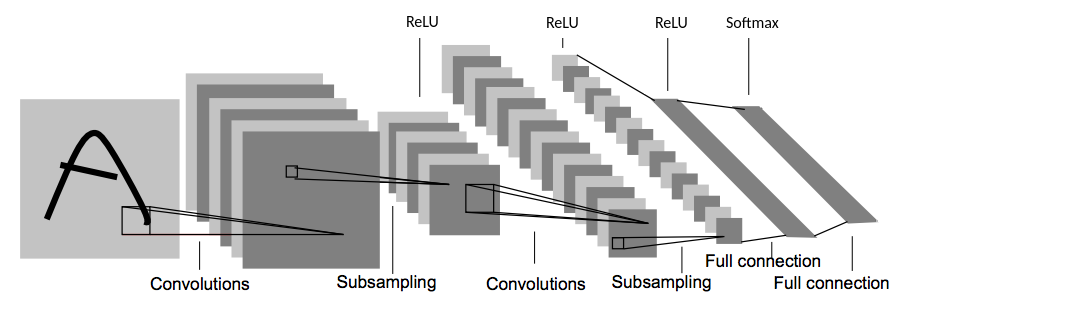
\includegraphics[scale=0.5]{chapter1/lenet5.png}
\caption{LeNet-5 \citep{lecun1989backpropagation}}
\label{fig:lenet}
\end{figure}

Another example is the VGG architecture, a very deep CNN, and was state-of-the-art in image classification in 2014 (\citeauthor{simonyan2014very}). It is depicted on \figref{fig:vgg}

\begin{figure}[htp]
\centering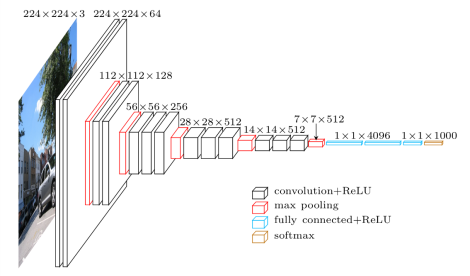
\includegraphics[scale=0.8]{chapter1/vgg16.png}
\caption{VGG-16 (\cite{simonyan2014very}, figure from~\cite{vgg})}
\label{fig:vgg}
\end{figure}

In more recent years, state-of-the-art architectures can no longer be described with a simple formalization.

%\paragraph{Generic formalization}
The former neural networks are said to be \emph{simply connected} because each layer only takes as input the output of the previous one. We'll give a more general definition after first defining branching operations.

\begin{definition}\textbf{Branching}\\
A \emph{binary branching operation} between two tensors, $x_{k_1} \Join x_{k_2}$, outputs, subject to shape compatibility, either their addition, either their concatenation along a rank, or their concatenation as a list.

A \emph{branching operation} between $n$ tensors, $x_{k_1} \Join x_{k_2} \Join \cdots \Join x_{k_n}$, is a composition of binary branching operations, or is the identity function $\id$ if $n = 1$.

Branching operations are also naturally defined on tensor-valued functions.% via their realizations.
\end{definition}

\begin{definition}\textbf{Neural network (generic definition)}\\
The set of \emph{neural network} functions $\cn$ is defined inductively as follows
\begin{enumerate}
  \item $Id \in \cn$
  \item $f \in \cn \wedge (g,h) \text{ is a layer} \wedge O_f \subset I_g \Rightarrow h \circ g \circ f \in \cn$
  \item for all shape compatible branching operations:\\
  $\quad f_1, f_2, \ldots, f_n \in \cn \Rightarrow  f_1 \Join f_2 \Join \cdots \Join f_n \in \cn$
\end{enumerate}
\label{def:nn2}
\end{definition}

\paragraph{Examples}
The neural network proposed in \citep{szegedy2015going}, called \emph{Inception}, use depth-wise concatenation of feature maps. Residual networks (ResNets, \cite{he2016deep}) make use of \emph{residual connections}, also called \emph{skip connections}, \ie an activation that is used as input in a lower level is added to another activation at an upper level, as depicted on \figref{fig:resnet}. Densely connected networks (DenseNets, \cite{huang2017densely}) have their activations concatenated with all lower level activations. These neural networks had demonstrated state of the art performances on the imagenet classification challenge \citep{deng2009imagenet}, outperforming simply connected neural networks. For example, DenseNet is depicted on \figref{fig:densenet}.
\label{par:branching_ex}

\begin{figure}[htp]
\centering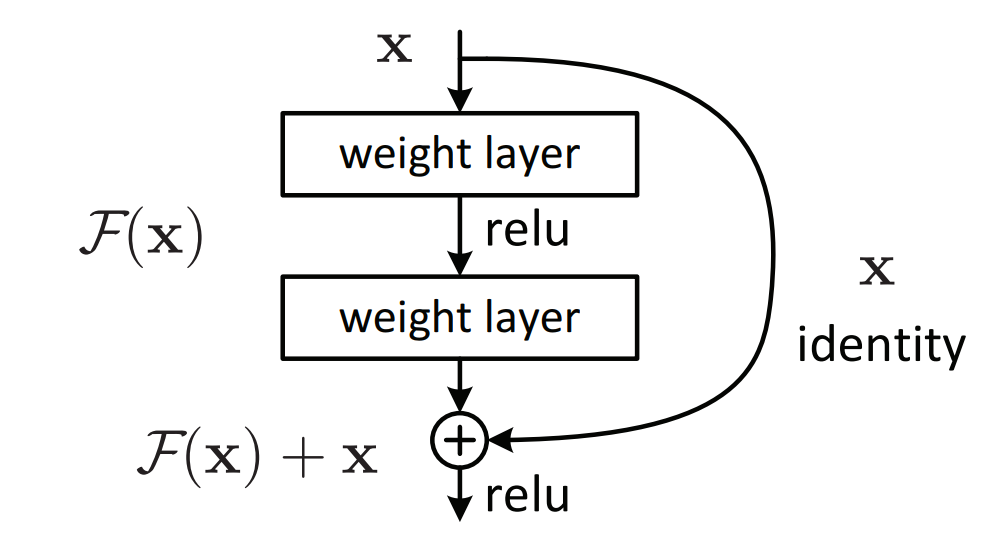
\includegraphics[scale=0.2]{chapter1/resnetmodule.png}
\caption{Module with a residual connection \citep{he2016deep}}
\label{fig:resnet}
\end{figure}

\begin{figure}[htp]
\centering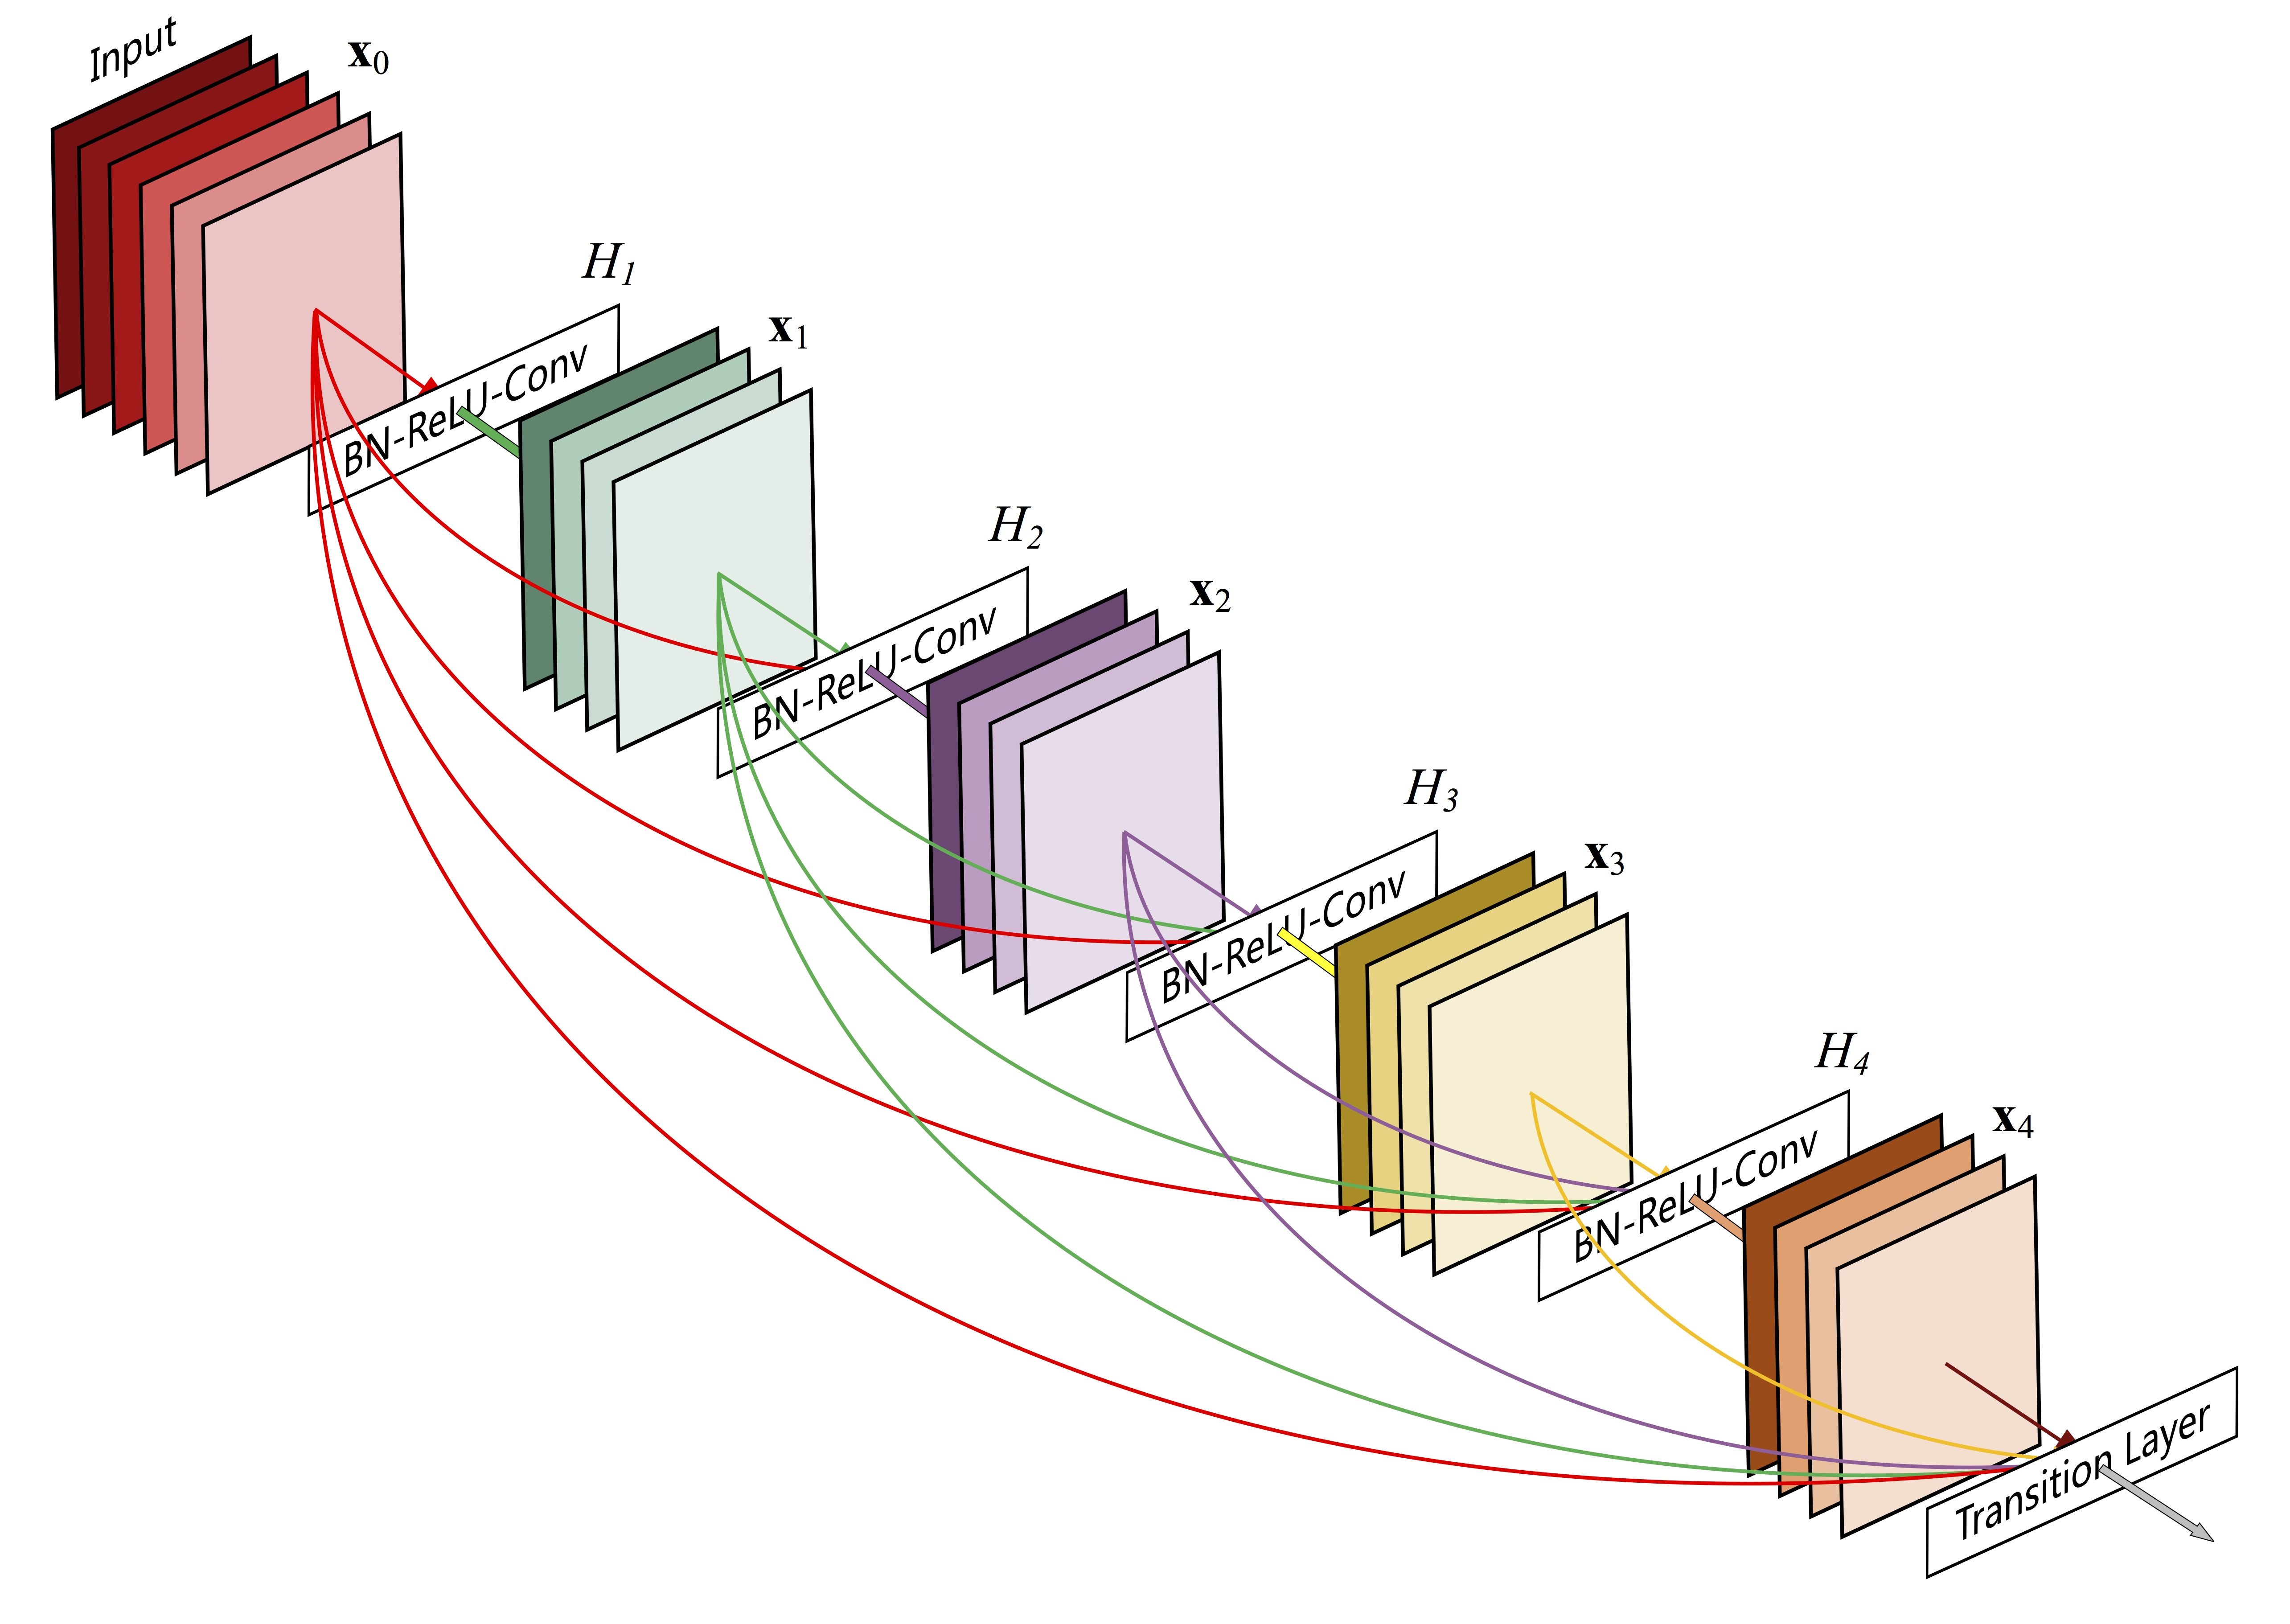
\includegraphics[scale=0.07]{chapter1/densenet.jpg}
\caption{DenseNet \citep{huang2017densely}}
\label{fig:densenet}
\end{figure}

\begin{remark}
For layer indexing convenience, we still use the simple formalization in the subsequent subsections, even though the presentation would be similar with the generic formalization.
\end{remark}

\subsection{Interpretation}
\label{sec:int}

Until now, we have formally introduced a neural network as a mathematical function. As its name suggests, such function can be indeed interpreted from a connectivity perspective \citep{lecun-87}.

\begin{definition}\textbf{Connectivity matrix}\\
Let $g$ a linear function. Without loss of generality subject to a flattening, let's suppose $I_g$ and $O_g$ are vector spaces. Then there exists a \emph{connectivity matrix}~$W_g$, such that:
\begin{gather*}
\forall x \in I_g, g(x) = W_g x
\end{gather*}
\end{definition}
We denote $W_k$ the connectivity matrix of the $k$-th layer.

\paragraph{Biological inspiration}
A \emph{neuron} is defined as a computational unit that is biologically inspired \citep{mcculloch1943logical}. Each neuron is capable of:
\begin{enumerate}[noitemsep,nolistsep]
\item receiving modulated signals from other neurons and aggregate them,
\item applying to the result an activation function,
\item passing the signal to other neurons.\\
\end{enumerate}
That is to say, each domain $\{I_{f_k}\}$ and $O_f$ can be interpreted as a layer of neurons, with one neuron for each dimension. The connectivity matrices $\{W_k\}$ describe the connections between each successive layers.
%The parameters of $\Theta_g$ are the modulation weights that characterize the connections.
A neuron is illustrated on \figref{fig:neuron}.

\begin{figure}[h!tb]
\centering
\begin{tikzpicture}[
init/.style={
  draw,
  circle,
  inner sep=2pt,
  font=\Huge,
  join = by o-latex
},
squa/.style={
  draw,
  inner sep=2pt,
  font=\Large,
  join = by -latex
},
start chain=2,node distance=13mm
]
\node[on chain=2] 
  (x2) {$x_2$};
%\node[on chain=2,join=by o-latex] 
%  {$w_2$};
\node[on chain=2,init] (sigma)
  {$\displaystyle\Sigma$};
\node[on chain=2,squa,label=above:{\parbox{2cm}{\centering activation}}]   
  {$h$};
\node[on chain=2,join=by -o] 
  {$y$};
\begin{scope}[start chain=1]
\node[on chain=1] at (0,1.5cm) 
  (x1) {$x_1$};
%\node[on chain=1,join=by o-latex] 
%  (w1) {$w_1$};
\end{scope}
\begin{scope}[start chain=3]
\node[on chain=3] at (0,-1.5cm) 
  (x3) {$x_3$};
%\node[on chain=3,label=below:Weights,join=by o-latex] 
%  (w3) {$w_3$};
\end{scope}
\node[label=above:{\centering bias}] at (sigma|-x1) (b) {};

\draw[o-latex] (x1) -- (sigma);
\draw[o-latex] (x3) -- (sigma);
\draw[o-latex] (b) -- (sigma);

\node at (1cm,1.2cm) {$w_1$};
\node at (1cm,0.2cm) {$w_2$};
\node at (1cm,-0.5cm) {$w_3$};
\node at (2.37cm,0.9cm) {$b$};

%\draw[decorate,decoration={brace,mirror}] (x1.north west) -- node[left=10pt] {Inputs} (x3.south west);
\end{tikzpicture}
\caption{A neuron}
\label{fig:neuron}
\end{figure}

\subsection{Training}
\label{sec:training}

Given an objective function $F$, training is the process of incrementally modifying a neural network $f$ upon obtaining a better approximation of $F$.
The most used training algorithms are based on gradient descent, as proposed in \citep{widrow1960adaptive}. These algorithms became popular since \citep{rumelhart1985learning}. Informally, $f$ is parameterized with initial weights that characterize its linear parts. These weights are modified step by step. At each step, a batch of samples are fed to the network, and their approximation errors sum to a loss. The weights of the network are updated in the opposite direction to their gradient with respect to that loss. If the samples are shuffled and grouped in batches, this is called \emph{Stochastic} gradient descent (SGD). Stochastic approximation \citep{robbins1985stochastic} tends to minimize effects of outliers on the training and is agnostic of the order in which the samples are fed.

%All possible realizations of $f$ through its weights draw a family $N$ which expressivity is crucial for the success of the training. The common points between $f$ and other objects of $N$ define what is called a neural network \emph{architecture}. That is

\begin{definition}\textbf{Weights}\\
Let consider the $k$-th layer of a neural network $f$. We define its weights as coordinates of a vector $\theta_k$, called the \emph{weight kernel}, such that:
\begin{gather*}
  \forall (i,j),
    \begin{cases}
      \exists p, W_k[i,j] := \theta_k[p] \\
      \text{ or } W_k[i,j] = 0
    \end{cases}
\end{gather*}
\end{definition}
A weight $p$ that appears multiple times in $W_k$ is said to be \emph{shared}. Two parameters of $W_k$ that share a same weight $p$ are said to be \emph{tied}. The number of weights of the $k$-th layer is $n_1^{(\theta_k)}$.

\paragraph{Learning}
A \emph{loss} function $\mathcal{L}$ penalizes the output $x_L = f(x)$ relatively to the approximation error $|f(x) - F(x)|$. Gradient w.r.t.~$\theta_k$, denoted $\vec{\bigtriangledown}_{\theta_k}$, is used to update the weights via an optimization algorithm based on gradient descent and a learning rate $\alpha$, that is:
\begin{gather}
\theta_k^{(\text{new})} = \theta_k^{(\text{old})} - \alpha \cdot \vec{\bigtriangledown}_{\theta_k} \left( \mathcal{L}\left( x_L, \theta_k^{(\text{old})} \right) + \ccr\left( \theta_k^{(\text{old})} \right) \right)
\end{gather}
where $\ccr$~is a regularizer, and where $\alpha$~can be a scalar or a vector and $\cdot$~can denote outer or coordinate-wise product, depending on the optimization algorithm that is used.

\paragraph{Linear complexity}
Without loss of generality, we assume that the neural network is simply connected. Thanks to the chain rule, $\vec{\bigtriangledown}_{\theta_k}$ can be computed using gradients that are w.r.t. $x_k$, denoted $\vec{\bigtriangledown}_{x_k}$, which in turn can be computed using gradients w.r.t. outputs of the next layer $k+1$, up to the gradients given on the output layer.

That is:
\begin{align}
  \vec{\bigtriangledown}_{\theta_k} & = J_{\theta_k}(x_k) \vec{\bigtriangledown}_{x_k} \\
  \begin{split}
  \vec{\bigtriangledown}_{x_k} & = J_{x_k}(x_{k+1}) \vec{\bigtriangledown}_{x_{k+1}} \\
  \vec{\bigtriangledown}_{x_{k+1}} & = J_{x_{k+1}}(x_{k+2}) \vec{\bigtriangledown}_{x_{k+2}} \\
  \quad \quad \ldots\\
  \vec{\bigtriangledown}_{x_{L-1}} & = J_{x_{L-1}}(x_{L}) \vec{\bigtriangledown}_{x_{L}}
  \label{eq:bp}
  \end{split}
\end{align}
Obtaining,
\begin{align}
  \vec{\bigtriangledown}_{\theta_k} = J_{\theta_k}(x_k) (\prod_{p=k}^{L-1} J_{x_p}(x_{p+1})) \vec{\bigtriangledown}_{x_L}
\end{align}
where $J_{\text{wrt}}(.)$ are the respective jacobians which can be determined with the layer's expressions and the $\{x_k\}$; and $\vec{\bigtriangledown}_{x_L}$ can be determined using $\mathcal{L}$, $\ccr$ and $x_L$.
This allows to compute the gradients with a complexity that is linear with the number of weights (only one computation of the activations), instead of being quadratic if it were done with the difference quotient expression of the derivatives (one more computation of the activations for each weight).

\paragraph{Backpropagation}
We can remark that \eqref{eq:bp} rewrites as
\begin{align}
  \begin{split}
  \vec{\bigtriangledown}_{x_k} & = J_{x_k}(x_{k+1}) \vec{\bigtriangledown}_{x_{k+1}} \\ 
                               & = J_{x'_k}(h(x'_k)) J_{x_k}(W_k x_k) \vec{\bigtriangledown}_{x_{k+1}}
  \end{split}
\end{align}
where $x'_k = W_k x_k$, and these jacobians can be expressed as:
\begin{align}
  \begin{split}
  J_{x'_k}(h(x'_k)) & [i,j] = \delta_i^j h'(x'_k[i])\\
  J_{x'_k}(h(x'_k)) & = I \hspace{2pt} h'(x'_k)
  \end{split}\\
  J_{x_k}(W_k x_k) & = W_k^T
\end{align}
That means that we can write $\vec{\bigtriangledown}_{x_k} = (\widetilde{h}_k \circ \widetilde{g}_k)(\vec{\bigtriangledown}_{x_{k+1}})$ such that the connectivity matrix $\widetilde{W}_k$ is obtained by transposition. This can be interpreted as gradient calculation being a \emph{back-propagation} on the same neural network, in opposition of the \emph{forward-propagation} done to compute the output.

\subsection{Some historical advances}
\label{sec:hist}

\paragraph{Universal approximation}
Early researches have shown that neural networks with one level of depth can approximate any real-valued function defined on a compact subset of~$\bbr^n$. This result was first proved for sigmoidal activations \citep{cybenko1989approximation}, and then it was shown it did not depend on the sigmoidal activations \citep{hornik1989multilayer,hornik1991approximation}.

For example, this result brings theoretical justification that objective functions exists (even though it does not inform whether an algorithm to approach it exists or is efficient).

\paragraph{Computational difficulty}
However, reaching such objective is a computationally difficult problem, which drove back interest from the field. Thanks to better hardware and to using better initialization schemes that speed up learning, researchers started to report more successes with deep neural networks \citep{hinton2006fast,glorot2010understanding} ; see \citep{bengio2009learning} for a review of this period. It ultimately came to a surge of interest in the field after a significant breakthrough on the imagenet dataset \citep{deng2009imagenet} with deep CNNs \citep{krizhevsky2012imagenet}. The use of the fast ReLU activation function \citep{glorot2011deep} as well as leveraging graphical processing units with CUDA \citep{nickolls2008scalable} were also key factors in overcoming this computational difficulty.

\paragraph{Adoption of ReLU activations}
Historically, sigmoidal and tanh activations were mostly used \citep{cybenko1989approximation, lecun1989backpropagation}. However in recent practice, the ReLU activation (first introduced as the \emph{positive part}, \cite{jarrett2009best}), become the most used activation, as it was demonstrated to be faster and to obtain better results \citep{glorot2011deep}. ReLU originated numerous variants \eg \emph{leaky rectified linear unit} \citep{maas2013rectifier}, \emph{parametric rectified linear unit} (PReLU, \cite{he2015delving}), \emph{exponential linear unit} (ELU, \cite{clevert2015fast}), \emph{scaled exponential linear unit} (SELU, \cite{Klambauer2017self}), each one having particular advantages in some applications.

\paragraph{Combatting overfitting}
Neural networks, like any other machine learning technique, may overfit. That is, a model may behave well on the training set but fails to generalize well on unseen examples. The introduction of dropout \citep{srivastava2014dropout} have helped models with more parameters to be less prone to overfitting, as dropout consists in hiding some parts of the training samples and their intermediate activations. Another good practice is to normalize per batch \citep{ioffe2015batch}.
%Dropout consists in randomly setting a certain number of neurons to zero during the training phase (compensated at test time by scaling down the whole layer). The idea is that some part of the training samples are hidden to the model, so that it cannot overfit on them.

\paragraph{Expressivity and expressive efficiency}
The study of the \emph{expressivity} (also called \emph{representational power}) of families of neural networks is the field that is interested in the range of functions that can be realized or approximated by this family \citep{haastad1991power,pascanu2013number}. In general, given a maximal error~$\epsilon$ and an objective~$F$, the more expressive is a family $N \subset \cn$, the more likely it is to contain an approximation $f \in N$ such that $d(f,F) < \epsilon$. However, if we consider the approximation $f_{min} \in N$ that have the lowest number of neurons, it is possible that~$f_{min}$ is still too large and may be unpractical. For this reason, expressivity is often studied along the related notion of \emph{expressive efficiency} \citep{delalleau2011shallow,cohen2018boosting}.
\label{par:expr}

\paragraph{Rectifier neural netowrks}
Of particular interest for the intuition is a result stating that a simply connected neural networks with only ReLU activations (a rectifier neural network) is a piecewise linear function \citep{pascanu2013number,montufar2014number}, and that conversely any piecewise linear function is also a rectifier neural network such that an upper bound of its depth is logarithmically related to the input dimension (\cite{arora2018understanding}, th. 2.1.). Their expressive efficiency have also been demonstrated compared to neural networks using threshold or sigmoid activations~\citep{pan2016expressiveness}.

\paragraph{Benefits of depth}
Expressive efficiency analysis have demonstrated the benefits of depth, \ie a shallow neural network would need an unfeasible large number of neurons to approximate the function of a deep neural network (\eg \cite{delalleau2011shallow,bianchini2014complexity,poggio2015theory,eldan2016power,poole2016exponential,raghu2016expressive,cohen2016convolutional,mhaskar2016learning,lin2017does,arora2018understanding}). This field seeks to give theoretical grounds to the practical observation that state-of-the-art architectures are getting deeper. 

\paragraph{Benefits of branching operations}
Recent works have provided rationales supporting benefits of using branching operations, thus giving justifications for architectures obtained with the generic formalization. In particular, \citep{cohen2018boosting} have analyzed the impact of residual connections used in Wavenet-like architectures \citep{van2016wavenet} in terms of expressive efficiency, using tools from the field of tensor analysis ; \citep{orhan2018skip} have empirically demonstrated that skip connections can resolve some inefficiency problems inherent of fully-connected networks (dead activations, activations that are always equal, linearly dependent sets of activations).


\subsection{Common layers}
\label{sec:layer}

\begin{definition}\textbf{Connections}\\
The set of \emph{connections} of a layer $(g,h)$, denoted $C_g$, is defined as:
\begin{gather*}
  C_g = \{(i,j), \exists p, W_g[i,j] := \theta_g[p]\}
\end{gather*}
We have $0 \leq |C_g| \leq n_1^{(W_g)} n_2^{(W_g)}$.
\end{definition}

\begin{definition}\textbf{Dense layer}\\
A \emph{dense layer} $(g,h)$ is a layer such that $|C_g| = n_1^{(W_g)} n_2^{(W_g)}$, \ie all possible connections exist. The map $(i,j) \mapsto p$ is usually a bijection, meaning that there is no weight sharing.
\end{definition}

A neural network made only of dense layers is called a Multi-Layer Perceptron (MLP, \cite{hornik1989multilayer}).

\begin{definition}\textbf{Partially connected layer}\\{}
A \emph{partially connected layer} $(g,h)$ is a layer such that $|C_g| < n_1^{(W_g)} n_2^{(W_g)}$.

A \emph{sparsely connected layer} $(g,h)$ is a layer such that $|C_g| \ll n_1^{(W_g)} n_2^{(W_g)}$.
\end{definition}

\begin{definition}\textbf{Convolutional layer}\\
A \emph{$n$-dimensional convolutional layer} $(g,h)$ is such that the weight kernel~$\theta_g$ can be reshaped into a tensor $w$ of rank $n+2$, and such that
\begin{gather*}
\left\{
\begin{array}{l}
  I_g \mbox{ and } O_g \mbox{ are tensor spaces of rank }n+1 \\
  \forall x \in I_g, g(x) = (g(x)_q = \sum\limits_p{x_p \ast^n w_{p,q}})_{\forall q}
\end{array}
\right.
\end{gather*}
where $p$ and $q$ index slices along the last ranks.
\label{def:convlayer}
\end{definition}

A neural network that contains convolutional layers is called convolutional neural network (CNN).

\begin{definition}\textbf{Feature maps and input channels}\\
The slices $g(x)_q$ are typically called \textit{feature maps}, and the slices $x_p$ are called \textit{input channels}. Let's denote by $n_o = n_{n+1}^{(O_g)}$ and $n_i =n_{n+1}^{(I_g)}$ the number of feature maps and input channels.
In other words, \defref{def:convlayer} means that for each feature maps, a convolution layer computes $n_i$ convolutions and sums them, computing a total if $n_i \times n_o$ convolutions.
\end{definition}

\begin{remark}
Note that because they are simply summed, entries of two different input channels that have the same coordinates are assumed to share some sort of relationship. For instance on images, entries of each input channel (typically corresponding to Red, Green and Blue channels) that have the same coordinates share the same pixel location.
\end{remark}

\paragraph{Benefits of convolutional layers}
Comparatively with dense layers, convolution layers enjoy a significant decrease in the number of weights. For example, an input $2 \times 2$ convolution on images with $3$-color input channels, would breed only $12$ weights per feature maps, independently of the numbers of input neurons. On image datasets, their usage also breeds a significant boost in performance compared with dense layers~\citep{krizhevsky2012imagenet}, for they allow to take advantage of the topology of the inputs while dense layers do not~\citep{lecun1995convolutional}. A more thorough comparison and explanation of their assets will be discussed in \secref{sec:cnnvsmlp}.

\paragraph{Decrease of spatial dimensions}
Given a tensor input $x$, the $n$-dimensional convolutions between the inputs channels $x_p$ and slices of a weight tensor $w_{p,q}$ would result in outputs $y_q$ of shape $n_1^{(x)} - n_1^{(w)} + 1 \times \ldots \times n_n^{(x)} - n_n^{(w)} + 1$. So, in order to preserve shapes, a padding operation must pad $x$ with $n_1^{(w)} - 1 \times \ldots \times n_n^{(w)} - 1$ zeros beforehand. For example, the padding function of the library \emph{tensorflow}~\citep{tensorflow2015-whitepaper} pads each rank with a balanced number of zeros on the left and right indices (except if $n_t^{(w)} - 1$ is odd then there is one more zero on the left).

\begin{definition}\textbf{Padding}\\
A convolutional layer with \emph{padding} $(g, h)$ is such that $g$ can be decomposed as $g = g_\text{pad} \circ g'$, where $g'$ is the linear part of a convolution layer as in \defref{def:convlayer}, and $g_\text{pad}$ is an operation that pads zeros to its inputs such that $g$ preserves tensor shapes.
\end{definition}

\begin{remark}
One asset of padding operations is that they limit the possible loss of information on the borders of the subsequent convolutions, as well as preventing a decrease in size. Moreover, preserving shape is needed to build some neural network architectures, especially for ones with branching operations \eg examples in \secref{par:branching_ex}. On the other hand, they increase memory and computational footprints.
\end{remark}

\begin{definition}\textbf{Stride}\\
A convolutional layer with \emph{stride} is a convolutional layer that computes strided convolutions (with stride $> 1$) instead of convolutions.
\end{definition}

\begin{definition}\textbf{Pooling}\\
A layer with \textit{pooling} $(g,h)$ is such that $g$ can be decomposed as $g = g' \circ g_\text{pool}$, where $g_\text{pool}$ is a pooling operation.
\end{definition}

Layers with stride or pooling downscale the signals that passes through the layer. These types of layers allows to compute features at a coarser level, giving the intuition that the deeper a layer is in the network, the more abstract is the information captured by the weights of the layer.

\paragraph{A simple result}
In two dimensions, convolutional operations can be rewritten as a matrix-vector multiplication where the matrix is Toeplitz. We show below that it is still the case in $n$~dimensions.

\begin{proposition}\textbf{Connectivity matrix of a convolution with padding}\\
A convolutional layer with padding $(g, h)$ is equivalently defined as its connectivity matrix $W_g$ being a $n_i \times n_o$ block matrix such that its blocks are Toeplitz matrices, and where each block corresponds to a couple $(p,q)$ of input channel~$p$ and feature map~$q$.
\end{proposition}

\begin{proof}
Let's consider the slices indexed by $p$ and $q$, and to simplify the notations, let's drop the subscripts $\hspace{0pt}_{p,q}$. We recall from \defref{def:convdef} that
\begin{align*}
  y &= (x \ast^n w)[j_1, \ldots, j_n] \\
 &= \displaystyle \sum_{k_1=1}^{n_1^{(w)}} \cdots \sum_{k_n=1}^{n_n^{(w)}}
    x[j_1 + n_1^{(w)} - k_1, \ldots, j_n + n_n^{(w)} - k_n] \hspace{2pt} w[k_1, \ldots, k_n] \\
 &= \displaystyle \sum_{i_1=j_1}^{j_1 + n_1^{(w)} - 1} \cdots \sum_{i_n=j_n}^{j_n + n_n^{(w)} - 1}
    x[i_1, \ldots, i_n] \hspace{2pt} w[j_1 + n_1^{(w)} - i_1, \ldots, j_n + n_n^{(w)} - i_n] \\
 &= \displaystyle \sum_{i_1=1}^{n_1^{(x)}} \cdots \sum_{i_n=1}^{n_n^{(x)}}
    x[i_1, \ldots, i_n] \hspace{2pt} \widetilde{w}[i_1, j_1, \ldots, i_n, j_n] \\
 & \text{ where } \widetilde{w}[i_1, j_1, \ldots, i_n, j_n] = \\
 & \quad \quad
 \begin{cases}
   w[j_1 + n_1^{(w)} - i_1, \ldots, j_n + n_n^{(w)} - i_n] & \text{if } \forall t, 0 \le i_t - j_t \le n_t^{(w)} - 1 \\
   0 & \text{otherwise}
 \end{cases}
\end{align*}
Using Einstein summation convention as in~\eqref{eq:indices} and permuting indices, we recognize the following tensor contraction
\begin{align}
y_{j_1 \cdots j_n} = x_{i_1 \cdots i_n} \widetilde{w} \hspace{1pt}^{i_1 \cdots i_n} \hspace{0pt}_{j_1 \cdots j_n} \label{eq:toep1}
\end{align}
Following \propref{prop:matprodeq}, we reshape~\eqref{eq:toep1} as a matrix product. To reshape $y \mapsto Y$, we use the row major order bijections $g_j$ as in~\eqref{eq:rowmajor} defined onto $\{(j_1, \ldots, j_n), \forall t, 1 \le j_t \le n_t^{(y)}\}$. To reshape $x \mapsto X$, we use the same row major order bijection $g_j$, however defined on the indices that support non zero-padded values, so that zero-padded values are lost after reshaping. That is, we use a bijection $g_i$ such that $g_i(i_1, i_2, \ldots, i_n) = g_j(i_1 - o_1, i_2 - o_2, \ldots, i_n - o_n)$ defined if and only if $\forall t, 1 + o_t \le i_t \le n_t^{(y)}$, where the $\{o_t\}$ are the starting offsets of the non zero-padded values. $\widetilde{w} \mapsto W$ is reshaped by using $g_j$ for its covariant indices, and $g_i$ for its contravariant indices. The entries lost by using $g_i$ do not matter because they would have been nullified by the resulting matrix product. We remark that $W$ is exactly the block $(p,q)$ of $W_g$ (and not of $W_{g'}$). Now let's prove that it is a Toeplitz matrix.

Thanks to the linearity of the expression~\eqref{eq:rowmajor} of $g_j$, by denoting $i'_t = i_t - o_t$, we obtain
\begin{gather}
  g_i(i_1, i_2, \ldots, i_n) - g_j(j_1, j_2, \ldots, j_n) = g_j(i'_1 - j_1, i'_2 - j_2, \ldots, i'_n - j_n)
\label{eq:toep2}
\end{gather}

To simplify the notations, let's drop the arguments of $g_i$ and $g_j$. By bijectivity of $g_j$, \eqref{eq:toep2} tells us that $g_i - g_j$ remains constant if and only if $i'_t - j_t$ remains constant for all $t$. Recall that 
\begin{gather}
  W[g_i,g_j] =
 \begin{cases}
   w[j_1 + n_1^{(w)} - i'_1, \ldots, j_n + n_n^{(w)} - i'_n] & \text{if } \forall t, 0 \le i'_t - j_t \le n_t^{(w)} - 1 \\
   0 & \text{otherwise}
 \end{cases}
\label{eq:toep3}
\end{gather}
Hence, on a diagonal of $W$, $g_i - g_j$ remaining constant means that $W[g_i,g_j]$ also remains constants. So $W$ is a Toeplitz matrix.

The converse is also true as we used invertible functions in the index spaces through the proof.
\end{proof}

\begin{remark}
Note that the proof does not hold in case there is no padding. This is due to border effects when the index of the $n$\powth rank resets in the definition of the row-major ordering function $g_j$ that would be used. Indeed, under appropriate definitions, the matrices could be seen as almost Toeplitz.
\end{remark}

This proposition provides an equivalent-characterization of convolutional layers by their connectivity matrix. Therefore, a first avenue to define convolutions on graph signals could be to define them with the connectivity matrix being as in this characterization. However, the Toeplitz property implies that the dimensions have a specific order, which is not possible when dimensions correspond to vertices of a graph. This is because permuting the order of the vertices wouldn't change the graph, but would change the connectivity matrix (which cannot be Toeplitz for every ordering).

%\subsection{Examples of regularization}

% \paragraph{Overfitting}
% \todo{}

% A layer with \textit{dropout} $(g,h)$ is such that $h = h_1 \circ h_2$, where $(g,h_2)$ is a layer and $h_1$ is a dropout operation~\citep{srivastava2014dropout}. When dropout is used, a certain number of neurons are randomly set to zero during the training phase, compensated at test time by scaling down the whole layer. This is done to prevent overfitting.

% \subsection{Examples of architecture}
% \label{sec:nn_arch}

% \todo{rephrase}

% A multilayer perceptron (MLP)~\citep{hornik1989multilayer} is a neural network composed of only dense layers.
% A convolutional neural network (CNN)~\citep{lecun1998gradient} is a neural network composed of convolutional layers.

% Neural networks are commonly used for machine learning tasks. For example, to perform supervised classification, we usually add a dense output layer $s=(g_{L+1},h_{L+1})$ with as many neurons as classes. We measure the error between an output and its expected output with a discriminative loss function $\mathcal{L}$. During the training phase, the weights of the network are adapted for the classification task based on the errors that are back-propagated~\citep{hornik1989multilayer} via the chain rule and according to a chosen optimization algorithm (\eg \cite{bottou2010large}).
\newpage
  \section{Deep learning on graphs}

Deep learning algorithms have been particularly successful for datasets of signals defined on regular domains such as images or time series. One key ingredient of their success is the use of convolutions. However, classical convolutions are only defined on euclidean domains, so that extending deep learning on non-euclidean domains is not straightforward. The most general way to represent a non-euclidean domain is through a graph \ie as points (the vertices) and relations between them (the edges). This field also comprises the study of deep learning on manifolds (\ie locally euclidean domains). The field of deep learning on graphs or manifolds have been called recently Geometric Deep Learning \citep{bronstein2017geometric}. In this manuscript, we are only interested in deep learning on graphs.

\subsection{Graph and signals}

We present the vocabulary, notation and conventions we will employ for graphs and signals.

\begin{definition}\textbf{Graph}\\
A \emph{graph} $G$ is a couple of countable vertex and edge sets $\langle V,E \rangle$ \st $E \subset V^2$.
\end{definition}

The terms \emph{vertex} and \emph{node} are used interchangeably. Additionaly, we consider that a graph is always \emph{simple} \ie no two edges share the same set of vertices.
Unless stated otherwise, a graph is undirected, \ie $(u,v)$ and $(v,u)$ refer to the same edge. When it's not the case, it is called a \emph{digraph}.
We define the relation $u \sim v \Leftrightarrow (u,v) \in E$. We precise the graph if needed over the symbol $\overset{G}\sim$.
A \emph{path} is a sequence $v_1 \sim \cdots \sim v_r$. It is said to be \emph{simple} if its vertices are distincts, except possibly for the first and last. A graph is said to be \emph{connected} if there exists a path from any vertex to any other vertex.
We define the \emph{neighborhood} of a vertex as $\cn_u = \{v \in V, u \sim v\}$. For digraphs, it is equal to the union of the \emph{in}- and \emph{out}-neighborhoods. We only consider graphs without isolated vertex (a vertex with an empty neighborhood).
We also only consider \emph{weighted} graphs. That is, a graph $\gve$ is associated with a weight mapping $w: V^2 \to \bbr+$ \st $w(u,v) = 0 \Leftrightarrow u \nsim v$.
If $G$ is finite, its \emph{adjacency matrix} $A \in \bbr^{V \times V}$ is defined \wrt to a vertex ordering $V = \{v_1, \ldots, v_n\}$ as $A[i,j] = w(v_i,v_j)$. \figref{fig:graph} illustrates an example of a graph and its adjacency matrix.

\begin{figure}[h!tp]
\centering
\begin{tikzpicture}
\draw (0,0) -- (4,0) -- (4,4) -- (0,4) -- (0,0);
\node at (2,2){placeholder};
\end{tikzpicture}
\caption{Example of a graph}
\label{fig:graph}
\end{figure}

The \emph{order} of $G$ is equal to its number of vertices, possibly infinite.
The \emph{degree} of a vertex $v$ is equal to the number of edges it is attached to.
For digraphs the degree is the sum of the \emph{in}- and \emph{out}-degrees.
The \emph{degree} of $G$ refers to its max degree.
$G$ is said to be \emph{degree-regular} if all its vertices have the same degree.
If it is finite, its \emph{degree matrix} $D$ (\wrt to a vertex ordering $V = \{v_1, \ldots, v_n\}$) is the diagonal matrix for which the diagonal entry corresponding to a vertex is the sum of the weights of the edges it is part of.
Its \emph{laplacian matrix} $L$ is the substraction $L = D-A$, which can be \emph{normalized} $L = I - D^{-\frac{1}2}AD^{-\frac{1}2}$, \emph{left-normalized} $L = I - D^{-1}A$, or \emph{right-normalized} $L = I - AD^{-1}$.
A subgraph of $G$ induced by a subset $U \subset V$ is the graph with vertex and edge set restricted by $U$. The \emph{complement} graph $G^C$ shares the same vertex set but $u \overset{G^C}\sim v \Leftrightarrow u \overset{G}\nsim v$.
A \emph{complete} graph is such that there exists an edge between any two vertices.

% \begin{definition}\textbf{Grid graph}\\
% A \emph{grid graph} $\gve$ is 
% such that $V \cong \bbz^2$, $v_1 \sim v_2 \Rightarrow \|v_2 -v_1\|_\infty \in \{0, 1\}$ and either one of the following is true:
% \begin{gather*}
% \left\{
%   \begin{array}{l}
%     (i_1,j_1) \sim (i_2,j_2) \Leftrightarrow |i_2 - i_1| \XOR |j_2 - j_1| \quad \text{($4$ neighbours)}\\
%     (i_1,j_1) \sim (i_2,j_2) \Leftrightarrow |i_2 - i_1| \AND |j_2 - j_1| \quad \text{($4$ neighbours)}\\
%     (i_1,j_1) \sim (i_2,j_2) \Leftrightarrow |i_2 - i_1| \OR |j_2 - j_1| \quad \text{($8$ neighbours)}
%   \end{array}
% \right.
% \end{gather*}

% A \emph{(rectangular) grid graph} of size $n \times m$ is the subgraph of a grid graph induced by $\llbracket 1, n \rrbracket \times \llbracket 1, m \rrbracket$. A \emph{square grid graph} is a rectangular grid graph of square size.
% \end{definition}

\begin{definition}\textbf{Grid graph}\\
Let a graph $\gve$ such that the expression $u \sim v \Leftrightarrow \|u-v\|_1 = 1$ makes sense. $G$ can be called:
\begin{itemize}[nolistsep,noitemsep]
\item a \emph{grid graph} if $V = \bbz^2$
\item a \emph{finite grid graph} if $\exists (n,m) \in \bbz^2, V = \llbracket 1, n \rrbracket \times \llbracket 1, m \rrbracket$
\item a \emph{circulant grid graph} if $\exists (n,m) \in \bbz^2, V = \bbz /n \bbz \times \bbz /m \bbz$
\end{itemize}
\end{definition}

\begin{definition}\textbf{Bipartite graph}\\
A graph is called \emph{bipartite} if its vertex set is a disjoint union $V = V_1 \cup V_2$ \st $$u \sim v \Rightarrow (u,v) \in V_1 \times V_2 \vee (u,v) \in V_2 \times V_1$$
\end{definition}

If it is finite, its \emph{bipartite-adjacency} matrix $A \in \bbr^{V_1 \times V_2}$ is a rectangular matrix defined \wrt to a vertex ordering $V_1 = \{u_1, \ldots, u_n\}$, $V_2 = \{v_1, \ldots, v_n\}$ and weight mapping $w$ as $A[i,j] = w(u_i,v_j)$.

\begin{definition}\textbf{Signal}\\
A \emph{signal} on $V$, $s \in \cs(V)$, is a function $s: V \rightarrow \bbr$.
The \emph{signal space} $\cs(V)$ is the linear space of signals on $V$.
\end{definition}

\begin{remark}
In particular, a vector space, and more generally a tensor space, are finite-dimensional signal spaces on any of their bases.
\end{remark}

A \emph{graph signal} on a graph $\gve$ is a signal on its vertex set $V$. We denote by $\cs(G)$ or $\cs(V)$ the graph signal space. $G$ can be referred as the \emph{underlying structure} of $\cs(V)$.
An \emph{entry} of a signal $s$ is an image by $s$ of some $v \in V$ and we denote $s[v]$. If~$v$~is represented by an $n$-tuple, we can also write $s[v_1, v_2, \ldots, v_n]$.
The \emph{support} of a signal $s \in \cs(V)$ is the subset $\supp(s) \subset V$ on which $s \neq 0$.
For spaces of signals that aren't real-valued, their codomain~$\bbe$ is precised in the subscript~$\cs_{\bbe}(V)$.

\subsection{Learning tasks}

\todo{add example of datasets descriptions}

There are many tasks related to deep learning on graphs.%:
% \begin{itemize}[nolistsep,noitemsep]
%   \item supervised classification of graph signals
%   \item supervised classification of graphs
%   \item semi-supervised classification of node signals
%   \item semi-supervised representation learning of nodes
% \end{itemize}

\paragraph{Supervised classification of graph signals}
This is the classical application of deep learning transposed to graph signals, rather than image or audio signals. It is the principled targeted task we will have in mind in the course of the remainder of this manuscript. Given a graph $\gve$ and an input signal $x \in \cs(G)$ the goal is to classify~$x$. If there are~$c$ possible classes, a neural network~$f$ outputs a vector $y = f(x)$ of dimension~$c$, and its dimension with the biggest weight determines the predicted class. Indeed, a standard MLP can be trained on a dataset of graph signals. However, an MLP wouldn't take the graph structure $G$ into consideration. By similarity with CNNs that leverage the grid structure of images to achieve better performances than MLPs, a challenge is to define a neural network on graph signals that can leverage~$G$. We review some models from the litterature in \secref{sec:spec} and in \secref{sec:vert}. We develop an algebraic understanding in \chapref{chap:2} of why and how they should work, and also propose our own models and point of view in \chapref{chap:3}.

\paragraph{Semi-supervised classification of nodes}
This task is in some way obtained from a transposed perspective of the previous one. Given a dataset of graph signals, represented as a matrix $X \in \bbr^{n \times N}$, where the rows represent the nodes, and the columns represent the signals, the goal is to classify the nodes. This amounts to classify the rows, whereas the previous task amounts to classify the columns. As opposed to the previous one, this task is \emph{transductive} \ie node data from the test set are available during training (but their labels are not), and it is \emph{semi-supervised} \ie some node labels of the train set are unknown. This allows to learn on much more data than if we were restricted to labeled data. In this task, the edges connect learning samples, however in the previous one, the edges were connecting features of learning samples. This is this edge relationship between learning samples that renders the semi-supervised approach possible. This task have received much more attention than the previous one in the recent litterature. We explain why in \secref{sec:spec}.

\paragraph{Other learning tasks}
In this manuscipt, we are less interested in other deep learning tasks related to graphs, so we briefly discuss them here. One is supervised classification of graphs, which is different than classifying graph signals. Examples include \citep{niepert2016learning,tixier2017classifying}. Another interesting task is the semi-supervised representation learning of nodes, which tackles the challenge to learn a linear representation of nodes. A common approach, derived from word2vec \citep{mikolov2013efficient,mikolov2013distributed}, is called node2vec \citep{grover2016node2vec}, and was later improved in graphSAGE \citep{hamilton2017inductive}. A review on this subject is done by \cite{hamilton2017representation}.

\subsection{Spectral methods}
\label{sec:spec}

Spectral methods are based on spectral graph theory \citep{chung1996spectral} which aims at characterizing structral properties of a graph $\gve$ through the eigenvalues of the laplacian matrix $L$. In particular, since it is hermitian, it admits a complete set of normalized eigenvectors. By fixing a normalized eigenvector basis ordered in the rows of $U$ (by ascending eigenvalues), $U$ is used to define the \emph{Graph Fourier Transform} (GFT) of a signal $s \in \cs(G)$ \citep{shuman2013emerging}, and the conjugate-transpose $U^*$ defines the inverse GFT. We write
\begin{align}
\widehat{s} &= Us\\
\widetilde{s} &= U^*s
\end{align}

\begin{remark}
The GFT extends the notion of \emph{Discrete Fourier Transform} (DFT) to general graphs, since that for circulant grid graphs $U$ can be the DFT matrix.
\end{remark}

By analogy with the convolution theorem, a convolution can be defined as pointwise multiplication, denoted $\cdot$, in the spectral domain of the graph \citep{hammond2011wavelets}. For $s, g \in \cs(G)$, we have:
\begin{gather}
s \ast g = \widetilde{\widehat{s} \cdot \widehat{g}} \label{eq:sc}
\end{gather}

This expression can be used to define convolutional layers and spectral CNNs on graphs. However, \cite{bruna2013spectral} pointed out that \eqref{eq:sc} would generate filters with $\co(n)$ weights, where $n$ is the order of $G$. So they proposed to learn filters $\theta$ with only $\co(1)$ weights and then to smoothly interpolate the remaining weights as $g = K \theta$, where $K$ is a linear smoother matrix. They motivate their construction by the fact that smooth multipliers in the spectral domain should simulate local operations in the vertex domain. To elaborate a bit on this, note that we have:
\begin{align}
Ls[u] &= \displaystyle\sum_{v \in V} w(u,v)(s[u] - s[v])
\end{align}
And so,
\begin{align}
s^TLs &= \displaystyle\sum_{u \in V}\sum_{v \in V} w(u,v)s[u](s[u] - s[v])\nonumber\\
&= \displaystyle \frac{1}2\sum_{u \in V}\sum_{v \in V} w(u,v)s[u](s[u] - s[v]) + \frac{1}2\sum_{v \in V}\sum_{u \in V} w(v,u)s[v](s[v] - s[u])\nonumber\\
&=  \displaystyle\sum_{u \in V}\sum_{v \in V} \frac{w(u,v)}2(s[u] - s[v])^2 \label{eq:smooth}
\end{align}
That is, $s^TLs$ is some sort of measure of \emph{smoothness} of the signal $s$, penalized by the weights $w$. The bigger is $w(u,v)$, the closest $s(u)$ and $s(v)$ must be to lower the smoothness \eqref{eq:smooth}. Since $L$ is symmetric, its eigenvalues are non-negative real numbers, and $U$ diagonalizes $L$ as $\Lambda = ULU^*$. Denote $(\lambda_i)_i$ the eigenvalues, the smoothness measure rewrites:
\begin{align}
s^TLs = \widehat{s}^*\Lambda\widehat{s} = \displaystyle\sum_{i=1}^n \lambda_i \widehat{s}[i]^2
\end{align}
Therefore, as they pointed out, smoothness of $s$ can be read off the coordinates of $\hat{s}$, like for the DFT. Moreover, spectral multipliers modulate its smoothness, and decay in the spectral domain is related to smoothness in the vertex domain. But contrary to their conjecture, smoothness in the spectral domain is not necessary related to decay is the vertex domain (and so to some form of locality). For instance, since the laplacian $L^C$ of the complement graph $G^C$ commutes with $L$, it can share the same eigenvector basis $U$, and thus define the same GFT, but their notion of locality in the vertex domain are opposed. Another drawback is that this method requires computing the GFT which complexity is at least $\co(n^2)$ as there is no equivalent of the Fast Fourier Transform (FFT) on graphs, so the authors suggest to use a lower number of eigenvectors $d < n$ from the laplacian eigenbasis.

Then, \cite{defferrard2016convolutional} remedy to these issues by proposing an approximate formulation based on the Chebychev polynomials, denoted by $(T_i)_i$, where $i$ is the polynomial order.
That is, their proposed approximate filters are in the form
\begin{gather}
g_\theta(L) = \sum_{i=0}^k \theta[i] \h{2} T_i(\widetilde{L})
\end{gather}
where $\widetilde{L} = \frac{\lambda_{\max}}2L - I_n$ is the scaled normalized laplacian with eigenvalues lying in the range $[-1,1]$. $g_\theta(L)$ are spectral multipliers since we have:
\begin{align}
g_\theta(L)s &= g_\theta(U^*\Lambda U)s
= U^* g_\theta(\Lambda) Us\nonumber\\
&= \widetilde{g_\theta(\Lambda) \textbf1} \ast s
\end{align}

These filters enjoy locality properties, they contain $\co(1)$ weights, and their complexity is $\co(n)$ when rows of $L$ are sparse. The use of truncated Chebychev exapansion \citep{hammond2011wavelets} ensures that in theory any set of spectral multipliers can be approximated. Also, since they are laplacian polynomials, some authors would argue that these filters are transferable from one graph to another. From a combinatorial point of view this is true. However there is no reason that spectral multipliers from a spectral domain make sense in another one, and there are no experiment in the literature to support the hypothesis. On the other hand, \citep{yi2016syncspeccnn} (which don't use polynomial filters) fix a canonical spectral base in order to synchronize every spectral domains. Their idea is to learn a warping from any eigenbasis to the canonical one, prior to performing spectral multiplication, in the manner of spatial transformer networks (STN) \cite{jaderberg2015spatial}).

However, it is hard to evaluate if a model performs well on the task of supervised classification of graph signals, because there are not much known datasets in the litterature for which the given graph domain holds enough information.

For example, \citeauthor{defferrard2016convolutional} built a graph signal dataset from a text categorization dataset called 20NEWS \citep{joachims1996probabilistic}. Each text is represented as a word2vec vector, and features are linked by edges with their nearest neighbors. However, their model (ChebNet32) fails to surpass Multinomial Naive Bayes (MNB). Moreover, even though they report that their model beat MLPs, our experiments show the contrary. In results we report in \tabref{tab:20}, we see that a lighter MLP, composed of a single Fully-Connected~(FC) layer with ReLU and 20\% dropout outperforms ChebNet32. We replicated their preprocessing phase from the code on their github repository and averaged our results on 10 runs of 20 epochs.

\begin{table}[H]
  \caption{Accuracies on 20NEWS}
  \begin{center}
    \bgroup
    \def\arraystretch{1.5}%  1 is the default, change whatever you need
    \begin{tabular}{|c|c|c|c|c|}
      \hline
      MNB & FC2500 & FC2500-FC500 & ChebNet32 & FC500\\
      \hline
      68.51\%$^a$ & 64.64\%$^a$ & 65.76\%$^a$ & 68.26\%$^a$ & \textbf{71.46}$\pm$0.08\%$^b$\\
      \hline
    \end{tabular}
    \egroup
  \end{center}
\begin{flushleft}
\footnotesize{
$^a$ As reported in \cite{defferrard2016convolutional}\\
$^b$ From our experiments.
}
\end{flushleft}
  \label{tab:20}
\end{table}

Despite the significant theoretical contribution, this negative result stresses out the importance of the practical graph used to support the convolution, a point that they also discussed. \cite{henaff2015deep} proposed supervised graph estimation techniques, but a better graph signal dataset would be one that come with an already suitable graph, that of current literature is still lacking.

On the other hand, attention in the domain has shifted toward the task of semi-supervised classification of nodes, where good datasets are not lacking. For example, \cite{levie2017cayleynets} mainly demonstrate the usefulness of their model on these type of tasks. They define polynomial filters, for which Chebychev filters are a special case, that are capable to specialize in narrow bands of frequency in the spectral domain.

Another spectral avenue consists in using wavelets defined in the graph spectral domain \citep{hammond2011wavelets}, in order to build a scattering network \citep{bruna2013invariant,chen2014unsupervised}. This idea have been exploited recently by \cite{zou2018Graph} then by \cite{gama2018Diffusion}.

\subsection{Vertex-domain methods}
\label{sec:vert}

As their name suggests, vertex-domain methods operates directly on the vertices of the graph. These works were originally motivated by chemistry datasets~\citep{duvenaud2015convolutional,kearnes2016molecular}. Convolution is defined as a function $f$ of the kernel weights $\theta$ and neighboring vertices (contained in the local receptive field $\ccr(v)$), usually based on dot products. That is
\begin{gather}
y[v] = f_\theta\left(\{u \in \ccr(v)\}\right)
\end{gather}
As such, it retains the property of being localized and of sharing weights. But there remains the need to specify how the shared weights are allocated in this local receptive field~\citep{vialatte2016generalizing}. This allocation can depend on \eg an arbitrary order~\citep{niepert2016learning}, on the number of hops~\citep{atwood2016diffusion,du2017topology}, on both vertices and their neighbors~\citep{monti2016geometric,simonovsky2017dynamic}, on a random walk \citep{hechtlinger2017generalization}, on another learned kernel~\citep{vialatte2017learning}, on an attention mechanism~\citep{velickovic2017graph,lee2018attention}, on pattern identification~\citep{sankar2017motif}, or on translation identification~\citep{pasdeloup2017convolutional}. All these methods differ in the function~$f$, but in the end, their definition highly overlap. That is why some authors have proposed unified frameworks~\citep{gilmer2017neural}.

In particular, \cite{kipf2016semi} were first to transpose ChebNet to the task of semi-supervised node classification. Chebychev filters then take a form that is interpretable in the vertex domain, which is
\begin{gather}
Y = \displaystyle\sum_{i=0}^k T_i(\widetilde{L}) X \Theta
\end{gather}
where $X \in \bbr^{n \times N}$, $\Theta \in \bbr^{N \times M}$, $n$ is the number of nodes, $N$ is the number of input channels (features per node), and $M$ is the number of output feature maps. On the left, powers of $\widetilde{L}$ diffuse the graph signal $X$ to share node information. On the right, $\Theta$ maps the diffused signals to another representation. So in essence, this formulation is more a vertex-domain method. They found that the best performing filters were expressed in a simplified form
\begin{gather}
Y = \widetilde{A} X \Theta
\end{gather}
where $\widetilde{A}$ is the normalized adjacency matrix of the graph to which self-loops are added. They called the architecture composed with these simple filters a Graph Convolution Network (GCN). Similiarly, $AX$ shares node information via the edges of the graph and $\Theta$ makes the model learns. This fomulation attracted a lot of research attention and was, in particular, extended with attention mechanism (no pun intended), inspired from the field of neural machine translation \citep{bahdanau2014neural}. Attention can be learned toward which input feature map is most useful \citep{velickovic2017graph}, or which neighboring vertex is \citep{lee2018attention}. Works extending GCN are numerous in recent days (\eg \cite{niepert2018towards}). We don't cover them since their novelty compared to GCN is limited.

%todo{extend ?}\newpage

%
% Chapter 2
%

\setcounter{chapter}{1}
\chapter{Convolutions on graph domains}\label{chap:2}
In this section, we present notions related to our domains of interest. In particular, for tensors we give original definitions that are more appropriate for our study. In the neural network's section, we present the concepts necessary to understand the evolution of the state of the art research in this field. In the last section, we present graphs for their usage in deep learning.

Vector spaces considered in what follows are assumed to be finite-dimensional and over the field of real numbers $\bbr$.\newpage
\vfill\minitoc\newpage

% body
\section{Analysis of the classical convolution}

In this section, we are exposing a few properties of the classical convolution that a generalization to graphs would likely try to preserve. For now let's consider a graph $G$ agnostically of its edges \ie $G \cong V$ is just the set of its vertices.

\subsection{Properties of the convolution}

Consider an edge-less grid graph \ie $G \cong \bbz^2$. By restriction to compactly supported signals, this case encompass the case of images.

\begin{definition}\textbf{Convolution on $\cs(\bbz^2)$}\\
Recall that the (discrete) convolution between two signals $s_1$ and $s_2$ over $\bbz^2$ is a binary operation in $\cs(\bbz^2)$ defined as:
\begin{align*}
\forall (a,b) \in \bbz^2, (s_1 \ast s_2) [a,b] & = \displaystyle \sum_i \sum_j s_1[i,j] \h{2} s_2[a-i, b-j]
\end{align*}
\end{definition}

\begin{definition}\textbf{Convolution operator}\\
A \emph{convolution operator} is a function of the form $f_w: x \mapsto x \ast w$, where $x$ and $w$ are signals of domains for which the convolution $\ast$ is defined. When $\ast$ is not commutative, we differentiate the \emph{right-action} operator $x \mapsto x \ast w$ from the \emph{left-action} one $x \mapsto w \ast x$.
\end{definition}

The following properties of the convolution on $\bbz^2$ are of particular interest for our study.

\paragraph{Linearity}
Operators produced by the convolution are linear. So they can be used as linear parts of layers of neural networks.

\paragraph{Locality and weight sharing}
When $w$ is compactly supported on $K$, an impulse response $f_w(x)[a,b]$ amounts to a $w$-weighted aggregation of entries of $x$ in a neighbourhood of $(a,b)$, called the \emph{local receptive field}.

\paragraph{Commutativity}
The convolution is commutative. However, it won't necessarily be the case on other domains.

\paragraph{Equivariance to translations}
Convolution operators are equivariant to translations. Below, we show that the converse of this result also holds with \propref{prop:equi}.

\subsection{Characterization on grid graphs}

Let's recall first what is a transformation, and how it acts on signals.

\begin{definition}\textbf{Transformation}\\
A \emph{transformation} $f: V \rightarrow V$ is a function with same domain and codomain. The set of transformations is denoted $\Phi(V)$. The set of bijective transformations is denoted $\Phi^*(V) \subset \Phi(V)$.
\end{definition}

In particular, $\Phi^*(V)$ forms the symmetric group of $V$ and can move signals of $\cs(V)$ by linear extension of its group action.

\begin{lemma}\textbf{Extension to $\cs(V)$ by group action}\\
A bijective transformation $f \in \Phi^*(V)$ can be extended linearly to the signal space $\cs(V)$, and we have:
\begin{gather*}
\forall s \in \cs(V), \forall v \in V, f(s)[v] = s[f^{-1}(v)]
\end{gather*}
\end{lemma}
\begin{proof}
Let $s \in \cs(V), f \in \Phi^*(V), L_f \in \cl(\cs(V))$ \st $\forall v \in V, L_f(\delta_v) = \delta_{f(v)}$. Then, we have:
\begin{align*}
L_f(s) & = \displaystyle\sum_{v \in V} s[v] \h{2} L_f(\delta_v)\\
       & = \displaystyle\sum_{v \in V} s[v] \h{2} \delta_{f(v)}\\
\text{So, }
\forall v \in V, L_f(s)[v] & = s[f^{-1}(v)]
\end{align*}
\label{lem:ext}
\end{proof}

% In case $f \in \Phi^*(V)$, it can act on $\cs(V)$ through the linear operator $$ defined as:
% \begin{gather*}
% \forall s \in \cs(V), \forall v \in V, f(s)[v] := L_f s[v] = s[f^{-1}(v)]
% \end{gather*}
% \ie an entry of a transformed signal is obtained by doing a lookup of the entry of the original signal.

% In case $f \notin \Phi^*(V)$, we can still define $L_f \in \cl(\cs(V))$, however we need to linearly aggregate the entries on the fibers:
% \begin{gather*}
% \forall s \in \cs(V), \forall v \in V, f(s)[v] := L_f s[v] = \agg\{s[u], u \in f^{-1}\{v\}\}
% \end{gather*}
% where $\agg$ can be for example the sum, the average, or the max, and $\agg(\emptyset) = 0$.

We also recall the formalism of translations.

\begin{definition}\textbf{Translation on $\cs(\bbz^2)$}\\
A translation on $\bbz^2$ is defined as a transformation $t \in \Phi^*(\bbz^2)$ such that
\begin{gather*}
\exists (a,b) \in \bbz^2, \forall (x,y) \in \bbz^2, t(x,y) = (x+a,y+b)
\end{gather*}
It also acts on $\cs(\bbz^2)$ with the notation $t_{a,b}$ \ie
\begin{gather*}
\forall s \in \cs(\bbz^2), \forall (x,y) \in \bbz^2, t_{a,b}(s)[x,y] = s[x-a, y-b]
\end{gather*}
For any set $E$, we denote by $\ct(E)$ its translations if they are defined.
\end{definition}

The next proposition fully characterizes convolution operators with their translational equivariance property. This can be seen as a discretization of a classic result from the theory of distributions~\citep{schwartz1957theorie}.

\begin{proposition}\textbf{Characterization of convolution operators on $\cs(\bbz^2)$}\\
On real-valued signals over $\bbz^2$, the class of linear transformations that are equivariant to translations is exactly the class of convolutive operations \ie
\begin{gather*}
\exists w \in \cs(\bbz^2), f = . \ast w \Leftrightarrow
\begin{cases}
 f \in \cl(\cs(\bbz^2))\\
 \forall t \in \ct(\cs(\bbz^2)), f \circ t = t \circ f
\end{cases}
\end{gather*}
\label{prop:equi}
\end{proposition}

\begin{proof}
The result from left to right is a direct consequence of the definitions:
\begin{align}
\forall s \in \cs(\bbz^2), \forall s' \in \cs(\bbz^2), & \forall (\alpha, \beta) \in \bbr^2,\forall (a,b) \in \bbz^2,\nonumber\\
 %f_w(s)[a,b] & = \displaystyle \sum_i \sum_j s[i,j] \h{2} w[a-i, b-j] \tag{definition}\\
 f_w(\alpha s + \beta s')[a,b] & = \displaystyle \sum_i \sum_j (\alpha s + \beta s')[i,j] \h{2} w[a-i, b-j]\nonumber\\
 & = \alpha f_w(s)[a,b] + \beta f_w(s')[a,b] \tag{linearity}\\
\forall s \in \cs(\bbz^2), \forall (\alpha, \beta) \in \bbz^2, & \forall (a,b) \in \bbz^2,\nonumber\\
f_w \circ t_{\alpha,\beta} (s)[a,b] & = \displaystyle \sum_i \sum_j t_{\alpha,\beta}(s)[i,j] \h{2} w[a-i, b-j]\nonumber\\
 & = \displaystyle \sum_i \sum_j s[i - \alpha,j - \beta] \h{2} w[a-i, b-j]\nonumber\\
 & = \displaystyle \sum_{i'} \sum_{j'} s[i',j'] \h{2} w[a - i' - \alpha, b - j'- \beta]\label{eq:bij}\\
 & = f_w (s)[a - \alpha,b - \beta]\nonumber\\
 & = t_{\alpha,\beta} \circ f_w (s)[a,b] \tag{equivariance}
\end{align}
Now let's prove the result from right to left.

Let $f \in \cl(\cs(\bbz^2))$, $s \in \cs(\bbz^2)$. We suppose that $f$ commutes with translations. Recall that $s$ can be linearly decomposed on the infinite family of dirac signals:
\begin{gather*}
s = \displaystyle \sum_i \sum_j s[i,j] \h{2} \delta_{i,j} \text{, where }
\delta_{i,j}[x,y] = \begin{cases} 1 & \text{if } (x,y) = (i,j)\\ 0 & \text{otherwise} \end{cases}
\end{gather*}
By linearity of $f$ and then equivariance to translations:
\begin{align*}
f(s) & = \displaystyle \sum_i \sum_j s[i,j] \h{2} f(\delta_{i,j})\\
 & = \displaystyle \sum_i \sum_j s[i,j] \h{2} f \circ t_{i,j} (\delta_{0,0})\\
 & = \displaystyle \sum_i \sum_j s[i,j] \h{2} t_{i,j} \circ f (\delta_{0,0})
\end{align*}
By denoting $w = f (\delta_{0,0}) \in \cs(\bbz^2)$, we obtain:
\begin{align}
\forall (a,b) \in \bbz^2, f(s)[a,b] & = \displaystyle \sum_i \sum_j s[i,j] \h{2} t_{i,j}(w)[a,b] \label{eq:conv}\\
 & = \displaystyle \sum_i \sum_j s[i,j] \h{2} w[a-i, b-j] \nonumber\\
\text{\ie } f(s) & = s \ast w \nonumber
\end{align}
\end{proof}

\subsection{Usefulness of convolutions in deep learning}
\label{sec:cnnvsmlp}

\paragraph{Equivariance property of CNNs}
In deep learning, an important argument in favor of CNNs is that convolutional layers are equivariant to translations. Intuitively, that means that a detail of an object in an image should produce the same features independently of its position in the image.

\paragraph{Lossless superiority of CNNs over MLPs}
The converse result, as a consequence of~\propref{prop:equi}, is never mentioned in deep learning literature. However it is also a strong one. For example, let's consider a linear function that is equivariant to translations. Thanks to the converse result, we know that this function is a convolution operator parameterized by a weight vector $w$, $f_w : . \ast w$. If the domain is compactly supported, as in the case of images, we can break down the information of $w$ in a finite number $n_q$ of kernels $w_q$  with small compact supports of same size (for instance of size $2 \times 2$), such that we have $f_w = \sum_{q \in \seq{n_q}} f_{w_q}$. The convolution operators $f_{w_q}$ are all in the search space of $2 \times 2$ convolutional layers. In other words, every translational equivariant linear function can have its information parameterized by these layers. So that means that the reduction of parameters from an MLP to a CNN is done with strictly no loss of expressivity (provided the objective function is known to bear this property). Besides, it also helps the training to search in a much more confined space.

\paragraph{Methodology for extending to general graphs}
Hence, in our construction, we will try to preserve the characterization from \propref{prop:equi} as it is mostly the reason why they are successful in deep learning. Note that the reduction of parameters compared to a dense layer is also a consequence of this characterization.

%\subsection{Related works}

%\todo{}
% \todo{Maybe put this part in a section rather than a subsection. Finally rather put in in section 3.}





\newpage
\section{Construction from the vertex set}

\subsection{Introduction}

As \propref{prop:equi} is a complete characterization of convolutions, it can be used to define them \ie convolution operators can be constructed as the set of linear transformations that are equivariant to translations. However, in the general case where $G$ is not a grid graph, translations are not defined, so that construction needs to be generalized beyond translational equivariances.

In mathematics, convolutions are more generally defined for signals defined over a group structure. The classical convolution that is used in deep learning is just a narrow case where the domain group is an euclidean space. Therefore, constructing a convolution on graphs should start from the more general definition of convolution on groups rather than convolution on euclidean domains.

Our construction is motivated by the following questions:
\begin{itemize}
\item Does the equivariance property holds ? Does the characterization from \propref{prop:equi} still holds ?
\item Is it possible to extend the construction on non-group domains, or at least on mixed domains ? (\ie one signal is defined over a set, and the other is defined over a subgroup of the transformations of this set).
\item Can a group domain draw an underlying graph structure ? Is the group convolution naturally defined on this class of graphs ?
\end{itemize}

% Note that our approach is different than in \citep{cohen2016group}, where the authors define group-equivariant convolutions from an already defined convolution. On graphs, convolutions aren't already defined. We are studying group convolutions in view of constructing one.

We first recall the notion of group and group convolution.

\begin{definition}\textbf{Group}\\
A group $\group$ is a set equipped with a closed, associative and invertible composition law that admits a unique left-right identity element.
\end{definition}

\begin{definition}\textbf{Group convolution I}\\
Let a group $\group$, the group convolution I between two signals $s_1$ and $s_2 \in \cs(\group)$ is defined as:
\begin{align*}
\forall h \in \group, (s_1 \ast_{\I} s_2)[h] & = \displaystyle \sum_{g \in \group} s_1[g] \h{2} s_2[g^{-1}h]%\\
%& = \displaystyle \sum_{ab = h} s_1[a] \h{2} s_2[b]
\end{align*}
provided at least one of the signals has finite support if $\group$ is not finite.
\label{def:conv1}
\end{definition}

\subsection{Steered construction from groups}

For a graph $\gve$ and a subgroup $\Gamma \subset \Phi^*(V)$ or its invertible transformations, \defref{def:conv1} is applicable for $\cs(\Gamma)$, but not for $\cs(V)$ as $V$ is not a group. Nonetheless, our point here is that we will use the group convolution on $\cs(\Gamma)$ to construct the convolutions on $\cs(V)$.

For now, let's assume $\Gamma$ is in one-to-one correspondence with $V$, and let's define an isomorphism $\varphi$ from $\Gamma$ to $V$, to equip $V$ with a group structure. We denote $\Gamma \overset{\varphi}{\cong} V$ and $g_v \overset{\varphi}\mapsto v$.

Then, the linear morphism $\widetilde\varphi$ from $\cs(\Gamma)$ to $\cs(V)$ defined on the Dirac bases by $\widetilde\varphi(\delta_g) = \delta_{\varphi(g)}$ is also an isomorphism. Hence, $V$ and $\cs(V)$ would inherit the same inherent structural properties as $\Gamma$ and $\cs(\Gamma)$, in addition of being related in the same way. For the sake of notational simplicity, we will use the same symbol $\varphi$ for both $\varphi$ and $\widetilde\varphi$ (as done between $f$ and $L_f$). A commutative diagram between the sets is depicted on \figref{fig:iso}.

\begin{figure}[H]
\centering
\begin{tikzcd}%
    \Gamma \arrow{r}{\varphi}  \arrow{d}[swap]{\cs}  & V \arrow{d}{\cs}\\  
    \cs(\Gamma) \arrow{r}[swap]{\varphi}  & \cs(V) 
\end{tikzcd}%
\caption{Commutative diagram between sets}
\label{fig:iso}
\end{figure}

Then we naturally obtain the following relation, which put in simpler words means that signals on $\cs(\Gamma)$ are mapped to $\cs(V)$ when $\varphi$ is simultaneously applied on both the signal space and its domain.

\begin{lemma}\textbf{Relation between $\cs(\Gamma)$ and $\cs(V)$}\\
$\forall s \in \cs(\Gamma), \forall u \in V, \varphi(s)[u] = s[\varphi^{-1}(u)] = s[g_u]$
\label{lem:outer}
\end{lemma}

\begin{proof}
\begin{align*}
\forall s \in \cs(\Gamma), \varphi(s) & = \varphi(\displaystyle \sum_{g \in \Gamma} s[g] \h{2} \delta_g)
 = \displaystyle \sum_{g \in \Gamma} s[g] \h{2} \varphi(\delta_g)
 = \displaystyle \sum_{g \in \Gamma} s[g] \h{2} \delta_{\varphi(g)}\\
 & = \displaystyle \sum_{v \in V} s[g_v] \h{2} \delta_v\\
 \text{So }\forall v \in V, \varphi(s) [u] & = s[g_u]
\end{align*}
\end{proof}

Hence, we can steer the definition of the group convolution from $\cs(\Gamma)$ to $\cs(V)$ as follows:

\begin{definition}\textbf{Group convolution II}\\
Let a subgroup $\Gamma \subset \Phi^*(V)$ such that $\Gamma \overset{\varphi}{\cong} V$.
The group convolution II between two signals $s_1$ and $s_2 \in \cs(V)$ is defined as:
\begin{align*}
\forall u \in V, (s_1 \ast_{\II} s_2) [u] & = \displaystyle \sum_{v \in V} s_1[v] \h{2} s_2[\varphi(g_v^{-1}g_u)]\\
& = \displaystyle \sum_{\substack{(a,b) \in V^2 \\ \st g_ag_b=g_u }} s_1[a] \h{2} s_2[b]
\end{align*}
\label{def:conv2}
\end{definition}

\begin{lemma}\textbf{Relation between group convolution I and II}\\
Let a subgroup $\Gamma \subset \Phi^*(V)$ such that $\Gamma \overset{\varphi}{\cong} V$,
\begin{gather*}
\forall s_1, s_2 \in \cs(\Gamma), \forall u \in V,
(\varphi(s_1) \ast_{\II} \varphi(s_2))[u] = (s_1 \ast_{\I} s_2)[g_u]
\end{gather*}
\label{lem:rel12}
\end{lemma}

\begin{proof}
Using \lemref{lem:outer},
\begin{align*}
(\varphi(s_1) \ast_{\II} \varphi(s_2))[u] & = \displaystyle \sum_{v \in V} \varphi(s_1)[v] \h{2} \varphi(s_2)[\varphi(g_v^{-1}g_u)]\\
 & = \displaystyle \sum_{v \in V} s_1[g_v] \h{2} s_2[g_v^{-1}g_u]\\
 & = \displaystyle \sum_{g \in \Gamma} s_1[g] \h{2} s_2[g^{-1}g_u]\\
 & = (s_1 \ast_{\I} s_2)[g_u]
\end{align*}
\end{proof}

\begin{proposition}\textbf{Equivariance to $\varphi(\Gamma)$}\\
With \defref{def:conv2}, convolution operators acting on the right of $\cs(V)$ are equivariant to $\varphi(\Gamma)$ \ie
\begin{gather*}
\exists w \in \cs(V), f = . \ast_{\II} w \Rightarrow \forall v \in V, f \circ \varphi(g_v) = \varphi(g_v) \circ f
\end{gather*}
\label{prop:equiV}
\end{proposition}

\begin{proof}
\begin{align*}
\forall s \in \cs(V), \forall u \in V & ,\forall v \in V,\\
(f_w \circ \varphi(g_u)) (s) [v] & = \sum_{\substack{(a,b) \in V^2 \\ \st g_ag_b=g_v }} \varphi(g_u)(s)[a] \h{2} w[b]\\
& = \sum_{\substack{(a,b) \in V^2 \\ \st g_ag_b=g_v }} s[\varphi(g_u)^{-1}(a)] \h{2} w[b]\\
& = \sum_{\substack{(a,b) \in V^2 \\ \st g_{\varphi(g_u)(a)}g_b=g_v }} s[a] \h{2} w[b]\\
\end{align*}
Because $\varphi$ is an isomorphism, its inverse $c \mapsto g_c$ is also an isomorphism and so $g_{\varphi(g_u)(a)}g_b=g_v \Leftrightarrow g_{a}g_b=g_{\varphi(g_u)^{-1}(v)}$. So we have both:
\begin{align*}
(f_w \circ \varphi(g_u)) (s) [v] & = \sum_{\substack{(a,b) \in V^2 \\ \st g_{a}g_b=g_{\varphi(g_u)^{-1}(v)} }} s[a] \h{2} w[b]\\
& = s \ast_{\II} w [\varphi(g_u)^{-1}(v)]\\
& = (\varphi(g_u) \circ f_w) (s) [v]
\end{align*}
\end{proof}

\begin{remark}Note that convolution operators of the form $f_w = . \ast_{\I} w$ are also equivariant to $\group$, but the proposition and the proof are omitted as they are similar to the latter.
\end{remark}

In fact, both group convolutions are the same as the latter one borrows the algebraic structure of the first one. Thus we only obtain equivariance to $\varphi(\Gamma)$, which is actually $V$ equipped with the group structure of $\Gamma$ mirrored via $\varphi$, and the converse don't hold. To obtain equivariance to $\Gamma$ (and its converse), we need to take into account the fact that it contains bijective transformations of $V$.

Hence, note that $g \in \Gamma$ can act on both $\Gamma$ through the left multiplication and on $V$ as being an object of $\Phi^{*}(V)$. This ambivalence can be seen on a commutative diagram, see \figref{fig:com}.%, where all arrows except the one labeled with \eqref{eq:P} are always true.

\begin{figure}[H]
\centering
\begin{tikzcd}
    g_u \arrow{r}{g_v}  \arrow{d}[swap]{\varphi}  & g_vg_u \arrow{d}{\varphi}\\  
    u \arrow{r}{\eqref{eq:P}}[swap]{g_v}  & \varphi(g_vg_u)
\end{tikzcd}
\caption{Commutative diagram. All arrows except for the one labeled with \eqref{eq:P} are always True.}
\label{fig:com}
\end{figure}

For \eqref{eq:P} to be true means that $\varphi$ is an equivariant map between groups \ie whether the mapping is done before or after the action of $\Gamma$ has no impact on the result. When such $\varphi$ exists, $\Gamma$ and $V$ are said to be equivalent (in the isomorphic sense) and we denote $\Gamma \equiv V$.

\begin{definition}\textbf{Equivariant map}\\
An isomorphism $\varphi$ between a group of permutations $\cg$ and a group $\ch$ is said to be an \emph{equivariant map} if
\begin{gather*}
\forall g, h \in \cg, g(\varphi(h)) = \varphi(gh)
\end{gather*}
\end{definition}

In our case we have $\Gamma \overset{\varphi}{\cong} V$. If we also have that $\Gamma \equiv V$, we are interested to know if then~$\varphi$~exhibits the equivalence.

\begin{definition}\textbf{$\varphi$-Equivalence}\\
A subgroup $\Gamma \subset \Phi^*(V)$ such that $\Gamma \overset{\varphi}{\cong} V$, is said to be \emph{$\varphi$-equivalent} if $\varphi$ is an equivariant map \ie if it verifies the property:
\begin{gather*}
\forall v, u \in V, g_v(u) = \varphi(g_vg_u) \tag{P}\label{eq:P}
\end{gather*}
\end{definition}

In that case we denote $\Gamma \overset{\varphi}{\equiv} V$.

\begin{remark}
For example, translations on the grid graph, with $\varphi(t_{i,j}) = (i,j)$, are $\varphi$-equivalent as $t_{i,j}(a,b) = \varphi(t_{i,j} \circ t_{a,b})$. However, with $\varphi(t_{i,j}) = (-i,-j)$, they would not be $\varphi$-equivalent.
\end{remark}

\begin{definition}\textbf{Group convolution III}\\
Let a subgroup $\Gamma \subset \Phi^*(V)$ such that $\Gamma \overset{\varphi}{\cong} V$.
The group convolution III between two signals $s_1$ and $s_2 \in \cs(V)$ is defined as:
\begin{align}
s_1 \ast_{\III} s_2 & = \displaystyle \sum_{v \in V} s_1[v] \h{2} g_v(s_2)\label{eq:vdom}\\
& = \displaystyle \sum_{g \in \Gamma} s_1[\varphi(g)] \h{2} g(s_2) \label{eq:premix}
\end{align}
\label{def:conv3}
\end{definition}

The two expressions differ on the domain upon which the summation is done. The expression \eqref{eq:vdom} put the emphasis on each vertex and its action, whereas the expression \eqref{eq:premix} emphasizes on each object of $\Gamma$.

\begin{lemma}\textbf{Relation with group convolution II}\\
$\Gamma \overset{\varphi}{\equiv} V \Leftrightarrow \ast_{\II} = \ast_{\III}$
\label{lem:rel23}
\end{lemma}

\begin{proof}
\begin{align}
\forall s_1, s_2 & \in \cs(V),\nonumber\\
& s_1 \ast_{\II} s_2 = s_1 \ast_{\III} s_2 \nonumber\\
& \Leftrightarrow \forall u \in V,
\displaystyle \sum_{v \in V} s_1[v] \h{2} s_2[\varphi(g_v^{-1}g_u)] = \displaystyle \sum_{v \in V} s_1[v] \h{2} s_2[g_v^{-1}(u)] \label{eq:free}
\end{align}
Hence, the direct sense is obtained by applying \eqref{eq:P}. 

For the converse, given $u, v \in V$, we first realize \eqref{eq:free} for $s_1 := \delta_v$, obtaining $s_2[\varphi(g_v^{-1}g_u)] = s_2[g_v^{-1}(u)]$, which we then realize for a real signal $s_2$ having no two equal entries, obtaining $\varphi(g_v^{-1}g_u) = g_v^{-1}(u)$. From the latter we finally obtain \eqref{eq:P} with the one-to-one correspondence $v := v^{-1}$, where $v^{-1} = \varphi(g_v^{-1})$ and using the fact that $\varphi$ and $\varphi^{-1}$ are isomorphisms.
\end{proof}

We can then coin it as $\varphi$-convolution.

\begin{definition}\textbf{$\varphi$-convolution}\\
Let $\varphi \in \iso(\Gamma, V), \Gamma \overset{\varphi}{\equiv} V$, the \emph{$\varphi$-convolution} between two signals $s_1$ and $s_2 \in \cs(V)$ is defined as:
\begin{align*}
s_1 \ast_{\varphi} s_2 = s_1 \ast_{\II} s_2 = s_1 \ast_{\III} s_2
\end{align*}
\end{definition}

This time, we do obtain equivariance to $\Gamma$ as expected, and the full characterization as well.

\begin{proposition}\textbf{Characterization by right-action equivariance to $\Gamma$}\\
If $\Gamma$ is $\varphi$-equivalent, the class of linear transformations that are equivariant to $\Gamma$ is exactly the class of $\varphi$-convolution operators acting on the right of $\cs(V)$ \ie
\begin{align*}
& \text{If } \Gamma \overset{\varphi}{\equiv} V,\\
& \exists w \in \cs(V), f = . \ast_{\varphi} w \Leftrightarrow
\begin{cases}
f \in \cl(\cs(V))\\
\forall g \in \Gamma, f \circ g = g \circ f
\end{cases}
\end{align*}
\label{prop:equiG}
\end{proposition}

\begin{proof}\begin{enumerate}\item From left to right:\\
In the following equations, \eqref{eq:rel} is obtained by definition, \eqref{eq:left} is obtained because left multiplication in a group is bijective, and \eqref{eq:pty} is obtained because of \eqref{eq:P}.
\begin{align}
\forall g \in \Gamma, \forall s \in \cs(V), & \nonumber\\
f_w \circ g (s) & = \displaystyle \sum_{h \in \Gamma} g(s)[\varphi(h)] \h{2} h(w)\label{eq:rel}\\
 & = \displaystyle \sum_{h \in \Gamma} g(s)[\varphi(gh)] \h{2} gh(w)\label{eq:left}\\
 & = \displaystyle \sum_{h \in \Gamma} g(s)[g(\varphi(h))] \h{2} gh(w)\label{eq:pty}\\
 & = \displaystyle \sum_{h \in \Gamma} s[\varphi(h)] \h{2} gh(w)\nonumber\\
 & = \displaystyle \sum_{h \in \Gamma} s[\varphi(h)] \h{2} h(w)[g^{-1}(.)]\nonumber\\
& = f_w (s) [g^{-1}(.)]\nonumber\\
& = g \circ f_w (s) \nonumber
\end{align}
Of course, we also have that $f_w$ is linear.
\item From right to left:\\
Let $f \in \cl(\cs(V)), s \in \cs(V)$. By linearity of $f$, we distribute $f(s)$ on the family of dirac signals:
\begin{gather}
f(s) = \displaystyle\sum_{v \in V} s[v]f(\delta_v) \label{eq:fdirac}
\end{gather}
Thanks to \eqref{eq:P}, we have that:
\begin{align*}
g_v(&\varphi(\id)) = \varphi(g_v\id) = v\\
\text{So, } & v = u \Leftrightarrow  \varphi(\id) = g_v^{-1}(u)\\
\text{So, } & \delta_v = g_v(\delta_{\varphi(\id)})
\end{align*}
By denoting $w = f(\delta_{\varphi(\id)})$, and using the hypothesis of equivariance, we obtain from \eqref{eq:fdirac} that:
\begin{align*}
f(s) & = \displaystyle\sum_{v \in V} s[v] \h{2} f \circ g_v(\delta_{\varphi(\id)})\\
 & = \displaystyle\sum_{v \in V} s[v] \h{2} g_v \circ f(\delta_{\varphi(\id)})\\
 & = \displaystyle\sum_{v \in V} s[v] \h{2} g_v(w)\\
 & = s \ast_{\varphi} w
\end{align*}
\end{enumerate}
\end{proof}

\paragraph{Construction of $\varphi$-convolutions on vertex domains}
\propref{prop:equiG} tells us that in order to define a convolution on the vertex domain of a graph $\gve$, all we need is a subgroup $\Gamma$ of transformations of $V$, that is equivalent to $V$. The choice of $\Gamma$ can be done with respect to some graph symmetries related to $E$. This will be discussed in more details in \secref{sec:edges}.

\paragraph{Exposure of $\varphi$}
This construction relies on exposing an equivariant map $\varphi$ between $\Gamma$ and $V$. In the next subsection, we show that in cases where $\Gamma$ is abelian, we even need not expose $\varphi$ to preserve the characterization.

\subsection{Mixed domain formulation}

From $\eqref{eq:premix}$, we can define a mixed domain convolution \ie that is defined for $r \in \cs(\Gamma)$ and $s \in \cs(V)$, without the need of expliciting the isomorphisms $\varphi$.

\begin{definition}\textbf{Mixed domain convolution}\\
Let a subgroup $\Gamma \subset \Phi^*(V)$ such that $V \cong \Gamma$.
The \emph{mixed domain convolution} between two signals $r \in \cs(\Gamma)$ and $s \in \cs(V)$ results in a signal $r \ast_{\M} s \in \cs(V)$ and is defined as:
\begin{gather*}
r \ast_{\M} s = \displaystyle \sum_{g \in \Gamma} r[g] \h{2} g(s)
\end{gather*}
\label{def:convm}
\end{definition}

From a practical point of view, this expression of the convolution is useful because it relegates $\varphi$ as an underpinning object.% Therefore, only $V$ and some of its transformations are enough to define a convolution.

\begin{lemma}\textbf{Relation with group convolution III}\\
$\forall \varphi \in \iso(\Gamma, V), \forall (r,s) \in \cs(\Gamma) \times \cs(V),$\\
\centerline{$r \ast_{\M} s = \varphi(r) \ast_{\III} s$}
\label{lem:rel3m}
\end{lemma}

\begin{proof}
Let $\varphi \in \iso(\Gamma, V),(r,s) \in \cs(\Gamma) \times \cs(V)$,
\begin{align*}
r \ast_{\M} s & = \displaystyle \sum_{g \in \Gamma} r[g] \h{2} g(s)
  = \displaystyle \sum_{v \in V} r[g_v] \h{2} g_v(s)
  \overset{(\diamond)}{=} \displaystyle \sum_{v \in V} \varphi(r)[v] \h{2} g_v(s)\\
& =\varphi(r) \ast_{\III} s
\end{align*}
Where $\overset{(\diamond)}{=}$ comes from \lemref{lem:outer}.
\end{proof}

In other words, $\ast_{\M}$ is a convenient reformulation of $\ast_{\III}$ which does not depend on a particular $\varphi$.

\begin{lemma}\textbf{Relation with group convolution I, II and $\varphi$-convolution}\\
Let $\varphi \in \iso(\Gamma, V),(r,s) \in \cs(\Gamma) \times \cs(V)$, we have:
\begin{align*}
\Gamma \overset{\varphi}{\equiv} V & \Leftrightarrow \forall v \in V, (r \ast_{\M} s)[v] = (r \ast_{\I} \varphi^{-1}(s))[g_v]\\
& \Leftrightarrow r \ast_{\M} s = \varphi(r) \ast_{\II} s = \varphi(r) \ast_{\varphi} s
\end{align*}
\label{lem:rel12m}
\end{lemma}

\begin{proof}
On one hand, \lemref{lem:rel3m} gives $r \ast_{\M} s = \varphi(r) \ast_{\III} s$. On the other hand, \lemref{lem:rel12} gives $\forall v \in V,
(r \ast_{\I} \varphi^{-1}(s))[g_v] = (\varphi(r) \ast_{\II} s)[v]$. Then \lemref{lem:rel23} concludes.
\end{proof}

\begin{remark}
The converse sense is meaningful because it justifies that when the mixed domain convolution is employed, the property $\Gamma \equiv V$ underlies, without the need of expliciting $\varphi$.
\end{remark}

From mixed domain convolution, we can derive operators acting on the left of $\cs(V)$, of the form $s \mapsto w \ast_{\M} s$, parameterized by $w \in \cs(\Gamma)$. In particular, these operators would be relevant as layers of neural networks. On the contrary, derived operators acting on the right such as $r \mapsto r \ast_{\M} w$ wouldn't make sense with this formulation as they would make $\varphi$ resurface. However, the equivariance to $\Gamma$ incurring from \lemref{lem:rel3m} and \propref{prop:equiG} only holds for operators acting on the right. So we need to intertwine an abelian condition as follows. This is also a good excuse to see the influence of abelianity.

\begin{proposition}\textbf{Equivariance to $\Gamma$ through left action}\\
Let a subgroup $\Gamma \subset \Phi^*(V)$ such that $V \cong \Gamma$. $\Gamma$ is abelian, if and only if, mixed domain convolution operators acting on the left of $\cs(V)$ are equivariant to it \ie
\begin{gather*}
\forall g,h \in \Gamma, gh = hg \Leftrightarrow \forall w, g \in \Gamma, w \ast_{\M} g(.) = g \circ (w \ast_{\M} .) 
\end{gather*}
\end{proposition}

\begin{proof}
Let $w, g \in \Gamma$, and define $f_w: s \mapsto w \ast_{\M} s$. In the following expressions, $\Gamma$ is abelian if and only if \eqref{eq:aba} and \eqref{eq:abb} are equal (the converse is obtained by particularizing on well chosen signals):
\begin{align}
f_w \circ g (s) & = \displaystyle \sum_{h \in \Gamma} w[h] \h{2} hg(s) \label{eq:aba}\\
 & = \displaystyle \sum_{h \in \Gamma} w[h] \h{2} gh(s) \label{eq:abb}\\
 & = \displaystyle \sum_{h \in \Gamma} w[h] \h{2} h(s)[g^{-1}(.)] \nn\\
 & = (w \ast_{\M} s )[g^{-1}(.)] \nn\\
 & = g \circ f_w (s) \nn
\end{align}
\end{proof}

\begin{remark}Similarly, $\ast_{\varphi}$ is also equivariant to $\Gamma$ through left action if and only if $\Gamma$ is abelian, as a consequence of being commutative if and only if $\Gamma$ is abelian. On the contrary, note that commutativity of $\ast_{\M}$ doesn't make sense.
\end{remark}

\begin{corrolary}\textbf{Characterization by left-action equivariance to $\Gamma$}\\
Let $\Gamma \equiv V$. If $\Gamma$ is abelian, the class of linear transformations that are equivariant to $\Gamma$ is exactly the class of mixed domain convolution operators acting on the left of $\cs(V)$ \ie
\begin{align*}
& \text{If } \Gamma \equiv V \text{ and $\Gamma$ is abelian,}\\
& \exists w \in \cs(\Gamma), f = w \ast_{\M} . \Leftrightarrow
\begin{cases}
f \in \cl(\cs(V))\\
\forall g \in \Gamma, f \circ g = g \circ f
\end{cases}
\end{align*}
\end{corrolary}

\begin{proof} By picking $\varphi$ such that $\Gamma \overset{\varphi}{\equiv} V$ and relating $\ast_{\M}$ to $\ast_{\varphi}$.
\end{proof}

Depending on the applications, we will build upon either $\ast_{\varphi}$ or $\ast_{\M}$ if the abelian condition can be verified.

%\subsection{Properties and drawbacks of the current construction}

%\todo{drop the draft of this subsection and rewrite it more clearly}
% At this point, the convolutions have been constructed as a summation over $\Gamma$. Because we will consider construction where the summation is done over a subset of $\Gamma$, let define $\Omega$ as the summation set.

% We can identify a list of properties (or constraints) that we want the convolution to have:
% \begin{description}[style=multiline, labelwidth=1cm]
%     \item[\namedlabel{itm:p1}{(p1)}] objects of $\Omega$ are invertible transformations of $V$
%     \item[\namedlabel{itm:p2}{(p2)}] $\Omega$ need not be in one-to-one correspondence with $V$
%     \item[\namedlabel{itm:p3l}{(p3l)}] right convolutions are equivariant to $\Gamma$
%     \item[\namedlabel{itm:p3r}{(p3r)}] left convolutions are equivariant to $\Gamma$
%     \item[\namedlabel{itm:p3l}{(p4r)}] linear transformations that are equivariant to $\Gamma$ are right convolutions
%     \item[\namedlabel{itm:p3l}{(p4l)}] linear transformations that are equivariant to $\Gamma$ are left convolutions
% \end{description}

%In what follows, we now consider the edge set in our construction and keep those in mind.
\newpage
\section{Inclusion of the edge set in the construction}
\label{sec:edges}

%\subsection{Introduction}

The constructions from the previous section involve the vertex set $V$ and depend on $\Gamma$, a subgroup of the set of invertible transformations on $V$. Therefore, it looks natural to try to relate the edge set and $\Gamma$.

There are two approaches. Either $\Gamma$ describes an underlying graph structure $\gve$, either $G$ can be used to define a relevant subgroup $\Gamma$ to which the produced convolutive operators will be equivariant. Both approaches will help characterize classes of graphs that can support natural definitions of convolutions.

\todo{introduction to be developped more}

%%
%% Draft
%%

%%% What follows is to be reworded and put in the neural network section !
% However we must keep in mind that the resulting convolution would be meant to breed a class of operators that are equivariant to $\Gamma$. In an application where this property is not relevant, such operators would produce layers that are less expressive than dense counterparts. So it is not always possible to leverage a graph structure coming with a dataset if one cannot build meaningful transformations from it. 

\subsection{Convolution on Cayley subgraphs}
\label{sec:cayley}

In this subsection, we are trying to answser the following question:
\begin{itemize}
	\item What graphs admit a $\varphi$-convolution, or an $\M$-convolution (in the sense that they can be defined with the characterization), under the condition that $\Gamma$ is generated by a set of edge-constrained transformations ?
\end{itemize}

\begin{definition}\textbf{Edge-constrained transformation}\\
An \emph{edge-constrained} (EC) transformation on a graph $\gve$ is a transformation $f: V \mapsto V$ such that
\begin{gather*}
\forall u,v \in V, f(u) = v \Rightarrow u \overset{E}{\sim} v
\end{gather*}
\end{definition}

We denote $\Phi_{\EC}(G)$ and $\Phi^*_{\EC}(G)$ the sets of (EC) and invertible (EC) transformations. When a convolution is defined as a sum over a set that is in one-to-one correspondence with a group that is generated from a set of (EC) transformations, we call it an (EC) convolution.

\begin{remark}
Note that $\Phi^*_{\EC}(G)$ is not a group, thus why we are interested in groups and their generating sets.
\end{remark}

This leads us to consider Cayley graphs~\citep{cayley1878desiderata,wiki:cayley}.

\begin{definition}\textbf{Cayley graph}\\
Let a group $\Gamma$ and one of its generating set $\cu$. The \emph{Cayley graph} generated by $\cu$, is the digraph $\vgve$ such that $V = \Gamma$ and $E$ is such that:
\begin{gather*}
u \rightarrow v \Leftrightarrow \exists g \in \cu, ga = b
\end{gather*}
Also, if $\Gamma$ is abelian, we call it an \emph{abelian Cayley graph}. We call \emph{Cayley subgraph}, a subgraph that is isomorph to a Cayley graph.
\end{definition}

\begin{remark}
Note that for compatibility with the functional notation that we use, we define Cayley graphs with $ga = b$ instead of $ag = b$.
\end{remark}

\paragraph{Convolution on Cayley graphs}
In the case of Cayley graphs, it is clear that $\cu \subseteq \Phi^*_{\EC}$ and $\Phi^* \supseteq \langle \cu \rangle \equiv V$. So that they admit (EC) $\varphi$-convolutions, and (EC) $\M$-convolutions in the abelian case.

More precisely, we obtain the following characterization:

\begin{proposition}\textbf{Characterization by Cayley subgraph isomorphism}\\
\label{prop:chc}
Let a graph $\gve$, then:
\begin{enumerate}[label=(\roman*)]
\item $G$ admits an (EC) $\varphi$-convolution if and only if it contains a subgraph isomorph to a Cayley graph
\item $G$ admits an (EC) $\M$-convolution if and only if it contains a subgraph isomorph to an abelian Cayley graph
\end{enumerate}
\end{proposition}

\begin{proof}
We show the result only in the general case as the proof for the abelian case is similar.
\begin{enumerate}
	\item From left to right: as a direct application of the definitions.

	\item From right to left:\\
Let a graph $\gve$. We suppose it contains a subgraph $\vec{G_s} = \langle V_s, E_s \rangle$ that is graph-isomorph to a Cayley graph $\vec{G_c} = \langle V_c, E_c \rangle$, generated by $\cu$. Let $\psi$ be a graph isomorphism from $G_s$ to $G_c$. To obtain the proof, we need to find a group of invertible transformations $\Gamma$ of $V_s$ generated by a set of (EC) transformations, such that $\Gamma \equiv V_s$.

Let's define the group action $L : V_c \times V_s \rightarrow V_s$ inductively as follows:
\begin{enumerate}[label=(\alph*)]
  \item $\forall g \in \cu, L_g(u) = v \Leftrightarrow g\psi(u) = \psi(v)$ \label{enum:a}
  \item Whenever $L_g$ and $L_h$ are defined, the action of $gh$ is defined by homomorphism as $L_{gh}= L_g \circ L_h$ \label{enum:b}
  \item Whenever $L_g$ is defined, the action of $g^{-1}$ is defined by homomorphism as $L_{g^{-1}}=L_g^{-1}$ \ie $L_{g^{-1}}(u) = v \Leftrightarrow \psi(u) = g\psi(v)$ \label{enum:c}
\end{enumerate}

Note that the induction transfers the property \ref{enum:a} to all $g \in V_c$ in a transitive manner because
\begin{gather*}
L_{gh}(u) = L_g(L_h(u)) = w \Leftrightarrow \exists v \in V_s
\begin{cases}
L_h(u) = v\\
L_g(v) = w
\end{cases}
\end{gather*}
and
\begin{gather*}
\exists v \in V_s
\begin{cases}
h\psi(u) = \psi(v)\\
g\psi(v) = \psi(w)
\end{cases}
\Leftrightarrow gh\psi(u) = \psi(w)
\end{gather*}

We must also verify that this construction is well-defined, \ie whenever we define an action with \ref{enum:b} or \ref{enum:c}, if the action was already defined, then they must be equal. This is the case because the homomorphism $g \mapsto L_g$ on $V_c$ is in fact an isomorphism as
\begin{align*}
L_g = L_h & \Leftrightarrow \forall u \in V, L_g(u) = L_h(u)\\
 & \Leftrightarrow \forall u \in V, g\psi(u) = h\psi(u)\\
 & \Leftrightarrow g = h
\end{align*}

Also note that \ref{enum:c} is needed only in case that $V_c$ is infinite.

Denote the set $L_{\cu} = \{L_g, g \in \cu \}$ and $\Gamma = \langle L_{\cu} \rangle \cong V_c$. Let's define the map $\varphi$ as:
\begin{align*}
\Gamma & \rightarrow V_s\\
\varphi: L_g & \mapsto L_g(\psi^{-1}(\id))
\end{align*}
$\varphi$ is bijective because $\forall g \in V_c, \varphi(L_g) = \psi^{-1}(g)$ thanks to \ref{enum:a}.

Additionally, we have:
\begin{align*}
L_h(\varphi(L_g) & = L_h(L_g(\psi^{-1}(\id)))\\
 & = L_h \circ L_g(\psi^{-1}(\id))\\
 & = L_{hg}(\psi^{-1}(\id))\\
 & = \varphi(L_{hg})\\
 & = \varphi(L_h \circ L_g)
\end{align*}
That is, $\varphi$ is a bijective equivariant map and $ \langle L_{\cu} \rangle = \Gamma \overset{\varphi}{\equiv} V_s$. Moreover, $L_{\cu}$ is a set of (EC) transformations thanks to \ref{enum:a}. Therefore, $G$ admits an (EC)~$\varphi$-convolution.
\end{enumerate}
\end{proof}

\begin{corrolary}\textbf{Characterization by $\varphi$}\\
Let a graph $\gve$, and a set $\cu \subset \Phi^*_{\EC}(G)$ \st
\begin{gather*}
\langle \cu \rangle \cong \Gamma \equiv V' \subset V
\end{gather*}
$G$ admits an (EC) $\varphi$-convolution, if and only if, $\varphi$ is a graph isomorphism between the Cayley graph generated by $\cu$ and the subgraph induced by~$V'$.
\label{cor:cayley}
\end{corrolary}
The proof is omitted as it would be highly similar to the previous one.

\subsection{Intrinsic properties}

\begin{itemize}
  \item Obviously the contructed convolutions are linear. But do they also preserve the locality and weight sharing properties ?
\end{itemize}

Let $\vgve$ be a Cayley subgraph, generated by $\cu$, of some graph $G$. Recall that its (EC) $\varphi$-convolution operator is a right operator, and can be expressed as
\begin{align}
\forall s \in \cs(V) &, \forall u \in V,\nonumber\\
f_w(s)[u] & = (s \ast_{\varphi} w) [u]\nonumber\\
          & = \displaystyle\sum_{v \in V} s[v] \h{2} w[g_v^{-1}(u)] \label{eq:sum}
\end{align}

From this expression, it is not obvious that $f_w$ is a local operator. To see this, we can show for example the following proposition.

\begin{proposition}\textbf{Locality}\\
When the support of $w$ is a compact (in the sense that its induced subgraph in $G$ is connected), of diameter $d$, the same holds for the support of the sum $\Sigma$ in~\eqref{eq:sum}. More precisely, the subgraph induced by the support of $\Sigma$ is isomorphic to the transpose of the subgraph induced by the support of $w$.
\end{proposition}

\begin{proof}
Without loss of generality subject to growing $\cu$, let's suppose that $w$ has a support $\cm = \varphi(\cn)$, such that $\cn \subset \cu$. $\cn$ and $\cm$ are obviously compacts of diameter $2$. Thanks to \eqref{eq:P}, we have 
\begin{align*}
g_v^{-1}(u) \in \cm & \Leftrightarrow u \in g_v(\cm) = g_v(\varphi(\cn)) = \varphi(g_v\cn)\\
& \Leftrightarrow g_u \in g_v\cn\\
& \Leftrightarrow g_v^{-1} \in \cn g_u^{-1}\\
& \Leftrightarrow g_v \in g_u \cn^{-1}\\
& \Leftrightarrow v \in g_u(\varphi(\cn^{-1}))\\
\end{align*}
where $\cn^{-1}$ reverses the edges of $\cn$. Let's denote $\ck_u = g_u(\varphi(\cn^{-1})) \subset V$.

By composing edge reversal and graph isomorphisms (as $\varphi$ and its inverse are graph isomorphisms by \propref{cor:cayley}), the compactness and diameter of~$\cm$ is preserved for $\ck_u$. More preceisely, the transposed subgraph structure is also preserved.
\end{proof}

Let's define $\cm$, $\cn$ and $\ck_u$ as in the previous proof.
\begin{definition}\textbf{Supporting set}\\
The \emph{supporting set} of an (EC) convolution operator $f_w$, is a set $\cn \subset \Phi^*_{\EC}$, such that
\begin{enumerate}[label=(\roman*)]
  \item when $\ast \text{ is } \ast_\varphi$: $0 \notin w[\cm]$, where $\cm= \varphi(\cn)$ \label{enum:i}
  \item when $\ast \text{ is } \ast_{\M}$: $0 \notin w[\cn]$ \label{enum:ii}
\end{enumerate}
\end{definition}

\begin{definition}\textbf{Local patch for $\ast_\varphi$}\\
The \emph{local patch} at $u \in V$ of an (EC) $\varphi$-convolution operator $f_w$ is defined as $\ck_u = g_u(\varphi(\cn^{-1}))$.
\end{definition}

To see that the weights are tied in the general case \ref{enum:i}, we can show the following proposition.

\begin{proposition}\textbf{Weight sharing}\\
$\forall a, \alpha \in V, \forall b \in \ck_a: \exists \beta \in \ck_{\alpha} \Leftrightarrow g_{\beta}^{-1}(\alpha) = g_{b}^{-1}(a)$
\end{proposition}
\begin{proof}
By using \eqref{eq:P},
\begin{align*}
g_{\ck_\alpha}^{-1}(\alpha) = g_{\ck_a}^{-1}(a)
	& \Leftrightarrow  g_{\alpha}^{-1}g_{\ck_{\alpha}} = g_a^{-1}g_{\ck_a}\\
	& \Leftrightarrow  \ck_{\alpha} = g_{\alpha}g_a^{-1}(\ck_a) = g_{\alpha}g_a^{-1}g_a(\varphi(\cn^{-1}))\\
	& \Leftrightarrow  \ck_{\alpha} = g_{\alpha}(\varphi(\cn^{-1}))
\end{align*}
\end{proof}

%\paragraph{Operators supported on the generating set $\cu$ of a Cayley subgraph}
\subsection{Stricly edge-constrained convolutions}

We make the disctinction between general (EC) convolution operators and those for which the weight kernel $w$ is smaller and is supported only on (EC) transformations of $\cu$.

\begin{definition}\textbf{Strictly (EC) convolution operator}\\
A \emph{strictly} edge-constrained (EC*) convolution operator $f_w$, is an (EC) convolution operator such that its supporting set $\cn \subset \cu$.
\end{definition}

Let $f_w$ be an (EC*) convolutional operator. In the general case~\ref{enum:i}, $w \in \cs(V)$, so its support is $\cm = \varphi(\cn)$ such that $\cn \subseteq \cu$. In the abelian case~\ref{enum:ii}, we use instead $w \in \cs(\Gamma)$, and thus its support is directly $\cn$.
Therefore, we can rewrite the expressions of the convolution operator as:
\begin{enumerate}[label=(\roman*)]
  \item $\forall s \in \cs(V), \forall u \in V, f_w(s)[u]
          \overset{(\varphi)}= \displaystyle\sum_{v \in \ck_u} s[v] \h{2} w[g_v^{-1}(u)]$ \label{enum:i}
  \item $\forall s \in \cs(V), f_w(s) \overset{(\M)}= \displaystyle\sum_{g \in \cn} w[g] \h{2} g(s)$ \label{enum:ii}
\end{enumerate}

\begin{remark}
Note that in the abelian case, we can see from \ref{enum:ii} that a definition of a local patch would coincide with the supporting set, so that locality and weight sharing is straightforward.
\end{remark}

From these expressions, it is clear that $\Gamma$ needs not to be fully determined to calculate $f_w(s)[u]$. The case \ref{enum:ii} is the simplest as the only requirement is a supporting set $\cn$ of (EC) invertible transformations. In the case \ref{enum:i}, we only need to determine $\ck_u$.

\paragraph{What exactly is the local patch $\ck_u$ ?}

\todo{or not todo?}

%\subsection{On the choice of the supporting set $\cn$}

%\paragraph{Exploiting subgraph symmetries}

\newpage
\section{From groups to groupoids}

\subsection{Motivation}

One possible limitation coming from searching for Cayley subgraphs is that they are order-regular \ie the in- and the out-degree $d = |\cu|$ of each vertex is the same. That is, for a general graph $G$, the size of the weight kernel $w$ of an (EC*) convolution operator $f_w$ supported on $\cu$ is bounded by $d$, which in turn is bounded by twice the mininimal degree of $G$ (twice because $G$ is undirected and $\cu$ can contain every inverse).

There are a lot of possible strategies to overcome this limitation. For example:
\begin{enumerate}
  \item connecting each vertex with its $k$-hop neighbors, with $k > 1$,
  \item artificially creating new connections for less connected vertices,
  \item allowing the supporting set $\cn$ to exceed $\cu$ \ie dropping * in (EC*).
\end{enumerate}

These strategies require to concede that the topological structure supported by $G$ is not the best one to support an (EC*) convolution on it, which breeds the following question:
\begin{itemize}
  \item What can we relax in the previous (EC*) contruction in order to unbound the supporting set, and still preserve the equivariance characterization?
\end{itemize}

The latter constraint is a consequence that every vertex of the Cayley subgraph $\vec{G}$ must be composable with every generator from $\cu$. Therefore, an answer consists in considering groupoids~\citep{brandt1927verallgemeinerung} instead of groups. Roughly speaking, a groupoid is almost a group except that its composition law needs not be defined everywhere. \cite{weinstein1996groupoids}, unveiled the benefits to base convolutions on groupoids instead of groups in order to exploit partial symmetries.

\subsection{Definition of notions related to groupoids}

\begin{definition}\textbf{Groupoid}\\
A \emph{groupoid} $\Upsilon$ is a set equipped with a partial composition law with domain $\cd \subset \Upsilon \times \Upsilon$, called \emph{composition rule}, that is
\begin{enumerate}
  \item\label{enum:g1} closed into $\Upsilon$ \ie $\forall (g, h) \in \cd, gh \in \Upsilon$
  \item\label{enum:g2} associative \ie
    $\forall f,g,h \in \Upsilon,
      \begin{cases}
        (f, g), (g, h) \in \cd \Leftrightarrow (fg,h), (f, gh) \in \cd\\
        (f, g), (fg, h) \in \cd \Leftrightarrow (g,h), (f, gh) \in \cd\\
        \text{when defined, } (fg)h = f(gh)
      \end{cases}$ \label{enum:2}
  \item\label{enum:g3} invertible \ie
    $\forall g \in \Upsilon, \exists! g^{-1} \in \Upsilon \quad\st
      \begin{cases}
        (g,g^{-1}), (g^{-1},g)  \in \cd\\
        (g,h) \in \cd \Rightarrow g^{-1}gh = h\\
        (h,g) \in \cd \Rightarrow hgg^{-1} = h
      \end{cases}$
\end{enumerate}
Optionally, it can be \emph{domain-symmetric} \ie $(g,h) \in \cd \Leftrightarrow (h,g) \in \cd$, and \emph{abelian} \ie domain-symmetric with $gh = hg$.
\end{definition}

\begin{remark}
Note that left and right inverses are necessarily equal (because $(gg^{-1})g=g(g^{-1}g)$). Also note we can define a right identity element $e^r_g = g^{-1}g$, and a left one $e^l_g = gg^{-1}$, but they are not necessarily equal and depend on $g$.
\end{remark}

Most definitions related to groups can be adapted to groupoids. In particular, let's adapt a few notions.

\begin{definition}\textbf{Groupoid partial action}\\
A partial \emph{action} of a groupoid $\Upsilon$ on a set $V$, is a function $L$, with domain $\cd_L \subset \Upsilon \times V$ and valued in $V$, such that the map $g \mapsto L_g$ is a groupoid homomorphism.
\end{definition}

\begin{remark}
As usual, we will confound $L_g$ and $g$ when there is no possible confusion, and we denote $\cd_{L_g} = \cd_g = \{ v \in V, (g,v) \in \cd_L \}$.
\end{remark}

\begin{definition}\textbf{Partial equivariant map}\\
A map $\varphi$ from a groupoid $\Upsilon$ partially acting on the destination set $V$ is said to be a \emph{partial equivariant map} if
\begin{gather*}
\forall g,h \in \Upsilon,
  \begin{cases}
    \varphi(h) \in \cd_g \Leftrightarrow (g,h) \in \cd\\
    g(\varphi(h)) = \varphi(gh)
  \end{cases}
\end{gather*}
\end{definition}

Also, $\varphi$-equivalence between a subgroupoid and a set is defined similarly with $\varphi$ being a bijective \emph{partial} equivariant map between them.

\begin{definition}\textbf{Partial transformations groupoid}\\
The \emph{partial transformations groupoid} $\Psi^*(V)$, is the set of invertible partial transformations, equipped with the functional composition law with domain~$\cd$ such that
\begin{gather*}
(g,h) \in \cd \Leftrightarrow \cd_{gh} = h(\cd_h) \cap \cd_g \neq \emptyset
\end{gather*}
\end{definition}

\begin{remark}Note that a subgroupoid $\Upsilon \subset \Psi^*(V)$ is domain-symmetric when $\exists v \in V, g(v) \in \cd_h \Leftrightarrow \exists u \in V, h(u) \in \cd_g$
\end{remark}

\subsection{Construction of partial convolutions}

The expression of the convolution we constructed in the previous section cannot be applied as is. We first need to extend the algebraic objects we work with. 
Extending a partial transformation $g$ on the signal space $\cs(V)$ (and thus the convolutions) is a bit tricky, because only the signal entries corresponding to $\cd_g$ are moved. A convenient way to do this is to consider the groupoid closure obtained with the addition of an absorbing element

\begin{definition}\textbf{Zero-closure}\\
The \emph{zero-closure} of a groupoid $\Upsilon$, denoted $\Upsilon^0$, is the set $\Upsilon \cup {0}$, such that the groupoid axioms \ref{enum:g1}, \ref{enum:g2} and \ref{enum:g3}, and the domain $\cd$ are left unchanged, and
\begin{enumerate}\setcounter{enumi}{3}
\item the composition law is extended to $\Upsilon^0 \times \Upsilon^0$ with $\forall (g,h) \notin \cd, gh = 0$
\end{enumerate}
\end{definition}

\begin{remark}Note that this is coherent as the properties \ref{enum:g2} and \ref{enum:g3} are still partially defined on the original domain $\cd$.
\end{remark}

Now, we will also extend every other algebraic object used in the expression of the $\varphi$-convolution and the $\M$-convolution, so that we can directly apply our previous constructions.

\begin{lemma}\textbf{Extension of $\varphi$ on $V^0$}\\
Let a partial equivariant map $\varphi: \Upsilon \rightarrow V$. It can be extended to a (total) equivariant map $\varphi: \Upsilon^0 \rightarrow V^0 = V \cup \varphi(0)$, such that $\varphi(0) \notin V$, that we denote $0_V = \varphi(0)$, and such that
\begin{gather*}
	\forall g \in \Upsilon^0, \forall v \in V^0, g(v) = \begin{cases} \varphi(gg_v) &\text{ if } g_v \in \cd_g\\ 0_V &\text{ else}\end{cases}
\end{gather*}
\end{lemma}
\begin{proof}
We have $\varphi(0) \notin V$ because $\varphi$ is bijective. Additionaly, we must have $\forall (g,h) \notin \cd, g(\varphi(h)) = \varphi(gh) = \varphi(0) = 0_V$.
\end{proof}

\begin{remark} Note that for notational conveniency, we may use the same symbol~$0$ for~$0_{\Upsilon}$, $0_V$ and~$0_{\bbr}$.
\end{remark}

\begin{lemma}\textbf{Extension of the subgroupoid actions on $\cs(V)$}\\
Let a subgroupoid $\Upsilon \subset \Psi^*(V)$ such that $\Upsilon \overset\varphi\equiv V$. Under the convention that $s[0_V] = 0_\bbr$, a transformation $g \in \Upsilon^0$ can be extended to the signal space $\cs(V)$ as usual:
\begin{gather*}
\forall s \in \cs(V), \forall v \in V, g(s)[v] =
  \begin{cases}
    s[g^{-1}(v)] &\text{ if } g \neq 0_\Upsilon \text{ and } v \in \cd_{g^{-1}}\\
    0_\bbr% = s[\varphi(g^{-1}g_v)]
      &\text{ else}
  \end{cases}
\end{gather*}
\end{lemma}
\begin{proof}
Straightforward.
\end{proof}

With these extensions, we can obtain the $\varphi$- and $\M$-convolutions related to~$\Upsilon$ almost by substituting~$\Upsilon^0$ to~$\Gamma$ in \defref{def:convv} and \defref{def:convm}.

\begin{definition}\textbf{Groupoid convolution}\\
Let a subgroupoid $\Upsilon \subset \Psi^*(V)$, such that $\Upsilon \overset\varphi\equiv V$. The $\varphi$- and $\M$-convolutions, based on~$\Upsilon$, are defined on its zero-closure, with the same expression as if~$\Upsilon^0$ were a subgroup, and by extension of~$\varphi$ and of the groupoid actions \ie
\begin{enumerate}[label=(\roman*)]
  \item $\forall s, w \in \cs(V),
  			s \ast_\varphi w = \displaystyle\sum_{v \in V} s[v] \h{2} g_v(w) = \displaystyle\sum_{g \in \Upsilon} s[\varphi(g)] \h{2} g(w)$ \label{enum:i}
  \item $\forall (w,s) \in \cs(\Upsilon) \times \cs(V), w \ast_{\M} s  = \displaystyle\sum_{g \in \Upsilon} w[g] \h{2} g(s)$ \label{enum:ii}
\end{enumerate}
where \ref{enum:ii} applies in the abelian case.
\end{definition}

\paragraph{Symmetrical expressions}
Note that, as $\forall r, r[0] = 0$, the groupoid convolutions can also be expressed on the domain~$\cd$ with a convenient symmetrical expression:
\begin{enumerate}[label=(\roman*)]
  \item $\forall u \in V, (s \ast_\varphi w)[u] =  \displaystyle\sum_{\substack{(g_a,g_b) \in \cd\\ \st g_ag_b = g_u}} s[a] \h{2} w[b]$
  \item $\forall u \in V, (w \ast_{\M} s)[u]  = \displaystyle\sum_{\substack{v \in \cd_g\\ \st g(v) = u}} w[g] \h{2} s[v]$
\end{enumerate}

We obtain an equivariance characterization, similarly to \propref{prop:equiG} and \corref{cor:equiM}.

\begin{proposition}\textbf{Characterization by equivariance to $\Upsilon$}\\
Let a subgroupoid $\Upsilon \subset \Psi^*(V)$, such that~$\Upsilon \overset\varphi\equiv V$. Then,
\begin{enumerate}[label=(\roman*)]
  \item right $\varphi$-convolution operators are equivariant to~$\Upsilon$,\label{enum:i}
  \item if $\Upsilon$ is abelian, left $\M$-convolution operators are equivariant to~$\Upsilon$.\label{enum:ii}
\end{enumerate}
Conversely,
\begin{enumerate}[label=(\roman*)]
  \item if $\Upsilon$ is domain-symmetric, linear transformations of $\cs(V)$ that are equivariant to~$\Upsilon$ are right $\varphi$-convolution operators,
  \item if $\Upsilon$ is abelian, linear transformations of $\cs(V)$ that are equivariant to~$\Upsilon$ are also left $\M$-convolution operators.
\end{enumerate}
\end{proposition}
\begin{proof}
\begin{enumerate}[label=(\roman*)]
   \item
  \begin{enumerate}
    \item Direct sense:\\
    Using the symmetrical expressions, and the fact that $\forall r, r[0] = 0$, we have
    \begin{align*}
    (f_w \circ g (s))[u] & = \displaystyle\sum_{\substack{(g_a,g_b) \in \cd\\ \st g_ag_b = g_u}} g(s)[a] \h{2} w[b]\\
    				& = \displaystyle\sum_{\substack{(g_a,g_b) \in \cd\\ \st g_ag_b = g_u}} s[g^{-1}(a)] \h{2} w[b]\\
    				& = \displaystyle\sum_{\substack{(g_a,g_b) \in \cd\\ \st (g, g_a) \in \cd\\ \st gg_ag_b = g_u}} s[a] \h{2} w[b]\\
    				& = \displaystyle\sum_{\substack{(g_a,g_b) \in \cd\\ \st (g, g_a) \in \cd\\ \st g_ag_b = g^{-1}g_u = g_{\varphi(g^{-1}g_u)} = g_{g^{-1}(u)} }} s[a] \h{2} w[b]\\
    				& = f_w (s)[g^{-1}(u)]\\
    				& = (g \circ f_w (s))[u]
    \end{align*}

    \item Converse:\\
    Let $v \in V$. Denote $e^r_{g_v} = g_v^{-1}g_v$ the right identity element of $g_v$, and $e^r_v = \varphi(e^r_{g_v})$. We have that
    \begin{gather*}
    g_v(e^r_v) = v\\
    \text{So, } \delta_v = g_v(\delta_{e^r_v})
    \end{gather*}

    Let $f \in \cl(\cs(V))$ that is equivariant to $\Upsilon$, and $s \in \cs(V)$. Thanks to the previous remark we obtain that
    \begin{align}
    f(s) & = \displaystyle\sum_{v \in V} s[v] \h{2} f(\delta_v)\nonumber\\
         & = \displaystyle\sum_{v \in V} s[v] \h{2} f(g_v(\delta_{e^r_v}))\nonumber\\
         & = \displaystyle\sum_{v \in V} s[v] \h{2} g_v(f(\delta_{e^r_v}))\nonumber\\
         & = \displaystyle\sum_{v \in V} s[v] \h{2} g_v(w_v) \label{eq:last}
    \end{align}
    where $w_v = f(\delta_{e^r_v})$. In order to finish the proof, we need to find $w$ such that $\forall v \in V, g_v(w) = g_v(w_v)$.

    Let's consider the equivalence relation $\ccr$ defined on $V \times V$ such that:
    \begin{align}
    a \ccr b & \Leftrightarrow    w_a = w_b\nonumber\\
            & \Leftrightarrow e^r_a = e^r_b\nonumber\\
            & \Leftrightarrow g_a^{-1}g_a = g_b^{-1}g_b\nonumber\\
            & \Leftrightarrow (g_b, g_a^{-1}) \in \cd\nonumber\\
            & \Leftrightarrow (g_a^{-1}, g_b) \in \cd \label{eq:eq}
    \end{align}
    with \eqref{eq:eq} owing to the fact that $\Upsilon$ is domain-symmetric.

    Given $x\in V$, denote its equivalence class $\ccr(x)$. Under the hypothesis of the axiom of choice~\citep{zermelo1904beweis} (if $V$ is infinite), define the set $\aleph$ that contains exactly one representative per equivalence class. Let $w = \sum_{n \in \aleph} w_n$. Then $V$ is the disjoint union $V = \displaystyle\cup_{n \in \aleph} \ccr(n)$ and \eqref{eq:last} rewrites:
    \begin{align}
    \forall u \in V, f(s)[u] & = \displaystyle\sum_{n \in \aleph}\sum_{v \in \ccr(n)} s[v] \h{2} g_v(w_n)[u]\nonumber\\
    	 				  & = \displaystyle\sum_{n \in \aleph}\sum_{v \in \ccr(n)} s[v] \h{2} w_n[g_v^{-1}(u)]\nonumber\\
    	 				  & = \displaystyle\sum_{n \in \aleph}\sum_{v \in \ccr(n)} s[v] \h{2} w[g_v^{-1}(u)]\label{eq:eqq}\\
    	 				  & = (s \ast_\varphi w)[u]\nonumber
    \end{align}
    where \eqref{eq:eqq} is obtained thanks to \eqref{eq:eq}.
  \end{enumerate}

  \item With symmetrical expressions, it is clear that the convolution is abelian, if and only if, $\Upsilon$ is abelian. Then \ref{enum:i} concludes.
\end{enumerate}
\end{proof}

% \subsection{Edge-constrained groupoid convolutions}

% \todo{Irrelevant because associativity and equivariant map property clash and we still have the same constraints as before}

% \todo{Erase and rewrite this subsection}

% Similarly to the construction with Cayley graphs of \ref{sec:cayley}, we start by adapting the related notions.

% \begin{definition}\textbf{Groupoid generating set}\\
% A set~$\cu$, equipped with a partial composition law of domain~$\cd_0$, is a \emph{generating set} of a groupoid~$\Upsilon$, if every object of~$\Upsilon$ can be expressed as a composition of objects of~$\cu$ and their inverses. In this case, the domain $\cd$ of the partial composition law of~$\Upsilon$ can be deducted inductively from~$\cd_0$ with the associativity and invertibility axioms of~$\Upsilon$ (and eventually also with the domain-symmetric axiom if~$\Upsilon$ is domain-symmetric).
% \end{definition}

% A partial Cayley graph is defined similarly as the (total) Cayley graph.

% \begin{definition}\textbf{Partial Cayley graph}\\
% Let a groupoid $\Upsilon = \langle \cu, \cd_0 \rangle$. The \emph{partial Cayley graph} generated by $\cu$ and $\cd_0$, is the digraph $\vgve$ such that $V = \Upsilon$ and $E$ is such that:
% \begin{gather*}
% u \rightarrow v \Leftrightarrow \exists g \in \cu, ga = b
% \end{gather*}
% We call \emph{partial Cayley subgraph}, a subgraph that is isomorph to a partial Cayley graph.
% \end{definition}

% \begin{remark}
% The characterization by a partial Cayley subgraph, of graphs admitting an (EC) convolution based on a groupoid, similar to \propref{prop:chc} also holds for the groupoid representation.% However, it is somewhat trivial as every graph admits a partial Cayley subgraph (for example by labelling every edge in a neighbour with a transformation).
% \end{remark}

% In the case of the groupoid representation, what is more interesting is that an (EC) groupoid convolution can be characterized by a generating set of the groupoid it is based on.

% \begin{proposition}\textbf{Characterization by generating set}\\
% Let a graph $\gve$ such that it admits an (EC) convolution based on a groupoid~$\Upsilon$. Then,~$G$~contains a sugraph~$\vec{G}$ that is isomorph to a partial Cayley subgraph~$\vec{G_c}$, of generating set $\cu \subset \Psi^*_{\EC}(G)$, such that the underlying equivariant map~$\varphi$ of the (EC) convolution is also a graph isomorphism between~$\vec{G_c}$ and~$\vec{G}$.
% \end{proposition}

% The proof is omitted because it would be highly similar with the one of \corref{cor:cayley}.

% \paragraph{Strictly edge-constrained groupoid convolution}

% Thanks to the previous construction, in order to define a meaningful convolution operator on a general graph~$\gve$, all we need is a set~$\cu$ of (EC) partial transformations \emph{that need not to be defined on every vertex}, and a composition rule~$\cd_0$. From the set~$\cu$, we can choose a supporting set $\cn \subset \cu$ (from which we eventually need to derive the local patches $\ck_u$), and obtain the (EC*) convolution operator~$f_w$, without the need of fully determining $\Upsilon = \langle \cu \rangle$. We can choose between three levels of constraints, which are inherited from~$\cu$ and~$\cd_0$:
% \begin{enumerate}
%   \item $\Upsilon$ is unconstrained, then $f_w$ is an (EC*) $\varphi$-convolution right-operator that is equivariant to $\Upsilon$, but the converse doesn't hold,
%   \item $\Upsilon$ is domain-symmetric, then $f_w$ is an (EC*) $\varphi$-convolution right operator and the equivariance characterization holds,
%   \item $\Upsilon$ is abelian, then $f_w$ is an (EC*) $\M$-convolution operator, the equivariance characterization holds, and we don't need to compute the local patches $\ck_u$.
% \end{enumerate}

% In the next chapter, we will encounter examples of convolutions defined on graphs, that can be expressed under group representations or under groupoid representations.

% \todo{Limitation: border effect because $g$ goes in implies $g$ goes out}\newpage
\section{Conclusion}

In this chapter, we constructed the convolution on graph domains.

\begin{enumerate}
\item We first saw that classical convolutions are in fact the class of linear transformations of the signal space that are equivariant to translations. For signals defined on graph domains, there is no natural definition of translations.
\item Therefore, we adopted a more abstract standpoint and considered in the first place any kind of transformation of the vertex set~$V$. Hence, given a subgroup of transformation~$\Gamma$, we constructed the class of linear transformations of the signal space that are quivariant to it. This provided us with an expression of a convolution based on this subgroup, and a bijective equivariant map between~$\Gamma$ and~$V$, in order to transport a sum over~$\Gamma$ into a sum over~$V$. We also proposed a simpler expression in the abelian case.
\item Then, we introduced the role of the edge set~$E$, and we constrained~$\Gamma$ by it. This allows us to obtain a characterization of admissibility of convolutions by Cayley subgraph isomorphism, and to analyze intrinsic properties of the constructed convolution operator, namely locality and weight sharing. We also discussed operators with a smaller kernel, in particular those that are strictly edge-constrained, as they are simpler to construct.
\item Finally, we overcome the limitation that some graphs only have trivials or low order Cayley subgraphs. In this case, we rebased our construction on groupoids of partial transformations~$\Upsilon$ as a first iteration, but this one didn't overcome fully the above-mentioned limitation. As a last iteration, we broke down the previous construction into elementary partial actions onto the edges, recomposed into path groupoids~$\cu \ltimes G$. Similarly, equivariance characterization and intrinsic properties hold, and the simpler (EC*) construction is also possible.
\end{enumerate}

\paragraph{Summary of practical (EC*) convolution operators}
\begin{enumerate}
  \setcounter{enumi}{2}
\item For graphs that are quite regular, in the sense that they contain an above-low-order Cayley subgraph (order $k \geq 4)$, we saw in \secref{sec:ec} that all we need to construct an (EC*) convolution operator is a generating set $\cu$ of transformations, without the need of composing its elements, and optionally (in the non-abelian case) to move a local patch $\ck_{\id}$ over the graph domain.
\item For a general graph, we saw in \secref{sec:path} that all we need to construct an (EC*) path convolution operator is a traversal set $(\cu, \ct)$ of partial transformations, without the need to compose the paths.
\end{enumerate}

In the next chapter, we will encounter examples of (EC) and (EC*) convolution operators defined on graphs, that can be expressed under group representations or under groupoid representations.
\newpage

%
% Chapter 3
%
 \setcounter{chapter}{2}
 \chapter{Application to neural networks}
 \vfill\minitoc\newpage
 \section*{Chapter overview}
\addcontentsline{toc}{section}{Chapter overview}

Our goal in this chapter is to understand how neural networks can be extended to other domains than what they were intended for, and in particular to graph domains. To this end, in \secref{sec:rep}, we make an effort to interpret the linear algebra that underpins a layer to build our intuition. First we state the obvious by explaining further the interpretation of tensor space as a neural space, as well as how to juggle between tensors and signals. Then, we propose a representation based on graphs. Between two layers, a propagation graph explains how the propagation is done. On the input layer, the neurons can have an underlying graph structure. We show that the first graph can be isomorph to a subgraph of the second one, if and only if, the local receptive fields of the neurons are intertwined. By introducing the notion of weight sharing in our analysis, we discover that a layer on any domain can be expressed by a linear ternary operation, that we call \emph{neural contraction}. Its operands are the \emph{input signal} $X$, the \emph{weight kernel} $\Theta$, and the \emph{weight sharing scheme} $S$. We denote $\wideparen{\Theta S X}$. In \secref{sec:ternary}, we study this ternary representation. We see that it is generic. We show that under sparse priors, it can be implemented efficiently better than with sparse classes of common libraries by adopting an approach based on local receptive fields. With an experiment based on the ternary representation, we study how exploiting symmetries is beneficial, which justifies the use of convolutions. In \secref{sec:learningscheme}, we study the effect of learning how the weights are shared during the propagation, which amounts to learn two operands in the ternary representation. We explore this avenue for graph domains, with experiments on grid and covariance graphs. Finally, in \secref{sec:trans}, we investigate an exemple of a CNN architecture used for graph signals. The convolution is based on translations on graphs which define the weight sharing scheme $S$ of the convolutional layer. We present the model of translations and the approximation we use, the subsampling layer, the data augmentation, and experiments.
\newpage


% % body
 \section{Layer representations}

Let $\cl = (g,h)$ a neural network layer, where $g: I \rightarrow O$ is its linear part, $h : O \rightarrow O$ is its activation function, $I$ and $O$ are its input and output spaces, which are tensor spaces. 

\subsection{Neural interpretation of tensor spaces}

Recall from \defref{def:tensor} that a tensor space has been defined such that its canonical basis is a cartesian product of canonical bases of vector spaces. Let $I = \bigotimes_{k=1}^p \bbv_k$ and $O =  \bigotimes_{l=1}^q \bbu_l$.
Their canonical bases are denoted $\vv_k = (\vv_k^1, \ldots, \vv_k^{n_k})$ and $\uu_l = (\uu_l^1, \ldots, \uu_l^{n_l})$.

\begin{remark}
Note that a tensor space is isomorph to the signal space defined over its canonical basis.
\end{remark}

More precisely, we have the following relation.

\begin{lemma}\textbf{Relation between tensor and signal spaces}\\
Let $\bbv$, $\bbu$ vector spaces, and $\vv$, $\uu$ their canonical bases. Let $\bbt$ a tensor space. $\otimes$ and $\times$ denote tensor and cartesian products. Then,
\begin{enumerate}[label=(\roman*)]
  \item $\bbv \cong \cs(\vv)$
  \item $\bbv \otimes \bbu \cong \cs(\vv \times \uu)$
  \item $\bbv \otimes \bbt \cong \cs_{\bbt}(\vv)$
\end{enumerate}
where $\cs_{\bbu}$ are signals taking values in $\bbu$ (and $\cs$ are real-valued signals).
\label{lem:relts}
\end{lemma}
\begin{proof}
\begin{enumerate}[label=(\roman*)]
  \item Given $x \in \bbv$, define $\widetilde{x} \in \cs(\vv)$ such that $\forall i, \widetilde{x}[\vv^i] = x[i]$. The mapping $x \mapsto \widetilde{x}$ is a linear isomorphism. \label{enum:li}
  \item $\widetilde{x}[\vv^i, \uu^j] = x[i,j]$
  \item $\widetilde{x}[\vv^i] = x[i,:,\ldots,:]$
\end{enumerate}
\end{proof}

Let $d \le n_k$ and $e \le n_l$. Define $V$ and $U$ as the cartesian products $V = \bigtimes_{k=1}^d \vv_k$ and $U = \bigtimes_{l=1}^e \uu_l$. Thanks to \lemref{lem:relts}, we can identify the input and output spaces as $I = \cs(V) \otimes \bigotimes_{k=d+1}^p \bbv_k$ and $O = \cs(U) \otimes \bigotimes_{l=e+1}^q \bbu_l$. As $\cs(\vv) \otimes \bbt = \cs_{\bbt}(\vv)$, an object of $V$ or $U$ can be interpreted as the representation of a \emph{neuron} which can take multiple values.

%\paragraph{A convenient simplification}
\vspace{10pt}
In what follows, without loss of generality, we will make the simplification that a neuron can only take a single value (we don't consider input channels and feature maps yet). We'll thus consider that $I = \cs(V)$ and $O = \cs(U)$. $V$~is the set of \emph{input neurons}, and $U$ is the set of \emph{output neurons}.

%\subsection{Graph representations}
\subsection{Propagational interpretation}

Let $\cl = (g,h)$, recall that $g: \cs(V) \rightarrow \cs(U)$ is characterized by a connectivity matrix $W$ such that, $g(x) = Wx$.

\begin{remark}Using the mapping defined in the proof of \lemref{lem:relts}, for notational conveniency, we'll abusively consider $x$ as a vector (enventually reshaped from a tensor), and $W$ as an object of a binary tensor product for its indexing (\ie $W[u,v] := W[i,j]$ where $u = \uu^i$ and $v = \vv^j$).
\end{remark}

% Define bipartite graph here?

\begin{definition}\textbf{Propagation graph}\\
The \emph{propagation graph} $P = \langle (V, U), E_P \rangle$ of a layer $\cl = (W,h)$ is the bipartite graph that has the connectivity matrix $W$ for bipartite adjacency matrix.
\end{definition}

An example is depicted on \figref{fig:pgraph}.

\begin{figure}[H]
\centering
\begin{tikzpicture}
\draw (0,0) -- (4,0) -- (4,4) -- (0,4) -- (0,0);
\node at (2,2){placeholder};
\end{tikzpicture}
\caption{A propagation graph}
\label{fig:pgraph}
\end{figure}

% This representation stresses out the fact that every layer is in fact a partially connected layer.
% To say in weight sharing scheme

The propagation graph defines an input topological space~$\ct_V$, and an output topological space~$\ct_U$.

\begin{definition}\textbf{Topological space}\\
A \emph{topological space} is a pair $\ct = (X, \co)$, where $X$ is a set of points, $\co$ is a set of sets that is closed under intersection (the \emph{open sets}), and such that every point $x \in X$ is associated with a set $\cn_x \in \co$, called its \emph{neighborhood}.
\end{definition}

Hence, the \emph{neural topologies} $\ct_V$ and $\ct_U$ are defined as
\begin{enumerate}
\item $\ct_V = (V, \co(U))$, with $\forall v \in V, \cn_v = \{u \in U, v \overset{P}\sim u \}$
\item $\ct_U = (U, \co(V))$, with $\forall u \in U, \cn_u = \{v \in V, v \overset{P}\sim u \}$
\end{enumerate}

In particular, given an output neuron $u \in U$, a neighborhood $\cn_u$ is also called a \emph{receptive field}, that we denote $\ccr_u$.

\subsection{Graph representation of the input space}

Let's consider that the input neurons $V$ have a (possibly edge-less) graph structure $\gve$. We define an edge-constrained layer as follows.

\begin{definition}\textbf{Edge-constrained layer}\\
A layer $\cl: \gve \rightarrow U$, is said to be \emph{edge-constrained} (EC) if:
\begin{enumerate}
  \item There is a one-to-one correspondence $\pi: V_\pi \rightarrow U$, where $V_\pi \subset V$.
  \item Given an output neuron $u$, an input neuron $v$ is in its receptive field, if and only if, $v$ and the $\pi$-fiber of $u$ are connected in $G$,\\
  \centerline{\ie $\forall u \in U, v \in \ccr_u \Leftrightarrow v \overset{E}\sim \pi^{-1}(u) $}
\end{enumerate}
\end{definition}

Note that (EC) convolutions are (EC) layers. We have the following characterization.

\begin{proposition}\textbf{(EC) Characterization with receptive fields}\\
Let a layer $\cl: V \rightarrow U$, $V_\pi \subset V$, and a one-to-one correspondence $\pi: V_\pi \rightarrow U$. There exists a graph $\gve$ for which $\cl$ is (EC), if and only if, the receptive fields are \emph{intertwined} (\ie $\forall a,b \in V_\pi, a \in \ccr_{\pi(b)} \Leftrightarrow b \in \ccr_{\pi(a)} $).
\end{proposition}
\begin{proof}
\begin{enumerate}
  \item[$\Rightarrow$]: Thanks to $a \in \ccr_{\pi(b)} \Leftrightarrow a \overset{E}\sim b \Leftrightarrow b \in \ccr_{\pi(a)}$
  \item[$\Leftarrow$]:If the receptive fields are intertwined, then the relation defined as $a \sim b \Leftrightarrow a \in \ccr_{\pi(b)}$ is symmetric, and thus can define an edge set.
\end{enumerate}
\end{proof}

Therefore, any layer that has its receptive fields intertwined, admits an \emph{underlying} graph structure. For example, a $2$-d convolution operator can be rewritten as an (EC*) convolution on a lattice graph, and as an (EC) convolution on a grid graph.

\figref{fig:upgraph} depicts an underlying graph and its corresponding propagation graph.

\begin{figure}[H]
\centering
\begin{tikzpicture}
\draw (0,0) -- (4,0) -- (4,4) -- (0,4) -- (0,0);
\node at (2,2){placeholder};
\draw (5,0) -- (5,4) -- (9,4) -- (9,0) -- (5,0);
\node at (7,2){placeholder};
\end{tikzpicture}
\caption{Underlying graph Vs Prop graph}
\label{fig:upgraph}
\end{figure}

\subsection{General representation with weight sharing}

Weight sharing refers to the fact that some parameters of the connectivity matrix $W$ are equal, and stay equal after each learning iteration. In other words they are tied together. From a propagational point of view, this amounts to label the edges of the propagation graph $P$ with weights, where weights can be used multiple times to label these edges. Supposed $W$ is of shape $m \times n$ and there are $\omega$ weights in the kernel used to label the edges. Given a output neuron $i$ and an input neuron $j$, the edge labelling can be expressed as:
\begin{gather}
%W[i,j] = \theta[h] = \theta^T S[:,i,j]
W[i,j] = \theta[h] = \theta^T a \label{eq:alloc}
\end{gather}
where $\theta$, the weight kernel, is a vector of size $\omega$ and $a$ is a one-hot vector (full of $0$s except for one $1$) of size $\omega$ with a $1$ at the index $h$ corresponding to the weight that labels the edge $i \sim j$ ; or $a$ is the \emph{zero} vector in case $i \nsim j$.

This expression can be rewritten as a tensor contraction under Einstein summation convention, by noticing that $a$ depends on $i,j$ and by defining a tensor $S$ such that $a = S[:,i,j]$, as follows:
\begin{gather}
W_{ij} = \theta_k S^k \h{0}_{ij}
\end{gather}
Therefore, the linear part of $\cl$ can be rewritten as:
\begin{gather}
g(x)_i = \theta_k S^k \h{0}_i \h{0}^j x_j
\end{gather}

If we consider that the layer $\cl$ is duplicated with input channels and feature maps, then $\theta$, $x$ and $g(x)$ become tensors, denoted $\Theta$, $X$ and $g(X)$. Usually, for stochastic gradient descent, $X$ and $g(X)$ are also expanded with a further rank corresponding to the batch size and we obtain:
\begin{gather}
g(X) = \Theta S X
\text{ where } \begin{cases} W_{pq}\h{0}^{ij} = \Theta_{pq}\h{0}^k S_k\h{0}^{ij} \\ g(X)_{iq}\h{0}^b = W_{iq}\h{0}^{jp} X_{jp}\h{0}^{b} \end{cases} \label{eq:ternary}
\end{gather}

\begin{table}[H]
  \centering
\begin{tabular}{cl}
  index & description\\
  \hline
  $i$ & output neuron\\
  $j$ & input neuron\\
  $p$ & input channel\\
  $q$ & feature map\\
  $k$ & kernel weight\\
  $b$ & batch instance\\
\end{tabular}
\caption{Table of indices}% of \eqref{eq:ternary}}
\end{table}

% \todo{S not reduced to one hot encoded}
% \todo{we call S the weight sharing scheme}

\begin{remark}
Note that the expression $\Theta S X$ is written regardless of the ordering of the tensors ranks and is defined by index juggling. Therefore, it is a commutative ternary operation between $\Theta$, $S$  and $X$, which contracts them along the input ranks (neurons and channels) and the weight rank.
\end{remark}

We call $S$ the \emph{weight sharing scheme} of the layer $\cl$.

\begin{definition}\textbf{Ternary representation}\\
The \emph{ternary representation} of a layer $\cl: X \mapsto Y$, with activation function~$h$, is the equation $Y = h\left(\Theta S X\right)$, as defined in $\eqref{eq:ternary}$, where~$\Theta$ is the \emph{weight kernel}, and~$S$ is called the \emph{weight sharing scheme}.
\end{definition}

\begin{remark}
In $\eqref{eq:alloc}$, we defined $a = S[:,i,j]$ as a one-hot vector when $i \sim j$, as its role is to select a weight in $\theta = \Theta[p,q,:]$. However, $a$ can also do this selection \emph{linearly}, and in fact it is not necessarily a one-hot encoded vector.
\end{remark}

The ternary representation uncouples the roles of $\Theta$ and $S$ in $W$, and is the most general way of representing any kind of layer with weight sharing.
\newpage
 %\section{Ternary neural networks (TNN)}
\section{Study of the ternary representation}

In this section, we study the ternary representation, which is the general representation with weight sharing we obtained above.

\subsection{Genericity}

The ternary representation can represent any kind of layer. For example,
\begin{itemize}
\item To obtain a fully connected layer, one can choose $\omega$ to be of size $nm$ and $S$ the matrix of vectors that contains all possible one-hot vectors.
\item To obtain a convolutional layer, one can choose $\omega$ to be the size of the kernel. $S$ would contain one-hot vectors. A stride $> 1$ can be obtained by removing the corresponding dimensions. If the convolution is a classical convolution, or is supported by a Cayley subgraph (see \chapref{chap:2}), then $S$ would be circulant along the input neurons rank in the canonical basis.
\item To obtain a graph convolutional layer (\cite{kipf2016semi}, see description in \secref{sec:vert}), one can choose $B = 1$, $\omega = 1$, and $S$ (viewed as a matrix) to be~$\widetilde{A}$. Other variants of GCN can also be obtained, for instance to obtain Chebychev filters \citep{defferrard2016convolutional}, $S$ would be $\sum_{i=0}^k T_i(\widetilde{L})$.
\item To obtain a graph attention layer (\cite{velickovic2017graph}, see description in \secref{sec:vert}), one can concatenate $K$ graph convolutional layers, where $K$ is the number of attention heads, and with $\widetilde{A}$ filled with the learned attention coefficients. Instead of concatenation, one could also choose $\omega=K$, and given an attention head~$k$, the slices $S[k,:,:]$ would be matrices containing the learned attention coefficients.
\item Any partially connected layer with (or without) weight sharing can be obtained with appropriate construction of~$S$.
\end{itemize}

\subsection{Efficient implementation under sparse priors}

\paragraph{What is the fastest way to compute $\wideparen{\Theta S X}$ ?}
As the equation \eqref{eq:ternary} is associative and commutative, there are three ways to start to calculate it: with $\Theta S$, $SX$, or $\Theta X$, which we will call \emph{middle-stage tensors}. The computation of a middle-stage tensor is the bottleneck to compute \eqref{eq:ternary} as it imposes to compute significantly more entries than for the second tensor contraction. In \tabref{tab:mid}, we compare their shapes. We refer the reader to \tabref{tab:ind} for the denomination of the indices.

\begin{table}[H]
  \centering
\begin{tabular}{ccc}
  tensor & shape\\
  \hline
  $\Theta$ & $\omega \times N \times M$\\
  $S$ & $\omega \times n \times m$\\
  $X$ & $n \times N \times B$\\
  $\Theta S$ & $n \times m \times N \times M$\\
  $SX$ & $\omega \times m \times N \times B$\\
  $\Theta X$ & $\omega \times n \times M \times B$\\
  $\wideparen{\Theta SX}$ & $m \times M \times B$
\end{tabular}
\caption{Table of shapes}
\label{tab:mid}
\end{table}

In usual settings, we want to have $\omega \ll n$ and $\omega \ll m$, which means that we have weight kernels of small sizes (for example in the case of images, convolutional kernel are of size significantly smaller than that of the images). Also, the number of input channels $N$ and of feature maps $M$ are roughly in the same order, with $N < M$ more often than the contrary. So in practice, the size of $\Theta S$ is significantly bigger than the size of $SX$ and of $\Theta X$, and the size of $SX$ is usually the smallest.

\paragraph{How to exploit $S$ sparsity ?}
Also, in usual settings, $S$ is sparse as $S[:,i,j]$ are one-hot vectors. So computing $SX$ should be faster than computing $\Theta X$, provided we exploit the sparsity. Although $S$ is very sparse as it contains at most a fraction $\frac{1}{w}$-th of non-zero values, it is only sparse along the first rank, which makes implementation with sparse classes of common deep learning libraries use less parallelization than it can. However, we can benefit from two other sparse priors: the local receptive fields (LRF) are usualy of the same size (or at least of around the same order), and each weight is associated to one \emph{and only one} neuron of each~LRF.

So we proceed differently. The idea is to use a non-sparse tensor $X_{\LRF}$ that has a rank that indexes the LRF, and another rank that indexes elements of these LRF, in order to lower the computation to a dense matrix multiplication (or a dense tensor contraction) which is already well optimized. This approach is similar to that proposed in \cite{chellapilla2006high}, which is also exploited in the cudnn primitives~\citep{chetlur2014cudnn} to efficiently implement the classical convolution.

\paragraph{The LRF representation}
In our case, it turns out that $X_{\LRF}$ can be exactly $SX$, as given fixed~$b$,~$p$, and~$j$, $SX[:,j,p,b]$ corresponds to entries of the input signal $X[:,p,b]$ restrained to a LRF $\ccr_j$ of size~$\omega$. Therefore,
\begin{gather}
\exists \LRF_j = [i_1, \ldots, i_\omega]~\st SX[:,j,p,b] = X[\LRF_j, p, b]
\label{eq:R}
\end{gather}
The elements of $\LRF_j$ can be found by doing a lookup in the one-hot vectors of~$S$, provided each kernel weight occurs exactly once in each LRF. We have:
\begin{gather}
R_j[k] = i_k~\st S[:,i_k,j][k] = 1
\end{gather}
This lookup needs not be computed each time and can be done beforehand. Finally, if we define $\LRF = [\LRF_1, \ldots, \LRF_m]$, \eqref{eq:R} gives:
\begin{gather}
SX = X[\LRF, :, :]
\label{eq:LRF}
\end{gather}
The equation \eqref{eq:LRF} is computed with only $\omega \times m$ assignations and can be simply implemented with automatic differentiation in commonly used deep learning libraries.

\paragraph{Benchmarks}
To support our theoretical analysis, we benchmark three methods for computing the tensor contraction $SX$:
\begin{itemize}
  \item naively using dense multiplication,
  \item using sparse classes of deep learning libraries,
  \item using the LRF based method we described above.
\end{itemize}

We run the benchmarks under the assumptions that $S[:,i,j]$ are one-hot vectors, and that a weight occurs exactly once in each LRF (as it is the case for convolutions supported by a Cayley subgraph). For each method, we make $100$ runs of computations of $SX$, with $S$ and $X$ being randomly generated according to the assumptions. In \tabref{tab:ben}, we report the mean times. The values of the hyperparameters were each time $n = m = N = M = B = 256$, and $\omega = 4$. The computations were done on graphical processing units (GPU)\footnote{The GPU was an Nvidia Geforce GTX1060, the CPU was an Intel Xeon E5-1630v4 at 3.70GHz with 4 cores.}.

% \begin{table}[H]
%   \centering
% \begin{tabular}{lcc}
%   Method & No parallelization & Wall clock\\
%   \hline
%   Naive & 5650~ms & 950~ms\\
%   Sparse & \textbf{521}~ms & 413~ms\\
%   LRF & 1090~ms & \textbf{365}~ms
% \end{tabular}
% \caption{Benchmark mean times}
% \label{tab:ben}
% \end{table}
\begin{table}[H]
  \centering
\begin{tabular}{lc}
  Method & Mean time\\
  \hline
  Naive & 950~ms\\
  Sparse & 413~ms\\
  LRF & \textbf{365}~ms
\end{tabular}
\caption{Benchmark (100 runs each)}
\label{tab:ben}
\end{table}

We observe that the LRF method is faster, since the sparse implementation isn't optimized for this use case.

\subsection{Influence of symmetries}
\label{sec:sym}

In the case of images, or other signals over a grid, the grid structure of the domain defines the weight sharing scheme $S$ of the convolution operation. For example, for a layer $\cl : X  \mapsto Y = h(\wideparen{\Theta S X})$, and given fixed $b,p,q$, the classical convolution can be rewritten as
\begin{align}
y[j] &= h\left(\displaystyle \sum_{k=1}^{\omega} \theta[k] \h{2} \sum_{i=1}^n S[k,i,j] \h{2} x[i] \right)\\
&= h\left(\displaystyle \sum_{k=1}^{\omega} \theta[k] \h{2} x_{\LRF}[k,j] \right) \label{eq:rewr}
\end{align}
Where $x_{\LRF}[k,j]$ can be obtained by matching \eqref{eq:rewr} with the expression given by the definition (see \defref{def:conv}). So, $S[k,:,j]$ is a one-hot vector that specifies which input neuron in the LRF of $y$ is associated with the $k$-th kernel weight, and the index of the $1$ is determined by $x_{\LRF}[k,j]$.

That is to say, in the ternary representation, $W$ captures the information the layer has learnt, whereas $S$ captures how the layer exploits the symmetries of the input domain.

\paragraph{Visual construction}
Visually, constructing $S$ amounts to move a rectangular grid over the pixel domain, as depicted on \figref{fig:rect} where each point represents the center of a pixel, and the moving rectangle represents the LRF of its center $j$. Each of its squares represents a kernel weight $\theta[k]$ which are associated with the pixel $x_{\LRF}[k,j]$ that falls in it.

\begin{figure}[H]
      \begin{tikzpicture}[scale=1.125]%[scale=0.75]
        \tikzstyle{every node}= [circle,fill=black, minimum size= 5pt,inner sep=0pt];
          \foreach \x in {1,2,3,4,5,6}{
            \foreach \y in {1,2,3,4,5,6}{
              \node(\x\y) at (\x,\y) {};
            }
          }
          \node(33)[circle,fill=red] at (3,3) {};
          \foreach \x in {1.5,2.5,3.5,4.5}{
            \path[thin]
            (\x,1.5) edge (\x,4.5)
            (1.5,\x) edge (4.5,\x);
          }

          %\draw[ultra thin] (1,6.17) edge[<->] (2,6.17);
          %\node[draw=none,fill=none] at (1.5,6.3) {\scriptsize{$\mu$}};

          \foreach \x in {1,2,3,4,5,6}{
            \draw[dotted,thin] (1,\x) -- (6,\x);
            \draw[dotted,thin] (\x,1) -- (\x,6);
          }

          \foreach \x in {1,2,3,4,5}{
            \draw[dotted,thin] (1,\x) -- (7-\x,6);
            \draw[dotted,thin] (6,\x) -- (\x,6);
          }

          \foreach \x in {2,3,4,5}{
            \draw[dotted,thin] (\x,1) -- (6,7-\x);
            \draw[dotted,thin] (7-\x,1) -- (1,7-\x);
          }

          \draw (0,0) rectangle (7,7);

          %\node[draw=none,fill=none] at (0.9,0.4) {$S=\bbe$};
      \end{tikzpicture}
      \caption{Weight assignement of convolutions on pixel domains}
      \label{fig:rect}
\end{figure}

The case of images is very regular, in the sense that every pixels are regularly spaced out, so that obtained $S$ is circulant along its last two ranks. This is a consequence of the translational symmetries of the input domain, which underly the definition of the convolution, as seen in \chapref{chap:2}.
\begin{itemize}
\item What happens if we loose these symmetries?
\end{itemize}

To answer this question, we make the following experiment~\citep{vialatte2016generalizing}:
\begin{enumerate}
\item We distort the domain by moving the pixels randomly. The radial displacement is uniformly random with the angle, and its radius follows a gaussian distribution~$\cn(0,\sigma)$.
\item Then we compare performances of shallow CNNs expressed under the ternary representation, for which $S$ is constructed similarly than with the above visual construction, for different values of~$\sigma$.
\end{enumerate}

The visual construction of $S$ on distorded domain is depicted by \figref{fig:distrect}.

\begin{figure}[h!t]
      \begin{tikzpicture}[scale=1.12]%[scale=1.055]
        \pgfmathsetseed{5}
        \tikzstyle{every node}= [circle,fill=black, minimum size= 5pt,inner sep=0pt];
        \foreach \x in {1,2,3,4}{
          \foreach \y in {1,2,3,4}{
            \node(\x\y) at (\x+0.5*rand,\y+0.5*rand) {};
          }
        }
        \foreach \y in {1,2,3,4}{
            \node(3\y) at (3+0.5*rand,3+0.5*rand) {};
        }
        \node(33)[circle,fill=red] at (2.5,2.5) {};
        \foreach \x in {1.6,2.2,2.8,3.4}{
          \path[dashed]
          (\x,1.6) edge (\x,3.4)
          (1.6,\x) edge (3.4,\x);
        }

        %\draw[ultra thin] (1.6,1.45) edge[<->] (3.4,1.45);
        %\draw[ultra thin] (2.8,3.55) edge[<->] (3.4,3.55);
        %\node[draw=none,fill=none] at (2.5,1.25) {\scriptsize{$(2p+1)\mu$}};
        %\node[draw=none,fill=none] at (3.15,3.7) {\scriptsize{$\mu$}};

        \draw (0,0) rectangle (5,5);
        %\node[draw=none,fill=none] at (0.7,0.3) {$S=\bbe$};
      \end{tikzpicture}
      \caption{Weight assignement in generalized convolution on distorted domains}
      \label{fig:distrect}
\end{figure}

We run a classification task with standard hyperparameters on a toy dataset (we used MNIST, \cite{lecun1998mnist}). The results are reported in \figref{fig:expres}

\begin{figure}[H]
  \centering
  \begin{tikzpicture}[scale=0.85]
    \begin{axis}[xlabel=$\sigma$ (in unit of initial pixel separation), ylabel=Error (in \%),
      legend style={at={(0.4,0.85)}, anchor=north east},
      x label style={at={(axis description cs:1,-0.1)},anchor=north}]

      \addplot[color=blue,dashed,mark=.] coordinates {
        (0.0, 2.15) (6.0, 2.15)
      };

      \addplot[color=blue,mark=.] coordinates {
      (0.0, 1.03)
      (0.1, 1.03)
      (0.2, 1.03)
      (0.3, 1.05)
      (0.4, 1.09)
      (0.5, 1.07)
      (0.6, 1.28)
      (0.7, 1.22)
      (0.8, 1.30)
      (0.9, 1.29)
      (1.0, 1.42)
      (1.5, 1.49)
      (2.0, 1.41)
      (2.5, 1.68)
      (3.0, 1.69)
      (3.5, 1.78)
      (4.0, 1.74)
      (4.5, 1.79)
      (5.0, 1.67)
      (5.5, 1.71)
      (6.0, 1.78)
      };

      \node at (0.0, 1.03) {+};
      %\node at (0.0, 1.10) {\scriptsize{CNN}};

      \legend{MLP, CNN}
    \end{axis}

    \begin{scope}[xshift = 210pt]
      \begin{semilogxaxis}[yticklabels={,,}]

        %\node at (0.1, 1.49) {+};

        \addplot[color=blue,mark=.] coordinates {
        (0.0, 1.03)
        (0.1, 1.03)
        (0.2, 1.03)
        (0.3, 1.05)
        (0.4, 1.09)
        (0.5, 1.07)
        (0.6, 1.28)
        (0.7, 1.22)
        (0.8, 1.30)
        (0.9, 1.29)
        (1.0, 1.42)
        (1.5, 1.49)
        (2.0, 1.41)
        (2.5, 1.68)
        (3.0, 1.69)
        (3.5, 1.78)
        (4.0, 1.74)
        (4.5, 1.79)
        (5.0, 1.67)
        (5.5, 1.71)
        (6.0, 1.78)
        (10.0, 1.84)
        (20.0, 2.00)
        (30.0, 1.94)
        (40.0, 1.93)
        (50.0, 1.88)
        (60.0, 1.89)
        (70.0, 1.79)
        %(75.0, 1.91)
        (80.0, 1.99)
        (90.0, 1.96)
        (100.0, 2.06)
        (150.0, 2.04)
        (200.0, 2.06)
        };

        \addplot[color=blue,dashed,mark=.] coordinates { 
        (0.0, 2.15)
        (0.1, 2.15)
        (200.0, 2.15)
        };

      \end{semilogxaxis}
    \end{scope}

  \end{tikzpicture}
  \caption{Error in function of the standard deviation $\sigma$, for generalized CNNs and an MLP, each with $500$ weights.}
  \label{fig:expres}
\end{figure}

The bigger is $\sigma$, the less accurate are the symmetries of the input domain, up to a point where the ternary representation becomes almost equivalent to a dense layer. The results illustrate nicely this evolution, and stress out the importance of trying to leverage symmetries when defining new convolutions.

Moreover, they indicate that the ternary representation also allows to improve performances compared to using dense layers, providing we are able to prototype a relevant weight sharing scheme $S$ to exploit symmetries.

\subsection{Semi-supervised node classification}

\todo{transpose, w=1}
% kipf is ternary rep but w = 1
% Idea: multiple graphs, each graph is a w
% Redo kipf experiments with directed graph, one w for the digraph, and another w for its transpose

\newpage
 %\section{Datasets}

\subsection{Supervised classification of graph signals}

\paragraph{Image datasets}

\paragraph{Distorded image datasets}

\paragraph{Scrambled image datasets}

\paragraph{Haxby}

\paragraph{Pines fmri}

\paragraph{20news}

\subsection{Semi-supervised classification of nodes}

\paragraph{Cora}

\paragraph{...}

\subsection{Supervised classification of graphs}

\paragraph{Mutag}

\paragraph{...}


\newpage
 %\section{Related works}

\todo{Presentation and note on older graph neural network models}


%\subsection{Methodology}

\subsection{Analysis of spectral techniques}

Given a graph $\gve$, spectral techniques are based on the graph Fourier transform, derived from the laplacian matrix of $G$. Spectral CNNs make use of a convolution defined as pointwise multiplication in the spectral domain defined by the graph Fourier transform~\citep{chung1996spectral,shuman2013emerging}. Neural networks based on such methods were first introduced by \cite{bruna2013spectral}. \cite{henaff2015deep} later extended them to large scale classification tasks, and investigate the problem of estimating a suitable $G$ from data.

Let a graph $\gve$ of order $n$, with adjacency matrix $A$, degree matrix $D$, and let $L$ denote either its normalized laplacian matrix or its unnormalized laplacian matrix. As a real symmetric matrix, $L$ is diagonalized as $L = U^{\T} \Lambda U$, where columns of $U$ are the eigenvectors and $\Lambda = \diag(\lambda_1, \ldots , \lambda_n)$ is a diagonal matrix of the corresponding eigenvalues. 

\begin{definition}\textbf{Graph Fourier transform}\\
The graph Fourier transform of a signal defined on the vertices of $G$, represented by a column vector $x \in \cs(G)$, is defined as $\cf(x) = Ux$.
\end{definition}

The spectral convolution can then be constructed by similarity with the convolution theorem from classical Fourier analysis~\citep{wiki:conv}.

\begin{definition}\textbf{Spectral convolution}\\
The spectral convolution between two signals $x_1, x_2 \in \cs(G)$ is defined as
\begin{align*}
x_1 \star x_2 & = U^{\T}(Ux_1 \circ Ux_2)\\
 & = U^{\T} \diag(Ux_1) \h{2} Ux_2
\end{align*}
where here $\circ$ denotes Hadamard product and $\forall v \in \bbr^n, \diag(v) = \diag(v[1], \ldots, v[n])$.
\end{definition}

This gives rize to a class of convolution layers. In the following definition we reinterpret them with the formalism introduced in \secref{sec:nn}.

\begin{definition}\textbf{Spectral convolution layer with $\co(n)$ weights}\\
A spectral convolution layer $(g,h)$ is such that its connectivity matrix is of the form:
\begin{gather*}
W_g = U^{\T} \diag(\theta) \h{2} U
\end{gather*}
where $\theta$ contains $n$ learnable weights.
\end{definition}

\begin{remark}Spectral convolution layer are also extended with feature maps and input channels. In fact $W_g := W_g^{p,q}$ where $W_g^{p,q}$ is the $(p,q)$ block corresponding to input channel $p$, and feature map $q$, of a larger connectivity matrix. But we omit the superscript for the sake of simplicity.
\end{remark}

Such layers have two main drawbacks:
\begin{enumerate}
  \item they produce $\co(n)$ weights instead of $\co(1)$ as in the case of classical two-dimensional convolutions,
  \item connections of $W_g$ do not depend on a locality notion based on the original adjacency matrix $A$.
\end{enumerate}

Hence, \cite{bruna2013spectral} suggest to alleviate these issues with the following construction (reinterpreted with our formalism):

\begin{definition}\textbf{Spectral convolution layer with $\co(1)$ weights}\\
A spectral convolution layer $(g,h)$ is such that its connectivity matrix is of the form:
\begin{gather*}
W_g = U^{\T} \diag(\omega) \h{2} U
\end{gather*}
where $\omega$ is obtained from smooth interpolation between a weight vector $\theta$ of size $r = \co(1)$ and a smoothing kernel $K \in \bbr^{n \times r}$ ie $\omega = K \theta$.
\end{definition}

In particular, \cite{bruna2013spectral}, argue that the second issue is answered by the fact that ``in order to learn a layer in which features will be not only shared across locations but also well localized in the original domain, one can learn spectral multipliers which are smooth''. An argument that was also taken up by \cite{henaff2015deep}. This argument is suggested by similarity with the classical Fourier transform for which spatial decay relates with smoothness in the spectral domain. Although this argument is true for a grid of infinite size (corresponding to the case of the discrete Fourier transform), it is not necessarily true for a general graph in finite settings.

More precisely, as mentioned by \cite{henaff2015deep}, this argument in classical Fourier analysis is grounded by the following expression:
\begin{gather}
\bigg|\frac{\partial^k{\hat{x}}}{\partial{\xi^k}}\bigg| \leq C \int |u|^k|x(u)|du \label{eq:regf}
\end{gather}

On infinite domains, the existence of the left hand of \eqref{eq:regf} requires the summing integral to be well defined, and thus imposes $x$ to be compactly supported, or every $|u|^k$ to be matched by the spatial decrease of $x$. This argument doesn't need to hold on finite domains as finite sums are always defined.

\begin{claim} (False) Smooth multipliers in the graph spectral domain produce a spatially localized operator in the vertex domain.
\end{claim}

\begin{proof} We make use of our formalism, as spatial localization can be understood through the connectivity matrix $W_g$.

Let's consider the power graph $G^n$, which is defined such that its connectivity matrix is $A^n$. Now let's suppose $G$ is such that $G$ and $G^n$ are regular graphs. Then, the laplacian matrix of $G^n$ commutes with the laplacian of $G$, as both are polynomials in $A$. Hence they are simultaneously diagonalizable in a common eigenvector basis $\cu$ where they also share a common definition of spectral convolution.

However, $A$ and $A^n$ encapsulate notions of locality that can be very dissimilar for some graphs (even for example for a grid graph of finite sizes), which refutes the claim.
\end{proof}

\paragraph{Equivariance to $L$}

\todo{}

\paragraph{Polynomial spectral techniques}

\todo{Chebnet Cayleynet}

\subsection{Vertex domain techniques}

\subsection{Others}

\newpage
 %\section{Weight sharing}

\subsection{Proposed convolution operator}
\label{operator}
  \subsubsection{Definitions}

Let $S$ be a set of points, such that each one defines a set of neighbourhoods.

An \textit{entry} $e$ of a \textit{dataset} $\mathcal{D}$ is a column vector that can be of any size, for which each dimension represents a \textit{value taken by $e$} at a certain point $u \in S$. $u$ is said to be \textit{activated} by $e$. A point $u$ can be associated to at max one dimension of $e$. If it is the $i$th dimension of $e$, then we denote the value taken by $e$ at $u$ by either $e_u$ or $e_i$. $\mathcal{D}$ is said to be \textit{embedded} in $S$.

We say that two entries $e$ and $e'$ are \textit{homogeneous} if they have the same size and if their dimensions are always associated to the same points.

  \subsubsection{Formal description of the \textit{generalized} convolution}

Let's denote by $\mathcal{C}$ a generalized convolution operator.We want it to observe the following conditions:
\begin{itemize}
  \item Linearity
  \item Locality
  \item Kernel weight sharing
\end{itemize}

As $\mathcal{C}$ must be linear, then for any entry $e$, there is a matrix $W^e$ such that $\mathcal{C}(e) = W^ee$. Note that unless the entries were all homogeneous, $W^e$ depends on $e$.

In order to meet the locality condition, we first want that the coordinates of $\mathcal{C}(e)$ have a local meaning. To this end, we impose that $\mathcal{C}(e)$ lives in the same space than $e$, and that $\mathcal{C}(e)$ and $e$ are homogeneous. Secondly, for each $u$, we want $\mathcal{C}(e)_u$ to be only function of values taken by $e$ at points contained in a certain neighbourhood of $u$. It results that lines of $W^e$ are generally sparse.

Let's attribute to $\mathcal{C}$ a kernel of $n$ weights in the form of a row vector $w = (w_1,w_2,..,w_n)$, and let's define the set of allocation matrices $\mathcal{A}$ as the set of binary matrices that have at most one non-zero coordinate per column. As $\mathcal{C}$ must share its weights across the activated points, then for each row $W^e_i$ of $W^e$, there is an allocation matrix $A^e_i \in \mathcal{A}$ such that $W^e_i = wA^e_i$. To maintain locality, the $j$th column of $A^e_i$ must have a non-zero coordinate if and only if the $i$th and $j$th activated points are in a same neighbourhood.

Let's $A^e$ denotes the block column vector that has the matrices $A^e_i$ for attributes, and let's $\otimes$ denotes the tensor product. Hence, $\mathcal{C}$ is defined by a weight kernel $w$ and an allocation map $e \mapsto A^e$ that maintains locality, such that
\begin{align}
\mathcal{C}(e) = (w \otimes A^e)\ .\ e
\end{align}

  \subsubsection{Generalized convolution supported by an underlying graph}

As vertices, the set of activated points of an entry $e$ defines a complete oriented graph that we call $G^e$. If all the entries are homogeneous, then $G^e$ is said to be \textit{static}. In this case, we note $G$.

Suppose we are given $u \mapsto \mathcal{V}_u$ which maps each $u \in S$ to a neighbourhood $\cn_u$. We then define  $G^e_\cn$ as the subgraph of $G^e$ such that it contains the edge $(u',u)$ if and only if $u' \in \cn_{u}$. Let $a_\cn: e \mapsto A^e$ be an allocation map such that the $j$th column of $A^e_i$ have a non-zero coordinate if and only if $(e_i,e_j)$ is an edge of $G^e_\cn$.

Then the generalized convolution of $e$ by the couple $(w,a_\cn)$ is supported by the underlying graph $G^e_\cn$ in the sense that $W^e_\cn = w \otimes a_\cn(e)$ is its adjacency matrix. Note that the underlying graph of a regular convolution is a lattice and its adjacency matrix is a Toëplitz matrix.

Also note that the family $(\mathcal{V}_u)_{u \in S}$ can be seen as local receptive fields for the generalized convolution, and that the map $a_\cn$ can be seen as if it were distributing the kernel weights into each $\mathcal{V}_u$.\\

  \paragraph{Remarks}

The generalized convolution has been defined here in view of being applied to the CNN paradigm, i.e. as an operation between a kernel weight and a vector. In the context of graph signal processing, if $G=(E,V)$ denotes a graph, then such operator $\ast$ with respect to the 3D tensor $A$ between two graph signals $f, g \in \mathbb{R}^E$ would have been defined as:
\begin{align}
f \ast g &= (f^\top \otimes A)\ .\ g\\
\forall v \in V,\ (f \ast g)(v) &= f^\top A_v\ g, \textit{ with } A_v \in \mathcal{A}
\end{align}\\ 
Note that in our context, the underlying graph depends on the entry. So that if the generalized convolution is placed inside a deep neural network architecture (see section~\ref{cnn}), then the learnt filter $w$ will be reusable regardless of the entry's underlying structure. 

  \subsubsection{Example of a generalized convolution shaped by a rectangular window}
\label{rectangle}

Let $\bbe$ be a two-dimensional Euclidean space and let's suppose here that $S = \bbe$.

Let's denote by $\mathcal{C_\mathcal{R}}$, a generalized convolution shaped by a rectangular window $\mathcal{R}$. We suppose that its weight kernel $w$ is of size $N_w = (2p+1)(2q+1)$ and that $\mathcal{R}$ is of width $(2p+1)\mu$ and height $(2q+1)\mu$, where $\mu$ is a given unit scale.

Let $G^e_{p,q}$ be the subgraph of $G^e$ such that it contains the edge $(u',u)$ if and only if $|u'_x-u_x| \leq (p + \frac{1}2)\mu$ and $|u'_y-u_y| \leq (q + \frac{1}2)\mu$. In other terms, $G^e_{p,q}$ connects a vertex $u$ to every vertex contained in $\mathcal{R}$ when centered on $u$.

Then, we define $\mathcal{C_\mathcal{R}}$ as being supported by $G^e_{p,q}$. As such, its adjacency matrix acts as the convolution operator. At this point, we still need to affect the kernel weights to its non-zero coordinates, via the edges of $G^e_{p,q}$. This amounts for defining explicitely the map $e \mapsto A^e$ for $\mathcal{C_\mathcal{R}}$. To this end, let's consider the grid of same size as that rectangle, which breaks it down into $(2p+1)(2q+1)$ squares of side length $\mu$, and let's associate a different weight to each square. Then, for each edge $(u',u)$, we affect to it the weight associated with the square within which $u'$ falls when the grid is centered on $u$. This procedure allows for the weights to be shared across the edges. It is illustrated on figure~\ref{irrDomain}.

Note that if the entries are homogeneous and the activated points are vertices of a regular grid, then the matrix $W$, independant of $e$, is a Toëpliz matrix which acts as a regular convolution operator on the entries $e$. In this case, $\mathcal{C_\mathcal{R}}$ is just a regular convolution. For example, this is the case in section~\ref{link}.

\begin{figure}[h]
  \begin{floatrow}
    \ffigbox{
      \begin{tikzpicture}[scale=1.055]
        \pgfmathsetseed{333}
        \tikzstyle{every node}= [circle,fill=black, minimum size= 4pt,inner sep=0pt];
        \foreach \x in {1,2,4}{
          \foreach \y in {1,2,3,4}{
            \node(\x\y) at (\x+0.5*rand,\y+0.5*rand) {};
          }
        }
        \foreach \y in {1,2,4}{
            \node(3\y) at (3+0.5*rand,3+0.5*rand) {};
        }
        \node(33)[circle,fill=black] at (2.5,2.5) {};
        \foreach \x in {1.6,2.2,2.8,3.4}{
          \path[dashed]
          (\x,1.6) edge (\x,3.4)
          (1.6,\x) edge (3.4,\x);
        }

        \draw[ultra thin] (1.6,1.45) edge[<->] (3.4,1.45);
        \draw[ultra thin] (2.8,3.55) edge[<->] (3.4,3.55);
        \node[draw=none,fill=none] at (2.5,1.25) {\scriptsize{$(2p+1)\mu$}};
        \node[draw=none,fill=none] at (3.15,3.7) {\scriptsize{$\mu$}};

        \draw (0,0) rectangle (5,5);
        \node[draw=none,fill=none] at (0.7,0.3) {$S=\bbe$};
      \end{tikzpicture}
    }
    {
      \caption{Example of a moving grid. The grid defines the allocation of the kernel weights.}
      \label{irrDomain}
    }
    \ffigbox{
      \begin{tikzpicture}[scale=0.75]
        \tikzstyle{every node}= [circle,fill=black, minimum size= 3pt,inner sep=0pt];
          \foreach \x in {1,2,3,4,5,6}{
            \foreach \y in {1,2,3,4,5,6}{
              \node(\x\y) at (\x,\y) {};
            }
          }

          \foreach \x in {1.5,2.5,3.5,4.5}{
            \path[thin]
            (\x,1.5) edge (\x,4.5)
            (1.5,\x) edge (4.5,\x);
          }

          \draw[ultra thin] (1,6.17) edge[<->] (2,6.17);
          \node[draw=none,fill=none] at (1.5,6.3) {\scriptsize{$\mu$}};

          \foreach \x in {1,2,3,4,5,6}{
            \draw[dotted,thin] (1,\x) -- (6,\x);
            \draw[dotted,thin] (\x,1) -- (\x,6);
          }

          \foreach \x in {1,2,3,4,5}{
            \draw[dotted,thin] (1,\x) -- (7-\x,6);
            \draw[dotted,thin] (6,\x) -- (\x,6);
          }

          \foreach \x in {2,3,4,5}{
            \draw[dotted,thin] (\x,1) -- (6,7-\x);
            \draw[dotted,thin] (7-\x,1) -- (1,7-\x);
          }

          \draw (0,0) rectangle (7,7);

          \node[draw=none,fill=none] at (0.9,0.4) {$S=\bbe$};
      \end{tikzpicture}
    }
    {
      \caption{On regular domains, the moving grid allocates the weights similarly to the moving window of a standard convolution.}
      \label{regDomain}
    }
  \end{floatrow}
\end{figure}

  \subsubsection{Link with the standard convolution on image datasets}
  \label{link}

  Let $\mathcal{D}$ be an image dataset. Entries of $\mathcal{D}$ are homogeneous and their dimensions represent the value at each pixel. In this case, we can set $S=\bbe$, of dimension 2, such that each pixel is located at entire coordinates. More precisely, if the images are of width $n$ and height $m$, then the pixels are located at coordinates $(i,j) \in \{0, 1, 2, ..., n\} \text{x} \{0, 1, 2, ..., m\}$. Hence, the pixels lie on a regular grid and thus are spaced out by a constant distance $\mu = 1$.

  Let's consider the static underlying graph $G_{p,q}$ and the generalized convolution by a rectangular window $\mathcal{C_\mathcal{R}}$, as defined in the former section. Then, applying the same weight allocation strategy will lead to affect every weight of the kernel into the moving window $\mathcal{R}$. Except on the border, one and only one pixel will fall into each square of the moving grid at each position, as depicted in figure~\ref{regDomain}. Indeed, $\mathcal{R}$ behaves exactly like a moving window of the standard convolution, except that it considers that the images are padded with zeroes on the borders.

  \subsection{Application to CNNs}
\label{cnn}

  \subsubsection{Neural network interpretation}

Let $\mathcal{L}^d$ and $\mathcal{L}^{d+1}$ be two layers of neurons, such that forward-propagation is defined from $\mathcal{L}^d$ to $\mathcal{L}^{d+1}$. Let's define such layers as a set of neurons being located in $S$. These layers must contain as many neurons as points that can be activated. In other terms, $S \cong \mathcal{L}^d \cong \mathcal{L}^{d+1}$. As such, we will abusively use the term of \textit{neuron} instead of \textit{point}.

  \begin{figure}[h]
  \centering
  \begin{tikzpicture}
  
\newcommand{\nnn}{4.7}
  \begin{scope}[rotate around y = 70]
\pgfmathsetseed{333}
\tikzstyle{every node}= [circle,fill=black, minimum size= 4pt,inner sep=0pt];
    \foreach \x in {1,2,4}{
      \foreach \y in {1,2,3,4}{
        \node(\x\y) at (\x+0.5*rand,\y+0.5*rand) {};
      }
    }
    \foreach \y in {1,2,4}{
        \node(3\y) at (3+0.5*rand,3+0.5*rand) {};
    }
    \node(33)[circle,fill=black] at (2.5,2.5) {};
      \path[dashed]
      (1.6,1.6) edge (1.6,3.4)
      (1.6,3.4) edge (3.4,3.4)
      (3.4,3.4) edge (3.4,1.6)
      (3.4,1.6) edge (1.6,1.6);

    \path[thin]
      (0,0) edge (0,\nnn)
      (0,\nnn) edge (\nnn,\nnn)
      (0,0) edge (\nnn,0)
      (\nnn,0) edge (\nnn,\nnn);

    \node[draw=none,fill=none] at (2.8,-1) {$\mathcal{L}^d$};
    \end{scope}
  \begin{scope}[xshift=180pt,rotate around y = 70]
\pgfmathsetseed{333}
\tikzstyle{every node}= [circle,fill=black, minimum size= 4pt,inner sep=0pt];
    \foreach \x in {1,2,4}{
      \foreach \y in {1,2,3,4}{
        \node(\x\y') at (\x+0.5*rand,\y+0.5*rand) {};
      }
    }
    \foreach \y in {1,2,4}{
        \node(3\y') at (3+0.5*rand,3+0.5*rand) {};
    }
    \node(33')[circle,fill=black] at (2.5,2.5) {};

    \path[thin]
      (0,0) edge (0,\nnn)
      (0,\nnn) edge (\nnn,\nnn)
      (0,0) edge (\nnn,0)
      (\nnn,0) edge (\nnn,\nnn);

    \node[draw=none,fill=none] at (2.8,-1) {$\mathcal{L}^{d+1}$};
  \end{scope}

\draw[dotted,thick,-] (33) edge[bend right=4] (33');
\draw[dotted,thick,-] (22) edge[bend right=4] (33');
\draw[dotted,thick,-] (32) edge[bend right=4] (33');
\draw[dotted,thick,-] (34) edge[bend right=4] (33');
\draw[dotted,thick,-] (31) edge[bend right=4] (33');

  \end{tikzpicture}
  \caption{Generalized convolution between two layers of neurons.}
  \label{nn}
\end{figure}

The \textit{generalized} convolution between these two layers can be interpreted as follow. An entry $e$ activates the same $N$ neurons in each layer. Then, a convolution shape takes $N$ positions onto $\mathcal{L}^d$, each position being associated to one of the activated neurons of $\mathcal{L}^{d+1}$. At each position, connections are drawn from the activated neurons located inside the convolution shape in destination to the associated neuron. And a subset of weights from $w$ are affected to these connections, according to a weight sharing strategy defined by an allocation map. Figure~\ref{nn} illustrates a convolution shaped by a rectangular window.

The forward and backward propagation between $\mathcal{L}^d$ and $\mathcal{L}^{d+1}$  are applied using the described neurons and connections. After a generalized convolution operation, an activation function is applied on the output neurons. Then a pooling operation is done spatially: the input layer is divided into patches of same size, and all activated neurons included in this patch are pooled together. Unlike a standard pooling operation, the number of activated neurons in a patch may vary.

Indeed, generalized convolution layers can be vectorized. They can have multiple input channels and multiple feature maps. They shall naturally be placed into the same kind of deep neural network structure than in a CNN. Thus, they are for the irregular input spaces what the standard convolution layers are for regular input spaces.

  \subsubsection{Implementation}

There are two main strategies to implement the propagations. The first one is to start from (1), derive it and vectorize it. It implies handling semi-sparse representations to minimize memory consumption and to use adequate semi-sparse tensor products.

Instead, we decide to use the neural network interpretation and the underlying graph structure whose edges amount for neurons connections. By this mean, the sparse part of the computations is included via the use of this graph. Also, computations on each edge can be parallelized.

  \subsubsection{Forward and back propagation formulae}
  \label{formulae}

Let's first recall the propagation formulae from a neural network point of view.

Let's denote by $e_u$ the value of a neuron of $\mathcal{L}^d$ located at $u \in S$, by $f_v$ for a neuron of $\mathcal{L}^{d+1}$, and by $g_v$ if this neuron is activated by the activation function $\sigma$.

We denote by $\textit{prev}(v)$ the set neurons from the previous layer connected to $v$, and by $\textit{next}(u)$ those of the next layer connected to $u$. $\textit{w}_{uv}$ is the weight affected to the connection between neurons $u$ and $v$. $b$ is the bias term associated to $\mathcal{L}^{d+1}$.

After the forward propagation, values of neurons of $\mathcal{L}^{d+1}$ are determined by those of $\mathcal{L}^d$:
\begin{align}
f_v &= \sum_{u \in \textit{prev}(v)}{e_u\textit{w}_{uv}} \\
g_v &= \sigma(f_v + b)
\end{align}

Thanks to the chain rule, we can express derivatives of a layer with those of the next layer:
\begin{align}
\delta_v = \frac{\partial{E}}{\partial{f_v}} &= \frac{\partial{E}}{\partial{g_v}}\frac{\partial{g_v}}{\partial{f_v}} = \frac{\partial{E}}{\partial{g_v}}\sigma^{'}(f_v + b) \\
\frac{\partial{E}}{\partial{e_u}} &= \sum_{v \in \textit{next(u)}}{\frac{\partial{E}}{\partial{f_v}}\frac{\partial{f_v}}{\partial{e_u}}} = \sum_{v \in \textit{next(u)}}{\delta_v\textit{w}_{uv}}
\end{align}

We call $\textit{edges}(\textit{w})$ the set of edges to which the weight $\textit{w}$ is affected. If $\omega \in \textit{edges}(\textit{w})$, $f_{\omega^+}$ denotes the value of the destination neuron, and $e_{\omega^-}$ denotes the value of the origin neuron.

The back propagation allows to express the derivative of any weight $\textit{w}$:
\begin{align}
\frac{\partial{E}}{\partial{\textit{w}}} &= \sum_{\omega \in \textit{edges}(\textit{w})}{\frac{\partial{E}}{\partial{f_{\omega^+}}}\frac{\partial{f_{\omega^+}}}{\partial{\textit{w}}}} = \sum_{\omega \in \textit{edges}(\textit{w})}{\delta_{\omega^+}e_{\omega^-}} \\
\frac{\partial{E}}{\partial{b}} &= \sum_{v}{\frac{\partial{E}}{\partial{g_v}}\frac{\partial{g_v}}{\partial{b}}} = \sum_{v}{\delta_v}
\end{align}

The sets $\textit{prev}(v)$, $\textit{next}(u)$ and $\textit{edges}(\textit{w})$ are determined by the graph structure, which in turn is determined beforehand by a procedure like the one described in section~\ref{rectangle}.

  \subsubsection{Vectorization}

Computations are done per batch of entries $B$. Hence, the graph structure used for the computations must contain the weighted edges of all entries $e \in B$. If necessary, entries of $B$ are made homogeneous: if a neuron $u$ is not activated by an entry $e$ but is activated by another entry of $B$, then $e_u$ is defined and is set to zero.

The 3D tensor counterparts of $e$, $f$, and $g$ are thus denoted by $\mathscr{E}$, $\mathscr{F}$ and $\mathscr{G}$. Their third dimension indexes the channels (input channels or feature maps). Their submatrix along the neuron located at $x \in S$ are denoted $\mathscr{E}_x$, $\mathscr{F}_x$ and $\mathscr{G}_x$, rows are indexing entries and columns are indexing channels.
The counterparts of $\textit{w}$ and $b$ are $\mathscr{W}$ and $\beta$. The first being a 3D tensor and the second being a vector with one value per feature map. $\widetilde{\beta}$ denotes the 3D tensor obtained by broadcasting $\beta$ along the two other dimensions of $\mathscr{F}$. $\mathscr{W}_\textit{w}$ denotes the submatrix of $\mathscr{W}$ along the kernel weight $\textit{w}$. Its rows index the feature maps and its columns index the input channels.

With these notations, the vectorized counterparts of the formulae from section~\ref{formulae} can be obtained in the same way:
\begin{align}
\mathscr{F}_v &= \sum_{u \in \textit{prev}(v)}{\mathscr{E}_u\mathscr{W}_{\textit{w}_{uv}}^\top} \\
\mathscr{G} &= \sigma(\mathscr{F} + \widetilde{\beta}) \\
\Delta = \left(\frac{\partial{E}}{\partial{\mathscr{F}}}\right) &= \left(\frac{\partial{E}}{\partial{\mathscr{G}}}\right)\circ\ \sigma^{'}(\mathscr{F} + \widetilde{\beta}) \\
\left(\frac{\partial{E}}{\partial{\mathscr{E}}}\right)_u &= \sum_{v \in \textit{next(u)}}{\Delta_v\mathscr{W}_{uv}} \\
\left(\frac{\partial{E}}{\partial{\mathscr{W}}}\right)_\textit{w} &= \sum_{\omega \in \textit{edges}(\textit{w})}{\Delta_{\omega^+}^\top\mathscr{E}_{\omega^-}} \\
\frac{\partial{E}}{\partial{\beta}} &= \sum_{j}{\left(\sum_{v}{\Delta_v}\right)_{j\textit{-th column}}}
\end{align}

Where $\circ$ and $^\top$ respectively denotes Hadamard product and transpose.

\subsection{Experiments}
\label{experiments}
  %\subsubsection{Sanity check on regular image lattice}
  %\subsubsection{Distorded MNIST}
  %\subsubsection{Human activity recognition}

In order to measure the gain of performance allowed by the generalized CNN over MLP  on irregular domains, we made a series of benchmarks on distorded versions of the MNIST dataset~\cite{lecun1998mnist}, consisting of images of 28x28 pixels. To distort the input domain, we plunged the images into a 2-d euclidean space by giving entire coordinates to pixels. Then, we applied a gaussian displacement on each pixel, thus making the data irregular and unsuitable for regular convolutions. For multiple values of standard deviation of the displacement, we trained a generalized CNN and compared it with a MLP that has the same number of parameters. We choosed a simple yet standard architecture in order to better see the impact of generalized layers.

The architecture used is the following: a generalized convolution layer with relu~\cite{glorot2011deep} and max pooling, made of 20 feature maps, followed by a dense layer and a softmax output layer. The generalized convolution is shaped by a rectangular window of width and height $5\mu$ where the unit scale $\mu$ is chosen to be equal to original distance between two pixels. The max-pooling is done with square patches of side length $2\mu$. The dense layer is composed of 500 hidden units and is terminated by relu activation as well. In order to have the same number of parameters, the compared MLP have 2 dense layers of 500 hidden units each and is followed by the same output layer. For training, we used stochastic gradient descent~\cite{bottou2010large} with Nesterov momentum~\cite{sutskever2013importance} and a bit of L2 regularization~\cite{ng2004feature}.% Both architectures are trained on 15 epochs.

\begin{figure}[!h]
  \centering
  \begin{tikzpicture}[scale=0.85]
    \begin{axis}[ xlabel=Standard deviation used for the domain distortion, ylabel=Error,
      legend style={at={(0.4,0.85)}, anchor=north east},
      x label style={at={(axis description cs:1,-0.1)},anchor=north}]

      \addplot[color=blue,dashed,mark=.] coordinates {
        (0.0, 2.15) (6.0, 2.15)
      };

      \addplot[color=blue,mark=.] coordinates {
      (0.0, 1.03)
      (0.1, 1.03)
      (0.2, 1.03)
      (0.3, 1.05)
      (0.4, 1.09)
      (0.5, 1.07)
      (0.6, 1.28)
      (0.7, 1.22)
      (0.8, 1.30)
      (0.9, 1.29)
      (1.0, 1.42)
      (1.5, 1.49)
      (2.0, 1.41)
      (2.5, 1.68)
      (3.0, 1.69)
      (3.5, 1.78)
      (4.0, 1.74)
      (4.5, 1.79)
      (5.0, 1.67)
      (5.5, 1.71)
      (6.0, 1.78)
      };

      \node at (0.0, 1.03) {+};
      \node at (0.0, 1.10) {\scriptsize{CNN}};

      \legend{MLP, G-CNN}
    \end{axis}

    \begin{scope}[xshift = 210pt]
      \begin{semilogxaxis}[yticklabels={,,}]

        %\node at (0.1, 1.49) {+};

        \addplot[color=blue,mark=.] coordinates {
        (0.0, 1.03)
        (0.1, 1.03)
        (0.2, 1.03)
        (0.3, 1.05)
        (0.4, 1.09)
        (0.5, 1.07)
        (0.6, 1.28)
        (0.7, 1.22)
        (0.8, 1.30)
        (0.9, 1.29)
        (1.0, 1.42)
        (1.5, 1.49)
        (2.0, 1.41)
        (2.5, 1.68)
        (3.0, 1.69)
        (3.5, 1.78)
        (4.0, 1.74)
        (4.5, 1.79)
        (5.0, 1.67)
        (5.5, 1.71)
        (6.0, 1.78)
        (10.0, 1.84)
        (20.0, 2.00)
        (30.0, 1.94)
        (40.0, 1.93)
        (50.0, 1.88)
        (60.0, 1.89)
        (70.0, 1.79)
        %(75.0, 1.91)
        (80.0, 1.99)
        (90.0, 1.96)
        (100.0, 2.06)
        (150.0, 2.04)
        (200.0, 2.06)
        };

        \addplot[color=blue,dashed,mark=.] coordinates { 
        (0.0, 2.15)
        (0.1, 2.15)
        (200.0, 2.15)
        };

      \end{semilogxaxis}
    \end{scope}


  \end{tikzpicture}
  \caption{Results for Generalized CNN and MLP, both with 500 parameters and 15 epochs.}
  \label{distordedDomain}
\end{figure}

 The plot drawn on figure~\ref{distordedDomain} illustrates the gain of performance of a generalized convolutional layer over a dense layer with equal number of parameters. After 15 epochs for both, it shows that the generalized CNN on a distorded domain performs better than the MLP. Indeed, in the case of no domain distortion, the score is the same than a CNN with zero-padding. The error rate goes up a bit with distortion. But even at $200\mu$, the generalized CNN still performs better than the MLP.\newpage
 %\subsection{Proposed Method}

We propose to introduce another type of layer, that we call \textit{receptive graph layer}. It is based on an adjacency matrix and aims at extending the principle of convolutional layers to any domain that can be described using a graph.

Consider an adjacency matrix $A$ that is well fitted to the signals to be learned, in the sense that it describes an underlying graph structure between the input features. We define the receptive graph layer associated with $A$ using the product between a third rank tensor $S$ and a weight kernel $W$. For now, the tensor $W$ would be one-rank containing the weights of the layer and $S$ is of shape $n\times n \times \omega$, where $n\times n$ is the shape of the adjacency matrix and $\omega$ is the shape of $W$.

On the first two ranks, the support of $S$ must not exceed that of $A$, such that $A_{ij} = 0 \Rightarrow \forall k, S_{ijk} = 0$.

Overall, we obtain:
\[
\mathbf{y} = f(W\cdot S \cdot \mathbf{x} + \mathbf{b})\;,
\]
where here $\cdot$ denotes the tensor product.

Intuitively, the values of the weight kernel $W$ are linearly distributed to pairs of neighbours in $A$ with respect to the values of $S$. For this reason, we call $S$ the \textit{scheme} (or \textit{weight sharing scheme}) of the receptive graph. In a sense, this scheme tensor is to the receptive graph what the adjacency matrix is to the graph. An example is depicted in Figure~\ref{proposed}.

\begin{figure}[h]
  \begin{center}
    \begin{tikzpicture}
      \tikzstyle{every node} = [draw, circle, thick, inner sep = 2pt]
      \begin{scope}[yshift=3.5cm,xshift=-3cm]
        \foreach \y in {0,...,4}{
          \pgfmathtruncatemacro{\yplusone}{\y + 1}
          
          \node(\y) at (.8*\y,0) {\footnotesize\yplusone};
        }
        \path
        (0) edge[loop above] (0)
        edge (1);
        \path
        (1) edge[loop above] (1)
        edge (2);
        \path
        (2) edge[loop above] (2)
        edge (3);
        \path
        (3) edge[loop above] (3)
        edge (4);
        \path
        (4) edge[loop above] (4);
      \end{scope}
      \begin{scope}[yshift=2.5cm, xshift=1.5cm]
        \foreach \y in {0,...,4}{
          \pgfmathtruncatemacro{\yplusone}{5 - \y}

          \node(a\y) at (0,.5*\y) {\footnotesize\yplusone};
      }
        \foreach \y in {0,...,4}{
          \pgfmathtruncatemacro{\yplusone}{5 - \y}
                  
          \node(\y) at (2,.5*\y) {\footnotesize\yplusone};
      }
      \path
      (a0) edge (0)
      (a0) edge (1);
      \path
      (a1) edge (0)
      (a1) edge (1)
      (a1) edge (2);
      \path
      (a2) edge (1)
      (a2) edge (2)
      (a2) edge (3);
      \path
      (a3) edge (2)
      (a3) edge (3)
      (a3) edge (4);
      \path
      (a4) edge (3)
      (a4) edge (4);
      \end{scope}
      \tikzstyle{every node} = []
      \node at (-1,1) {$\left(\begin{array}{ccccc}
          \mathbf{s}_{11} & \mathbf{s}_{12} & 0 & 0 & 0\\
          \mathbf{s}_{21} & \mathbf{s}_{22} & \mathbf{s}_{23} & 0 & 0\\
          0 & \mathbf{s}_{32} & \mathbf{s}_{33} & \mathbf{s}_{34} & 0\\
          0 & 0 & \mathbf{s}_{43} & \mathbf{s}_{44} & \mathbf{s}_{45}\\
          0 & 0 & 0 & \mathbf{s}_{54} & \mathbf{s}_{55}
        \end{array}\right)$};
      \node(label) at (3.2,1.5) {$(W\cdot S)_{45} = \displaystyle{\sum_{k=1}^{\omega}{W_{k} S_{45 k}}}$};
      \path[>=stealth, ->, thick]
      (label) edge[bend left] (2.9,2.65);
    \end{tikzpicture}
  \end{center}
  \caption{Depiction of a graph, the corresponding receptive graph of the propagation and its associated weight sharing scheme $S$. Note that $\mathbf{s}_{ij}=S_{ij\cdot}$ are vector slices of $S$ along the first two ranks, $\mathbf{s}_{ij}$ determines how much of each weight in $W$ is allocated for the edge linking vertex $i$ to vertex $j$.}
  \label{proposed}
\end{figure}

Alike convolution on images, $W$ is extended as a third-rank tensor to include multiple input and output channels (also known as feature maps). It is worth mentioning that an implementation must be memory efficient to take care of a possibly large sparse $S$.

\subsection{Training}

The proposed formulation allows to learn both $S$ and $W$. We perform the two jointly. Learning $W$ amounts to learning weights as in regular CNNs, whereas learning $S$ amounts to learning how these weights are tied over the receptive fields. We also experiment a fine-tuning step, which consists in freezing $S$ in the last epochs. Indeed, when a weight sharing scheme can be decided directly from the underlying structure, it is not necessary to train $S$.

Because of our inspiration from CNNs, we propose constraints on the parameters of $S$. Namely, we impose them to be between 0 and 1, and to sum to 1 along the third dimension. Therefore, the vectors on the third rank of $S$ can be interpreted as performing a weighted average of the parameters in $W$.

We test two types of initialization for $S$. The first one consists in distributing one-hot-bit vectors along the third rank. We impose that for each receptive field, a particular one-hot-bit vector can only be distributed at most once more than any other. We refer to it as one-hot-bit initialization. The second one consists in using a uniform random distribution with limits as described in \cite{glorot2010understanding}.

\subsection{Genericity}

For simplicity we restricted our explanation to square adjacency matrices. In the case of oriented graphs, one could remove the rows and columns of zeros and obtain a receptive graph with a distinct number of neurons in the input ($n$) than in the output ($m$). As a result, receptive graph layers extend usual ones, as explained here:
\begin{enumerate}
\item To obtain a fully connected layer, one can choose $\omega$ to be of size $nm$ and $S$ the matrix of vectors that contains all possible one-hot-bit vectors.
\item To obtain a convolutional layer, one can choose $\omega$ to be the size of the kernel. $S$ would be one-hot-bit encoded along its third rank and circulant along the first two ranks. A stride $> 1$ can be obtained by removing the corresponding rows.
\item Similarly, most of the layers presented in related works can be obtained for an appropriate definition of $S$.
\end{enumerate}

In our case, $S$ is more similar to that obtained when considering convolutional layers, with the noticeable differences that we do not force which weight to allocate for which neighbor along its third rank and it is not necessarily circulant along the first two ranks.

\subsection{Discussion}
\label{discussion}

Although we train $S$ and $W$, the layer propagation is ultimately handled by their tensor product. That is, its output is determined by $\Theta \cdot \mathbf{x}$ where $\Theta = S \cdot W$. For the weight sharing to make sense, we must then not over-parameterize $S$ and $W$ over $\Theta$. If we call $l$ the number of non-zeros in $A$ and $w\times p \times q$ the shape of $W$, then the former assumption requires $lw + wpq \leq lpq$ or equivalently $\frac{1}{w} \geq \frac{1}{pq} + \frac{1}{l}$. It implies that the number of weights per filter $w$ must be lower than the total number of filters $pq$ and than the number of edges $l$.% With the sum to 1 constraint, the condition rewrites $l(w-1) + wpq \leq lpq$ or equivalently $\frac{1}{w} \geq (\frac{1}{pq} + \frac{1}{l})\frac{pq}{pq+1}$.

Note that without the constraint that the support of $S$ must not exceed that of $A$ (or if the used graph is complete), the proposed formulation could also be applied to structure learning of the input features space~\cite{richardson1996discovery,kwok1997constructive}. That is, operations on $S$ along the third rank might be exploitable in some way, e.g. dropping connections during training~\cite{han2015learning} or discovering some sort of structural correlations. However, even if this can be done for toy image datasets, such $S$ wouldn't be sparse and would lead to memory issues in higher dimensions. So we didn't include these avenues in the scope of this paper.

\subsection{Experiments}

\subsubsection*{Description}

We are interested in comparing various receptive graph layers with convolutional ones. For this purpose, we use image datasets, but restrain priors about the underlying structure.

We first present experiments on MNIST~\cite{lecun1998mnist}. It contains 10 classes of gray levels images (28x28 pixels) with 60'000 examples for training, 10'000 for testing. We also do experiments on a scrambled version to hide the underlying structure, as done in previous work~\cite{chen2014unsupervised}. Then we present experiments on Cifar10~\cite{krizhevsky2009learning}. It contains 10 classes of RGB images (32x32 pixels) with 50'000 examples for training, 10'000 for testing.

Because receptive graph layers are wider than their convolutional counterparts ($lw$ more parameters from $S$), experiments are done on shallow (but wide) networks for this introductory paper. Also note that they require $w+1$ times more multiply operations than a convolution lowered to a matrix multiplication~\cite{chetlur2014cudnn}. In practice, they roughly took 2 to 2.5 more time.

\subsubsection*{Experiments with grid graphs on MNIST}

Here we use models composed of a single receptive graph (or convolutional) layer made of 50 feature maps, without pooling, followed by a fully connected layer of 300 neurons, and terminated by a softmax layer of 10 neurons. Rectified Linear Units~\cite{glorot2011deep} are used for the activations and a dropout~\cite{srivastava2014dropout} of 0.5 is applied on the fully-connected layer. Input layers are regularized by a factor weight of $10^{-5}$~\cite{ng2004feature}. We optimize with ADAM~\cite{kingma2014adam} up to 100 epochs and fine-tune (while $S$ is frozen) for up to 50 additional epochs.

We consider a grid graph that connects each pixel to itself and its 4 nearest neighbors (or less on the borders). We also use the square of this graph (pixels are connected to their 13 nearest neighbors, including themselves), the cube of this graph (25 nearest neighbors), up to 10 powers (211 nearest neighbors).
Here we use one-hot-bit initialization. We test the model under two setups: either the ordering of the node is unknown, and then the one-hot-bit vectors are distributed randomly and modified upon training ; either an ordering of the node is known, and then the one-hot-bit vectors are distributed in a circulant fashion in the third rank of $S$ which is freezed in this state. We use the number of nearest neighbors as for the dimension of the third rank of $S$.
We also compare with a convolutional layer of size 5x5, thus containing as many weights as the cube of the grid graph. Table~\ref{toy} summarizes the obtained results. The ordering is unknown for the first result given, and known for the second result between parenthesis.

\begin{table}[h]
  \caption{Error rates on powers of the grid graphs on MNIST.}
  \begin{center}
    \bgroup
    \def\arraystretch{1.5}%  1 is the default, change whatever you need
    \begin{tabular}{|c|c|c|c|}
      \hline
      Conv5x5 & Grid$^1$ & Grid$^2$ & Grid$^3$\\
      \hline
      (0.87\%) & 1.24\% (1.21\%) & 1.02\% (0.91\%) & 0.93\% (0.91\%)\\
      \hline
      \hline
      Grid$^4$ & Grid$^5$ & Grid$^6$ & Grid$^{10}$\\
      \hline
      0.90\% (0.87\%) & 0.93\% (0.80\%) & 1.00\% (0.74\%) & 0.93\% (0.84\%)\\
      \hline
    \end{tabular}
    \egroup
  \end{center}
  \label{toy}
\end{table}

We observe that even without knowledge of the underlying euclidean structure, receptive grid graph layers obtain comparable performances as convolutional ones, and when the ordering is known, they match convolutions. We also noticed that after training, even though the one-hot-bit vectors used for initialization had changed  to floating point values, their most significant dimension was always the same. That suggests there is room to improve the initialization and the optimization.

In Figure~\ref{functionofepoch}, we plot the test error rate for various normalizations when using the square of the grid graph, as a function of the number of epochs of training. We observe that they have little influence on the performance and sometimes improve it a bit. Thus, we use them as optional hyperparameters.

\begin{figure}[h]
  \begin{center}
    % GNUPLOT: LaTeX picture with Postscript
\begingroup
  \makeatletter
  \providecommand\color[2][]{%
    \GenericError{(gnuplot) \space\space\space\@spaces}{%
      Package color not loaded in conjunction with
      terminal option `colourtext'%
    }{See the gnuplot documentation for explanation.%
    }{Either use 'blacktext' in gnuplot or load the package
      color.sty in LaTeX.}%
    \renewcommand\color[2][]{}%
  }%
  \providecommand\includegraphics[2][]{%
    \GenericError{(gnuplot) \space\space\space\@spaces}{%
      Package graphicx or graphics not loaded%
    }{See the gnuplot documentation for explanation.%
    }{The gnuplot epslatex terminal needs graphicx.sty or graphics.sty.}%
    \renewcommand\includegraphics[2][]{}%
  }%
  \providecommand\rotatebox[2]{#2}%
  \@ifundefined{ifGPcolor}{%
    \newif\ifGPcolor
    \GPcolortrue
  }{}%
  \@ifundefined{ifGPblacktext}{%
    \newif\ifGPblacktext
    \GPblacktextfalse
  }{}%
  % define a \g@addto@macro without @ in the name:
  \let\gplgaddtomacro\g@addto@macro
  % define empty templates for all commands taking text:
  \gdef\gplbacktext{}%
  \gdef\gplfronttext{}%
  \makeatother
  \ifGPblacktext
    % no textcolor at all
    \def\colorrgb#1{}%
    \def\colorgray#1{}%
  \else
    % gray or color?
    \ifGPcolor
      \def\colorrgb#1{\color[rgb]{#1}}%
      \def\colorgray#1{\color[gray]{#1}}%
      \expandafter\def\csname LTw\endcsname{\color{white}}%
      \expandafter\def\csname LTb\endcsname{\color{black}}%
      \expandafter\def\csname LTa\endcsname{\color{black}}%
      \expandafter\def\csname LT0\endcsname{\color[rgb]{1,0,0}}%
      \expandafter\def\csname LT1\endcsname{\color[rgb]{0,1,0}}%
      \expandafter\def\csname LT2\endcsname{\color[rgb]{0,0,1}}%
      \expandafter\def\csname LT3\endcsname{\color[rgb]{1,0,1}}%
      \expandafter\def\csname LT4\endcsname{\color[rgb]{0,1,1}}%
      \expandafter\def\csname LT5\endcsname{\color[rgb]{1,1,0}}%
      \expandafter\def\csname LT6\endcsname{\color[rgb]{0,0,0}}%
      \expandafter\def\csname LT7\endcsname{\color[rgb]{1,0.3,0}}%
      \expandafter\def\csname LT8\endcsname{\color[rgb]{0.5,0.5,0.5}}%
    \else
      % gray
      \def\colorrgb#1{\color{black}}%
      \def\colorgray#1{\color[gray]{#1}}%
      \expandafter\def\csname LTw\endcsname{\color{white}}%
      \expandafter\def\csname LTb\endcsname{\color{black}}%
      \expandafter\def\csname LTa\endcsname{\color{black}}%
      \expandafter\def\csname LT0\endcsname{\color{black}}%
      \expandafter\def\csname LT1\endcsname{\color{black}}%
      \expandafter\def\csname LT2\endcsname{\color{black}}%
      \expandafter\def\csname LT3\endcsname{\color{black}}%
      \expandafter\def\csname LT4\endcsname{\color{black}}%
      \expandafter\def\csname LT5\endcsname{\color{black}}%
      \expandafter\def\csname LT6\endcsname{\color{black}}%
      \expandafter\def\csname LT7\endcsname{\color{black}}%
      \expandafter\def\csname LT8\endcsname{\color{black}}%
    \fi
  \fi
    \setlength{\unitlength}{0.0500bp}%
    \ifx\gptboxheight\undefined%
      \newlength{\gptboxheight}%
      \newlength{\gptboxwidth}%
      \newsavebox{\gptboxtext}%
    \fi%
    \setlength{\fboxrule}{0.5pt}%
    \setlength{\fboxsep}{1pt}%
\begin{picture}(5040.00,3528.00)%
    \gplgaddtomacro\gplbacktext{%
      \colorrgb{0.38,0.38,0.38}%
      \put(946,751){\makebox(0,0)[r]{\strut{}$0.01$}}%
      \colorrgb{0.38,0.38,0.38}%
      \put(946,3263){\makebox(0,0)[r]{\strut{}$0.1$}}%
      \colorrgb{0.38,0.38,0.38}%
      \put(1125,484){\makebox(0,0){\strut{}$0$}}%
      \colorrgb{0.38,0.38,0.38}%
      \put(1829,484){\makebox(0,0){\strut{}$20$}}%
      \colorrgb{0.38,0.38,0.38}%
      \put(2532,484){\makebox(0,0){\strut{}$40$}}%
      \colorrgb{0.38,0.38,0.38}%
      \put(3236,484){\makebox(0,0){\strut{}$60$}}%
      \colorrgb{0.38,0.38,0.38}%
      \put(3939,484){\makebox(0,0){\strut{}$80$}}%
      \colorrgb{0.38,0.38,0.38}%
      \put(4643,484){\makebox(0,0){\strut{}$100$}}%
    }%
    \gplgaddtomacro\gplfronttext{%
      \csname LTb\endcsname%
      \put(176,2007){\rotatebox{-270}{\makebox(0,0){\strut{}Test error rate}}}%
      \put(2884,154){\makebox(0,0){\strut{}Epoch}}%
      \csname LTb\endcsname%
      \put(3656,3090){\makebox(0,0)[r]{\strut{}l2}}%
      \csname LTb\endcsname%
      \put(3656,2870){\makebox(0,0)[r]{\strut{}l2 + Pos}}%
      \csname LTb\endcsname%
      \put(3656,2650){\makebox(0,0)[r]{\strut{}None}}%
      \csname LTb\endcsname%
      \put(3656,2430){\makebox(0,0)[r]{\strut{}Norm + Pos}}%
      \csname LTb\endcsname%
      \put(3656,2210){\makebox(0,0)[r]{\strut{}l2 + Pos + Norm}}%
    }%
    \gplbacktext
    \put(0,0){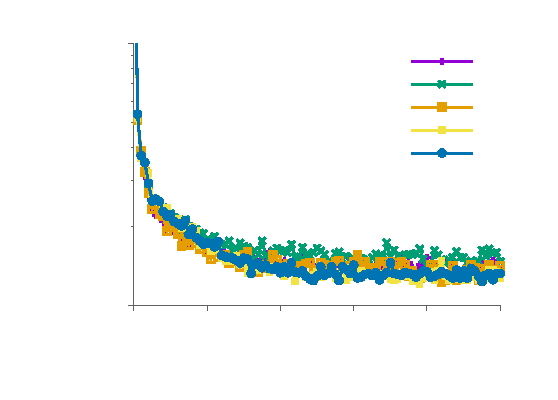
\includegraphics{chapter3/functionofepoch}}%
    \gplfronttext
  \end{picture}%
\endgroup

  \end{center}
  \caption{Evolution of the test error rate when learning MNIST using the square of a grid graph and for various normalizations, as a function of the epoch of training. The legend reads: ``l2'' means $\ell_2$ normalization of weights is used (with weights $10^{-5}$), ``Pos'' means parameters in $S$ are forced to being positive, and ``Norm'' means that the $\ell_1$ norm of each vector in the third dimension of $S$ is forced to 1.}
  \label{functionofepoch}
\end{figure}

\subsubsection*{Experiments with covariance graphs on Scrambled MNIST}

 We use a thresholded covariance matrix obtained by using all the training examples. We choose the threshold so that the number of remaining edges corresponds to a certain density $p$ (5x5 convolutions correspond approximately to a density of $p=3\%$). We also infer a graph based on the $k$ nearest neighbors of the inverse of the values of this covariance matrix ($k$-NN). The latter two are using no prior about the signal underlying structure. The pixels of the input images are shuffled and the same re-ordering of the pixels is used for every image. Dimension of the third rank of $S$ is chosen equal to $k$ and its weights are initialized random uniformly~\cite{glorot2010understanding}.
 The receptive graph layers are also compared with models obtained when replacing the first layer by a fully connected or convolutional one. Architecture used is the same as in the previous section. Results are reported on table~\ref{covar}.

\begin{table}[h]
  \caption{Error rates when topology is unknown on scrambled MNIST.}
  \begin{center}
    \bgroup
    \def\arraystretch{1.5}%  1 is the default, change whatever you need
    \begin{tabular}{|c|c|c|c|}
      \hline
      MLP & Conv5x5 & Thresholded ($p=3\%$) & $k$-NN ($k=25$)\\
      \hline
      1.44\% & 1.39\% & 1.06\% & 0.96\%\\
      \hline
    \end{tabular}
    \egroup
  \end{center}
  \label{covar}
  \end{table}

We observe that the receptive graph layers outperforms the CNN and the MLP on scrambled MNIST. This is remarkable because that suggests it has been able to exploit information about the underlying structure thanks to its graph.% The first version seems to have discovered a bit less information about the underlying structure. This might be explained by the fact that it has receptive fields of unequal sizes and might have required additional normalization.

\subsubsection*{Experiments with shallow architectures on Cifar10}

On Cifar10, we made experiments on shallow CNN architectures and replaced convolutions by receptive graphs. The first architecture used is the same than in the previous experiments on MNIST, and the second one is a variant of AlexNet~\cite{krizhevsky2012imagenet} using little distortion on the input that we borrowed from a tutorial of tensorflow~\cite{tensorflow2015-whitepaper}.
%On Cifar10, we use a variant of the AlexNet architecture applied on inputs with little distortion~\cite{krizhevsky2012imagenet}, borrowed from a tutorial of tensorflow~\cite{tensorflow2015-whitepaper}.
The latter is composed of two 5x5 convolutional layers of 64 feature maps, with max pooling and local response normalization, followed by two fully connected layers of 384 and 192 neurons.
%We switched each convolutional layer with receptive graph layers, but kept the pooling ones.
We compare two different graph supports: the one obtained by using the underlying graph of a regular 5x5 convolution, and the support of the square of the grid graph. Optimization is done with stochastic gradient descent on 375 epochs where $S$ is freezed on the 125 last ones. Circulant one-hot-bit intialization is used. These are weak classifiers for Cifar10 but they are enough to analyse the usefulness of the proposed layer. Exploring deeper architectures is left for further work. Results are summarized in table~\ref{cifar}. ``Pos'' means parameters in $S$ are forced to being positive, ``Norm'' means that the $\ell_1$ norm of each vector in the third dimension of $S$ is forced to 1, ``Both'' means both constraints are applied, and ``None'' means none are used.

\begin{table}[h]
  \caption{Accuracies of shallow networks on CIFAR10.}
  \begin{center}
    \bgroup
    \def\arraystretch{1.5}%  1 is the default, change whatever you need
    \begin{tabular}{|c|c|c|c|c|c|c|}
      \hline
      Support & \# convs & Learning $S$ & None & Pos & Norm & Both\\
      \hline
      \hline
      Conv5x5 & 1 & No & / & / & / & 66.1\%\\
      %\hline
      %Grid$^2$ & 1 & No & / & / & / & 66.8\%\\
      \hline
      Grid$^2$ & 1 & Yes & 67.3\% & 66.8\% & 67.1\% & 67.0\%\\
      \hline
      Conv5x5 & 2 & No & / & / & / & 87.0\%\\
      \hline
      Conv5x5 & 2 & Yes & 87.3\% & 86.9\% & 86.9\% & 87.5\%\\
      \hline
      Grid$^2$ & 2 & Yes & 87.1\% & 87.3\% & 87.6\% & 87.5\%\\
      \hline
    \end{tabular}
    \egroup
  \end{center}
  \label{cifar}
\end{table}

The receptive graph layers are able to outperform the corresponding CNNs by a small amount in the tested configurations, opening the way for more complex architectures.\newpage
 %\input{chapter3/neighbourhoodpreserving}\newpage

%
% Chapter 4
%

% \chapter{Industrial applications}
% \todo{}
% \vfill\minitoc\newpage

%
% Conclusion
%

% \chapter*{Conclusion}
% \label{chp:ccl}
% \addcontentsline{toc}{chapter}{\nameref{chp:ccl}}
% \todo{}

%
% Bibliography
%

\printbibliography[heading=bibintoc]

%
% Bin
%

% \setcounter{chapter}{-1}
% \chapter{Trash bin and more drafts}
% ... that we may use in some section.
% \vfill\minitoc\newpage

% \textcolor{red}{TODO: Rework 1.1}

%\section{Disambiguations and definitions}

% This thesis manuscript is about deep learning on \emph{irregular domains}. So what does it mean exactly ?

%% start of <see below> comment

% The term \emph{deep learning}, as introduced in the previous chapter, refers to a family of learnable models based on deep neural networks. The inputs of these models are \emph{signals} of a specific type. Learning is made over a training dataset of such signals. Hence, the term \emph{domain} as in \emph{irregular domains} refers to the definition domain of these input signals.

%% Shoud be put later, must make disambiguation with "unstructured" as well

% In this section we recall the basic naming convention in~\ref{basic}, of some definitions in~\ref{regularity}, and categorize the models we will review by the tasks for what they are designed in~\ref{tasks}.

\section{Naming conventions}
\label{basic}

\subsection{Basic notions}

Let's recall the naming conventions of basic notions.

A \emph{function} $f: E \rightarrow F$ maps objects $x \in E$ to objects $y \in F$, as $y = f(x)$.\\
Its \emph{definition domain} $\cd_f = E$ is the set of objects onto which it is defined. We will often just use the term \emph{domain}.\\
%Objects of its domain $\cd_f$ are mapped to objects of its \emph{codomain} $\cd_f^c= F$.\\
We also say that $f$ is \emph{taking values} in its \emph{codomain} $F$.\\
The \emph{image per $f$} of the subset $U \subset E$, denoted $f(U)$, is $\{y \in F, \exists x \in E, y = f(x)\}$.\\
The \emph{image of $f$} is the image of its domain. We denote $\ci_f$.\\
% The \emph{fiber} of the object $y \in \ci_f$ is the object $x \in E$ such that $y = f(x)$.\\
% The \emph{inverse image per $f$} of the subset $V \subset F$, denoted $f^{-1}(V)$ is $\{x \in E, \exists y \in F, y = f(x)\}$.
A vector space $E$, which we will always assume to be finite-dimensional in our context, is defined as $\bbr^n$, and is equipped with pointwise addition and scalar multiplication.% TODO reword?

A \emph{signal} $s$ is a function taking values in a vector space. In other words, a signal can also be seen as a \emph{vector} with an \emph{underlying structure}, where the vector is composed from its image, and the underlying structure is defined by its \emph{domain}.\\

For example, images are signals defined on a set of pixels. Typically, an image~$s$ in RGB representation is a mapping from pixels~$p$ to a 3d vector space, as $s_p = (r,g,b)$.

\textcolor{red}{TODO?: figure}
% quadillage , arrow ->, quadrillage remplie en 3 images
\begin{figure}

\end{figure}

\subsection{Graphs and graph signals}

%
\textcolor{red}{TODO: more defs on grid graphs and other graphs}
% need to define covariance graph, nearest neighbour
% Need to define grid graphs, regular grids from geometry, etc ...
% A regular grid graph is a nearest neighbor graph of a regular geometric grid
%

A \emph{graph} $G = (V, E)$ is defined as a set of nodes $V$, and a set of edges $E \subseteq\binom{V}{2}$. The words \emph{node} and \emph{vertex} will be used equivalently, but we will rather use the first.

A \emph{graph signal}, or \emph{graph-structured signal} is a signal defined on the nodes of a graph, for which the underlying structure is the graph itself.
A \emph{node signal} is a signal defined on a node, in which case it is a \emph{node embedding} in a vector space.

Although this is rarely seen, a signal can also be defined on the edges of a graph, or on an edge. We then coin it respectively \emph{dual graph signal}, or \emph{edge signal} / \emph{edge embedding}.

\emph{Graph-structured data} can refer to any of these type of signals.

\subsection{Data and datasets}

% Adjacency matrix, laplacian, etc ...
A dataset of signals is said to be \emph{static} if all its signals share the same underlying structure, it is said to be \emph{non-static} otherwise.\\
For image datasets, being non-static would mean that the dataset contains images of different sizes or different scales. For graph signal datasets, it would mean thats the underlying graph structures of the signals are different.

The point in specifying that objects of a dataset of a machine learning task are signals is that we can hope to leverage their underlying structure.

\textcolor{red}{TODO: figure}

\section{Disambiguation of the subject}

This thesis is entitled \emph{Deep learning models for data without a regular structure}.
So either the data of interest in this manuscript do not have any structure, or either their structure is not regular.

\subsection{Irregularly structured data}

By structured data, we mean that there exists an underlying structure over which the data is defined. This kind of data are usually modelized as signals defined over a domain. These domains are then composed of objects that are related together by some sort of structural properties. For example, pixels of images can be seen as located on a grid with integer spatial coordinates (a 2d cartesian grid graph).

It then come in handy to define the notions of structure and regularity with the help of graph signals.

\begin{definition}{Structure}\\
  Let $s: D \rightarrow F$ be a signal defined over a finite domain.\\
  An \emph{underlying structure} of the signal $s$ is a graph $G$ that has the domain of $s$ for nodes.\\
  A dataset is said to be \emph{structured}, if its objects can be modelized as signals with an underlying structure.\\
  It is said to be \emph{static} if all its objects share the same underlying structure, and \emph{non-static} otherwise.
\end{definition}

In other words, we chose to define ``structured data'' as ``graph-structured data'' by some graph. Hence we need to specify for which graphs this structure would be said to be regular, and for which it would not.

\begin{definition}{Regularity}\\
An underlying structure is said to be \emph{regular}, if it is a regular grid graph.
It is said to be \emph{irregular} otherwise.\\
A dataset is said to be \emph{regularly structured}, if the underlying structures of its objects are regular.
It is said to be \emph{irregularly structured} otherwise.
\end{definition}


\textcolor{red}{TODO: examples}
%% example images , example time series, example graph signals, example manifolds

\subsection{Unstructured data}

Data can also be unstructured. If the data is not yet embedded into a finite dimensional vector space, then we will be interested in embedding techniques used in representation learning. In the other case, it is often possible to fall back to the case of irregularly structured data. For example, vectors can be seen as signals defined over the canonical basis of the vector space, and the vectors of this basis can be related together by their covariances through the dataset. It is typical to use the graph structure that has the canonical basis for nodes, with edges obtained by covariance thresholding.

\textcolor{red}{TODO: examples}
%% give examples of unstructured data, graphs, scramble image datasets, etc..

%%%%%%%%%%%%%%%%%%%%%%%%%%%%%%%%%%%%%%%%%%%%%%%%%%%%%%%%%% END %%%%%%%%%%%%%%%%%%%%%%%%%%%%%%%%%%%%%%%%%%%%%%%%

%
% DRAFTS
%
\textcolor{red}{What follows is a draft}


%\section{Theoretical results on regularity and convolutions}

% idea : regularity of a domain implies with poset
% prop: if a domain has a poset, define translations and convolutions
% proving the converse too

\section{Datasets}

\section{Tasks} %% probably too early
\label{tasks}



\section{Goals}

\section{Invariance}

In order to be observed, invariances must be defined relatively to an observation. Let's give a formal definition to support our discussion.

...

\section{Methods}
\label{methods}\newpage
% % could be renamed: why not dense layers ?


\section{Expressivity analysis of dense versus sparse connectivity}

Let consider a tensor input $x$ of a neural network layer $l$. Without loss of generality, we consider that $x$ is a matrix of shape $n \times p$. Its rows are supposed structured by a graph $G = <V, E>$, with $|V| = n$, its columns are its feature maps.

In what follows, we discuss the expressivity and efficiency of a dense layer with $x$ as input versus a layer that would leverage $G$. We start with the regular case and continue onto non-regular structures.

\subsection{Strong regular case}

In the strong regular case, $G$ is a lattice graph such that a convolution is defined naturally on it. For example, this is the case where rows of $x$ defines ticks of a time series, or flattened pixels of an image.

Let consider a convolutional layer $c = (g_c,h_c)$ with padding, defined by $q$ filters of width $k$. Define $y_c$ its output of shape $n \times q$.

We are interested in knowing if there exists a dense layer that can efficiently replicate $c$.

Its connectivity matrix $W_c$ is of shape $np x nq$. Obviously, the function $g_c$ can be replicated by a dummy dense layer $d = (g_c,h_d)$ through $W_c$. However, whereas $c$ has only $kpq$ weights, $d$ has $n^2pq$. If we consider the families of neural networks $\cc$, $\cd$ spaned by their weights $\theta_c$, $\theta_d$, then we realize the $\cc$ is less expressive, but in the same time it is more efficient at representing its functions.

Let's define the notion of partial expressivity with respect to a family of functions.

Let $\cf$ a family of functions, $\cl$ a family of layer functions, and $\epsilon$ the approximation coefficient. For $f \in \cf$, define $S_{\epsilon}(\cl,f) = \{l \in \cl, d(l,f) < \epsilon \}$ and $S_{\epsilon}(\cl,\cf) = \displaystyle \bigcup_{f \in \cf} S_{\epsilon}(\cl,f)$.

\todo{reword above}

By abusing and anticipating future correction of this manuscript, we consider that $\cc$ and $\cd$ are vector spaces. We are interesting in 1. proving that $S_{\epsilon}(\cc,\cf)$ and $S_{\epsilon}(\cd,\cf)$ are also vector spaces, and 2. analysing for which $\cf$, $\frac{dim(S_{\epsilon}(\cc,\cf))}{dim(S_{\epsilon}(\cd,\cf))}$ is maximized.

Obviously 1. is false, so 2. is ill-posed (this draft is to be reworded afterward). Instead of using $dim$, we should rather use $card$. However they are potentially infinite families so we should rather use a notion of volume, except if we discretize. So let's discretize.

By the way, `'modified`' 2. is trivially maximized for $\cf = \cc$ (and then the ratio equals $1$), so let's weaken $\cf$ and say it's any family with translation equivariance. We are then interested in proving that if $\cf$ is the family on translation equivariant function (on this domains that has to be specified when rewriting this section), then $\frac{card(S_{\epsilon}(\cc,\cf))}{card(S_{\epsilon}(\cd,\cf))}$ is close to $1$. Equivariant in our context means commuting with translations (we should rather use the latter expression btw).

The result might be obtained without discretizing as convolutions with padding commutes with translations. Let's guess that they are close to other commuters. In fact that is even it. Proof with Fourier analysis.

% Let's discretize. We assume that entries of $x$ takes their values into a finite set $M = \{m_1, m_2, \ldots, m_r\}$.


% To unburden the notation, we'll assume $p=q=1$ and reshape to matrix-vector operations. A function $f \in \cf$ is defined by the values assigned to dimensions of $x$. For each $i \in \{1, 2, \ldots, n\}$, we define the grid tensor $\ca^f_i$, such that
% \begin{gather*}
% \forall j \in \{1, 2, \ldots, n\}, \forall i_j \in \{1, 2, \ldots, r\} \\
% \ca^f_i[i_1,i_2,\ldots,i_n] = f(x)[i] \Leftrightarrow \forall s \in \{1, 2, \ldots, n\}, x[s] = m_{i_s}
% \end{gather*}


\subsection{Draft}

The only dense layer that replicate $g_c$ is obtained through the connectivity matrix $W_c$. $\cd$ is more expressive, however less efficient as we are looking for equivariant functions. It happens that equivariant functions are exactly convolutions with padding.


\newpage
% \section{Conv drafts}


\todo{point}

In particular, we have
\begin{align*}
\forall s \in \cs(\Gamma), \widetilde\varphi(s) & = \widetilde\varphi\left( \displaystyle \sum_{g \in \Gamma} s[g] \delta_g \right)\\
& = \displaystyle \sum_{g \in \Gamma} s[g] \widetilde\varphi\left(\delta_g \right)\\
& = \displaystyle \sum_{g \in \Gamma} s[g] \delta_{\varphi(g)}\\
& = \displaystyle \sum_{v \in V} s[\varphi^{-1}(v)] \delta_{v}\\
\widetilde\varphi(s) & = \displaystyle \sum_{v \in V} \widetilde\varphi(s)[v] \delta_v\\
\end{align*}

So $\widetilde\varphi(s)[v] = s[\varphi^{-1}(v)]$ and $\widetilde\varphi(s)[\varphi(g)] = s[g]$. Let's simplify the notations with $\widetilde\varphi(s) = t$ and $\varphi(g) = v$, \ie $t[v] = s[g]$ as expected. We then define the group convolution on $\cs(V)$ as
\begin{align*}
(t_1 \ast t_2)[v] & = (s_1 \ast s_2)[g]\\
& = \displaystyle \sum_{h \in \group} s_1[h] \h{2} s_2[h^{-1}g]\\
& = \displaystyle \sum_{u \in V} s_1[\varphi^{-1}(u)] \h{2} h_u(s_2)[\varphi^{-1}(v)]\\
& = \displaystyle \sum_{u \in V} t_1[u] \h{2} \widetilde\varphi(h_u(s_2))[v]\\
\end{align*}



\begin{gather}
(t_1 \ast t_2)[v] = \displaystyle \sum_{u \in V} t_1[u] \h{2} h_u(t_2)[v]\\
\end{gather}


\todo{stop sign}




Recall that
\begin{align*}
\delta_{g}[h] & = \begin{cases} 1 & \text{if } h = g \Leftrightarrow \varphi(h) = \varphi(g)\\ 0 & \text{otherwise} \end{cases}\\
              & = \delta_{\varphi(g)}[\varphi(h)]
\end{align*}

\begin{align*}
s & = \displaystyle \sum_{v \in V} s[v] \h{2} \delta_v
\end{align*}






\todo{lemme on existence of uncountable linearly independent irrational family ?}

\begin{proposition} The group convolution on $\cs(\Gamma)$ has a unique neutral element which is the dirac signal on the identity tranformation.
\end{proposition}
\begin{proof}
Denote $\delta$ a neutral element for the group convolution. Note as because of the commutativity the group convolution, a left neutral element is also a right neutral element. We have $$s[h] = (\delta \ast s)[h] = \displaystyle \sum_{g \in \Gamma} \delta[g] \h{2} s[g^{-1}h]$$ which is true for any real valued signal. By chosing a signal $\pi$ having linearly independant irrational entries (and using the axiom of choice in case G is not finite), we obtain that $$\delta[g] = \begin{cases} 1 \text{ if } g = \id\\ 0 \text{ otherwise}\end{cases} \ie \quad \delta = \delta_{\id}$$
Conversely, $(\delta_{\id} \ast s)[h] = 1 . s[{\id}^{-1}h] = s[h]$.
\end{proof}











In other therms, if there is an isomorphism between $\Gamma$ and $V$, the group structure pass to $V$ as well as the definition of the group convolution.






To alleviate this issue, let's introduce the neutral elements $\delta$ of the convolution, and the neutral element $\id \in \Phi^*(V)$.


With the help of $\delta$, we follow the same process as in the proof of \propref{prop:equi}, see \eqref{eq:conv}, to construct the class of group convolutional operators which defines exactly the class of linear transformations that are equivariant to a certain group.


% \begin{definition}\textbf{Group convolution}\\



% \end{definition}








On graphs, this could be used provided we defined meaningful translations beforehand (see \secref{}). Another possibilty would be to search for invariances with respect to graph equivariances and derive a convolution operator similarly than for translations. This approach, which uses group convolutions~\citep{weinstein1996groupoids}, has already been discussed on regular domain to extend CNNs to other invariances than translational ones~\citep{cohen2016group,hoogeboom2018hexaconv}, as well as on spherical domain with rotation equivariant CNNs~\citep{cohen2018spherical}. As stated from the previous remark, the big advantage of this approach is that there is no loss of expressivity. However on graphs, this would be more challenging as it's not likely there exists transformations with equivariances. However, let's suppose we found such a set of transformations on a graph, then for \propref{prop:equi} to hold (instead as for regular translations), we see in the proof that they need to be bijective \eqref{eq:bij} and vertex dependent \ref{eq:conv}.




\subsection{}



\begin{definition}\textbf{Grounded set of transformations}\\
A set of transformations over a graph $\gve$, \emph{grounded} on a vertex $v_0 \in V$, denoted $\cp_{v_0} \subset \Phi(V)$, is a set that is in one-to-one correspondence with $V$, such that $\forall v \in V, \exists! p_v \in \cp_{v_0}, p_v(v_0) = v$.
\end{definition}

We have $\cp_{v_0} = \order(G) \in \bbn \cup \{+\infty\}$. For notational convenience we drop the subscript $_{v_0}$ in what follows.

\begin{definition}\textbf{$\cp$-equivariant convolution operator}\\
Let $\gve$ a graph, not necessarily a grid. Let $\cp$ a grounded set of transformations. Then, the  $\cp$-equivariant convolution operator $f_w$ is defined as
\begin{gather*}
\forall s \in \cs(V), f_w(s) = s \ast_{\cp} w = \displaystyle \sum_v s[v] \h{2} p_v(w)
\end{gather*}
\end{definition}

\begin{claim}\textbf{Characterization of $\cp$-eq. convolution operator}\\
The class of linear graph signal transformations that are equivariant to a grounded set $\cp$ is exactly the class of $\cp$-equivariant convolutive operations.
\end{claim}

\begin{proof}
By construction of $\cp$-equivariant convolutions, the proof is similar to the one of \propref{prop:equi}.
\end{proof}


\newpage
% \section{Conv graph Draft}

\subsection{Construction on Cayley graphs}

Let's suppose that from a vertex set $V$, we have constructed a convolution of the form $*_{\III}$, with $\Gamma \overset{\varphi}{\equiv} V$. One particular underlying graph structure would be define as the digraph $\vgve$, with $E=\{ (u,v), \exists g \in \Gamma, g(u) = v \}$. However, such graph would just be the complete digraph. To keep the information about the group $\Gamma$ somehow in $E$, without obtaining a complete digraph, we need to at least consider a generating set $\cu$. Hence, it is enough to define the edge set as $E=\{ (u,v), \exists g \in \cu, g(u) = v \}$. Conversely, an edge set $E$ with these hypotheses would then naturally support a graph convolution. This leads us to study the particular class of Cayley graphs~\citep{cayley1878desiderata,wiki:cayley}.

We now consider the class of Cayley (di)graphs~\citep{cayley1878desiderata,wiki:cayley} because the $\varphi$-equivalence property \eqref{eq:P} naturally holds on them.
\todo{rewrite and obtain: On a Cayley graph, there is $\varphi$ such that the subgroupoid of transformation that are EC is $\varphi$-equivalent (proof on $\cu$ then extended)}

\begin{definition}\textbf{Cayley graph}\\
Let a group $\Gamma$ and one of its generating set $\cu$. The \emph{Cayley graph} generated by $\cu$, is the digraph $\vgve$ such that $\Gamma \overset{\varphi}{\equiv} V$ and $E$ is such that:
\begin{gather*}
a \sim b \Leftrightarrow \exists u \in \varphi(\cu) \subset V, g_u(a) = b
\end{gather*}
\end{definition}

Cayley graphs allows to alleviate \ref{itm:d1} by summing onto the generating set~$\cu$ instead of onto~$\Gamma$.%, which also makes the convolution on Cayley graphs edge-constrained.

\begin{definition}\textbf{Cayley graph convolution}\\
\begin{align*}
\forall u \in V, (s_1 \ast_{\C} s_2) [u] & = \displaystyle \sum_{g \in \cu} s_1[g] \h{2} g(s_2)
\end{align*}
\end{definition}

Conversely, let a graph $\gve$ and a $\varphi$-equivalent subgroup $\Gamma \subseteq \Phi^{*}(V)$. Then we can generate a Cayley graphs with a generating set of $\Gamma$, and thus define a Cayley graph convolution. In particular, when transformations of~$\Gamma$ are edge-constrained, that would also be the case for this convolution on $G$, which leads us to study edge-constrained transformations.

\todo{operator and characterization}
\todo{which graph is a Cayley graph ?}

\subsection{Construction on graph groupoids}

% need abelian for path commutation. But can choose to take minimal path related to some choice. Cf bastnet.

\todo{work in progress}

On graphs, we notice that the property \eqref{eq:P} can be realized by transformations acting on edges. However, unless the graph is complete, these actions can't be composed everywhere to form another edge constrained action. The algebraic structure that posesses the same kind of properties than a group except that its composition law is not defined everywhere is called a groupoid. The following definitions clarify our discussion.

\begin{definition}\textbf{Groupoid}\\
A groupoid is a set equiped with a closed partial composition law, a unique identity element, and every unique inverses.
\end{definition}

\begin{remark}We use the convention than left and right inverses must be the same.
\end{remark}

\begin{definition}\textbf{Graph groupoid}\\
The \emph{groupoid} $\cp(G)$ of a graph $\gve$ is the set of its paths equiped with:
\begin{enumerate}
\item two maps $\psi$ and $\varphi$ that respectively map a path to its first and last element,
\item a closed partial composition law $gh$ defined if and only if $\psi(g) = \varphi(h)$, which concatenates $g$ behind $h$ and \sout{removes adjacent duplicate vertices} \textcolor{red}{to rewrite},
\item an inverse operator $\h{0}^{-1}$ which maps a path to its reverse,
\item an identity element $\id$ which is the path of length $0$.
\end{enumerate}
\end{definition}

\begin{remark}Recall from \defref{def:path} that a path can't contain adjacent duplicates.
\end{remark}

\begin{remark}Note that even though the composite path $gh$ has elements of $h$ before those of $g$ we write $gh$ instead of $hg$ because we'll need the left operand to act on the right one through functional notation $g(h)$.
\end{remark}

\begin{definition}\textbf{Graph $k$-groupoid}\\
The \emph{$k$-groupoid} $\cp_k(G)$ of a graph $\gve$, for $k \in \bbn^*$, is the groupoid obtained by restricting $\cp(G)$ to paths of length at most $k$ (the definition domain of its composition law is also further restricted by the length of the resulting paths in $\cp(G)$).
\end{definition}

\begin{definition}\textbf{$k$-Groupoid convolution}\\
Let a graph $\gve$. Let a subgroupoid $\Gamma \subseteq \cp_k(G)$. The $k$-groupoid convolution between two signals $s_1$ and $s_2 \in \cs(\Gamma)$ is defined as:
\begin{align*}
\forall h \in \Gamma, (s_1 \ast s_2) [h] & = \displaystyle \sum_{\substack{(a,b) \in \Gamma^2 \\ \st ab=h }} s_1[a] \h{2} s_2[b] \\
& = \displaystyle \sum_{\substack{g \in \Gamma\\ \st \varphi(g) = \varphi(h)}} s_1[g] \h{2} s_2[g^{-1}h]\\
& = \displaystyle \sum_{\substack{g \in \Gamma\\ \st \psi(g) = \psi(h)}} s_1[hg^{-1}] \h{2} s_2[g]
\end{align*}
\label{def:pconv}
\end{definition}

\begin{claim}\textbf{Path transformation}\\
Let a graph $\gve$. By identifying vertices with paths of length $1$, a path $g \in \cp(G)$ can act as a transformation on $v \in V$ through the composition law of $\cp(G)$. Also note that $g(v) = g(v^{-1})$.
\end{claim}

We can nom define the $k$-Groupoid convolution operator on $\cs(G)$ by restriction of the second operand from $\cs(\Gamma)$ to paths of length $1$:

\begin{definition}\textbf{$k$-Groupoid convolution operator}\\
Let a graph $\gve$. Let a subgroupoid $\Gamma \subseteq \cp_k(G)$. The $k$-groupoid convolution operator $f_w$ with parameter $w \in \cs(\Gamma)$ is defined as:
\begin{gather*}
\forall s \in \cs(\Gamma), \forall h \in \Gamma, f_w(s)[h] = (s \ast w)[h]
\end{gather*}
And when restricted to $\cs(G)$ it is defined as:
\begin{gather*}
\forall s \in \cs(G), \forall v \in V, f_w(s)[v] = \displaystyle \sum_{\substack{g \in \Gamma\\ \st \psi(g) = v}} s[g(v)] \h{2} w[g]\\
\forall s \in \cs(G), \forall v \in V, f_w(s)[v] = \displaystyle \sum_{\substack{g \in \Gamma\\ \st \varphi(g) = v}} s[g] \h{2} w[g^{-1}(v)]
\end{gather*}
\end{definition}

\begin{proposition}\textbf{Groupoid equivariance to $\Gamma$}\\
$k$-Groupoid convolution operators on $\cs(G)$ are groupoid equivariant to $\Gamma$ \ie
\begin{gather*}
\exists w \in \cs(\Gamma), f = w \ast . \Rightarrow
\forall v \in V, \forall g \in \Gamma \st \psi(g^{-1}) = v,
f \circ g [v]= g \circ f [v]
\end{gather*}
\end{proposition}

\begin{gather}
g(h(v)) maybe false
\end{gather}


Mini patron of todo:
\begin{itemize}
\item Equivariance to $\Gamma$ holds, proof
\item Converse of characterization does not hold yet, except on orbits
\item property for it to hold
\item relaxing one-to-one correspondence constraint but keeping other properties
\item other avenue instead of property: should make use of edges to build a group structure
\item ideal graph (lattice-regular)
\item if group is too much then just groupoid structure from edges is enough
\end{itemize}

\todo{finish this section}

\subsection{To rename}

% \begin{definition}\textbf{Infinite graph}\\
% An \emph{infinite graph} is defined by natural extension of the notion of graph $G=\langle V,E \rangle$ where $V$ and $E$ can be infinite. We denote $\order{G} = \infty$.
% \end{definition}

\begin{definition}\textbf{Graph automorphisms}\\
A graph automorphism of a graph $\gve$ is a bijection in the vertex domain $\phi: V \rightarrow V$ such that $\{u,v\} \in E \Leftrightarrow \{\phi(u), \phi(v)\} \in E$. We denote $\ca(G)$ the group of automorphism on $G$.

We denote by $\ce(\phi)$ the set of input-output mapping of $\phi$, defined as $\ce(\phi) = \{ (x,y) \in V^2, \phi(x) = y \}$.

A graph automorphism $\phi$ is said to be \emph{edge-constrained} (EC) if $\ce(\phi) \subseteq E$. We denote $\ca_{\EC}(G)$ the set of edge-constrained automorphism on $G$.
\end{definition}

\begin{definition}\textbf{Orthogonality}\\
Two graph automorphisms $\phi_1$ and $\phi_2$ are said to be orthogonal, if and only if $\ce(\phi_1) \cap \ce(\phi_2) = \emptyset$, denoted $\phi_1 \bot \phi_2$. They are said to be aligned otherwise.

Similarly, we define orthogonality of $r$ automophisms as $\phi_1 \bot \cdots \bot \phi_r \Leftrightarrow \ce(\phi_1) \cap \cdots \cap \ce(\phi_r) = \emptyset$
\end{definition}


\subsection{Lattice-regular graph}

\begin{definition}\textbf{Lattice-regular graph}\\
A lattice-regular graph is a regular graph that admits $r$ orthogonal edge-constrained automorphisms, where $r$ is its degree.
\end{definition}


%\subsubsection{Grids}{}

%\subsubsection{Lattices}

%\subsubsection{Spatial graphs}

%\subsubsection{Projections of spatial graphs}\newpage

%
% Post body
%

% % Temptative previsional plan
% \setcounter{chapter}{-1}
% \fakechapter{Temptative previsional plans}
% 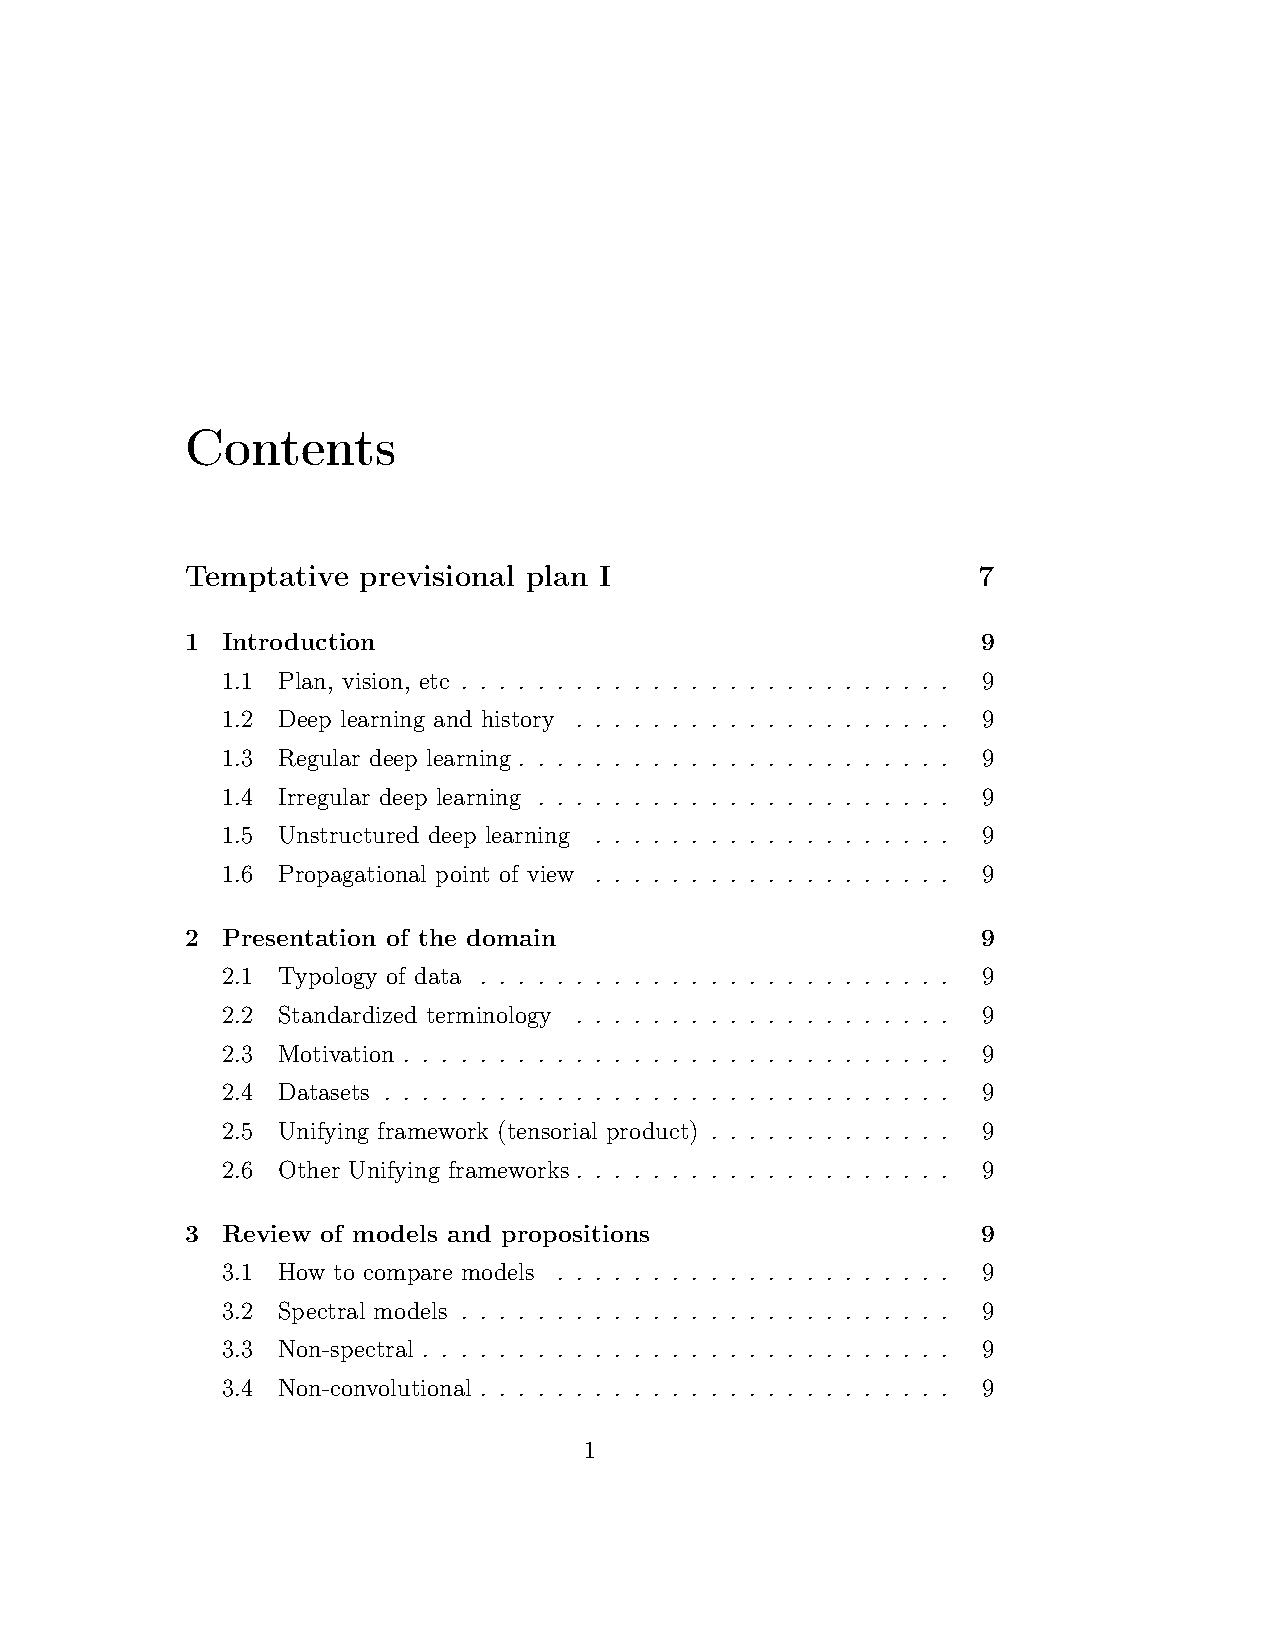
\includepdf[pages=1-7]{others/temptative_plan.pdf}

% % keywords and temptative titles
% \setcounter{chapter}{-1}
% \chapter{Keywords and temptative titles}
% \begin{keywords}
Deep learning,
representation learning,
propagation learning,
visualization,
structured,
unstructured regular,
irregular,
covariant,
invariant,
equivariant,
tensor,
scheme,
weight sharing,
graphs,
manifold,
euclidean,
signal processing,
graph signal processing,
time series,
time series database,
distributed application,
spatial-time series,
geo time series,
industrial applications,
warp 10,
warpscript,
...
\end{keywords} % to be put somewhere else
% \section*{Temptative titles}

\begin{itemize}
\item Learning propagational representations of irregular and unstructured data
\item Learning representations of unstructured or irregularly structured datasets
\item Propagational learning of unstructured or irregularly structured datasets
\item Learning tensorial representation of irregular and unstructured data
\item Tensorial representation of propagation in deep learning for irregular and unstructured dataset
\item Structural representation learning for irregular or unstructured data
\item Word for both ``irregularly structured'' + ``unstructured'' = ? (maybe ``unorthodox'' ?)
\item Unorthdox deep learning
\item ...
\item Deep learning of unstructured or irregularly structured datasets
\item Deep learning models for data without a regular structure
\item On structures in deep learning
\item On deep learning for when data is lacking a regular structure
\item Deep learning for non regularly structured data
\end{itemize}


\end{document}